% Options for packages loaded elsewhere
\PassOptionsToPackage{unicode}{hyperref}
\PassOptionsToPackage{hyphens}{url}
%
\documentclass[
  letterpaper,
]{book}
\usepackage{amsmath,amssymb}
\usepackage{lmodern}
\usepackage{iftex}
\ifPDFTeX
  \usepackage[T1]{fontenc}
  \usepackage[utf8]{inputenc}
  \usepackage{textcomp} % provide euro and other symbols
\else % if luatex or xetex
  \usepackage{unicode-math}
  \defaultfontfeatures{Scale=MatchLowercase}
  \defaultfontfeatures[\rmfamily]{Ligatures=TeX,Scale=1}
\fi
% Use upquote if available, for straight quotes in verbatim environments
\IfFileExists{upquote.sty}{\usepackage{upquote}}{}
\IfFileExists{microtype.sty}{% use microtype if available
  \usepackage[]{microtype}
  \UseMicrotypeSet[protrusion]{basicmath} % disable protrusion for tt fonts
}{}
\makeatletter
\@ifundefined{KOMAClassName}{% if non-KOMA class
  \IfFileExists{parskip.sty}{%
    \usepackage{parskip}
  }{% else
    \setlength{\parindent}{0pt}
    \setlength{\parskip}{6pt plus 2pt minus 1pt}}
}{% if KOMA class
  \KOMAoptions{parskip=half}}
\makeatother
\usepackage{xcolor}
\usepackage{longtable,booktabs,array}
\usepackage{calc} % for calculating minipage widths
% Correct order of tables after \paragraph or \subparagraph
\usepackage{etoolbox}
\makeatletter
\patchcmd\longtable{\par}{\if@noskipsec\mbox{}\fi\par}{}{}
\makeatother
% Allow footnotes in longtable head/foot
\IfFileExists{footnotehyper.sty}{\usepackage{footnotehyper}}{\usepackage{footnote}}
\makesavenoteenv{longtable}
\usepackage{graphicx}
\makeatletter
\def\maxwidth{\ifdim\Gin@nat@width>\linewidth\linewidth\else\Gin@nat@width\fi}
\def\maxheight{\ifdim\Gin@nat@height>\textheight\textheight\else\Gin@nat@height\fi}
\makeatother
% Scale images if necessary, so that they will not overflow the page
% margins by default, and it is still possible to overwrite the defaults
% using explicit options in \includegraphics[width, height, ...]{}
\setkeys{Gin}{width=\maxwidth,height=\maxheight,keepaspectratio}
% Set default figure placement to htbp
\makeatletter
\def\fps@figure{htbp}
\makeatother
\setlength{\emergencystretch}{3em} % prevent overfull lines
\providecommand{\tightlist}{%
  \setlength{\itemsep}{0pt}\setlength{\parskip}{0pt}}
\setcounter{secnumdepth}{5}
\newlength{\cslhangindent}
\setlength{\cslhangindent}{1.5em}
\newlength{\csllabelwidth}
\setlength{\csllabelwidth}{3em}
\newlength{\cslentryspacingunit} % times entry-spacing
\setlength{\cslentryspacingunit}{\parskip}
\newenvironment{CSLReferences}[2] % #1 hanging-ident, #2 entry spacing
 {% don't indent paragraphs
  \setlength{\parindent}{0pt}
  % turn on hanging indent if param 1 is 1
  \ifodd #1
  \let\oldpar\par
  \def\par{\hangindent=\cslhangindent\oldpar}
  \fi
  % set entry spacing
  \setlength{\parskip}{#2\cslentryspacingunit}
 }%
 {}
\usepackage{calc}
\newcommand{\CSLBlock}[1]{#1\hfill\break}
\newcommand{\CSLLeftMargin}[1]{\parbox[t]{\csllabelwidth}{#1}}
\newcommand{\CSLRightInline}[1]{\parbox[t]{\linewidth - \csllabelwidth}{#1}\break}
\newcommand{\CSLIndent}[1]{\hspace{\cslhangindent}#1}
\usepackage{booktabs}
\usepackage{amsthm}
\makeatletter
\def\thm@space@setup{%
  \thm@preskip=8pt plus 2pt minus 4pt
  \thm@postskip=\thm@preskip
}
\makeatother

%% Chapter formatting

%Options: Sonny, Lenny, Glenn, Conny, Rejne, Bjarne, Bjornstrup
%\usepackage[Lenny]{fncychap}

\usepackage{titlesec, blindtext, color} % titlesec needs `pandoc --variable subparagraph` to work
\definecolor{gray75}{gray}{0.75}
\newcommand{\hsp}{\hspace{20pt}}
\titleformat{\chapter}[hang]{\Huge\bfseries}{\thechapter\hsp\textcolor{gray75}{|}\hsp}{0pt}{\Huge\bfseries}
\makeatletter
\@ifpackageloaded{tcolorbox}{}{\usepackage[skins,breakable]{tcolorbox}}
\@ifpackageloaded{fontawesome5}{}{\usepackage{fontawesome5}}
\definecolor{quarto-callout-color}{HTML}{909090}
\definecolor{quarto-callout-note-color}{HTML}{0758E5}
\definecolor{quarto-callout-important-color}{HTML}{CC1914}
\definecolor{quarto-callout-warning-color}{HTML}{EB9113}
\definecolor{quarto-callout-tip-color}{HTML}{00A047}
\definecolor{quarto-callout-caution-color}{HTML}{FC5300}
\definecolor{quarto-callout-color-frame}{HTML}{acacac}
\definecolor{quarto-callout-note-color-frame}{HTML}{4582ec}
\definecolor{quarto-callout-important-color-frame}{HTML}{d9534f}
\definecolor{quarto-callout-warning-color-frame}{HTML}{f0ad4e}
\definecolor{quarto-callout-tip-color-frame}{HTML}{02b875}
\definecolor{quarto-callout-caution-color-frame}{HTML}{fd7e14}
\makeatother
\makeatletter
\makeatother
\makeatletter
\@ifpackageloaded{bookmark}{}{\usepackage{bookmark}}
\makeatother
\makeatletter
\@ifpackageloaded{caption}{}{\usepackage{caption}}
\AtBeginDocument{%
\ifdefined\contentsname
  \renewcommand*\contentsname{Table of contents}
\else
  \newcommand\contentsname{Table of contents}
\fi
\ifdefined\listfigurename
  \renewcommand*\listfigurename{List of Figures}
\else
  \newcommand\listfigurename{List of Figures}
\fi
\ifdefined\listtablename
  \renewcommand*\listtablename{List of Tables}
\else
  \newcommand\listtablename{List of Tables}
\fi
\ifdefined\figurename
  \renewcommand*\figurename{Figure}
\else
  \newcommand\figurename{Figure}
\fi
\ifdefined\tablename
  \renewcommand*\tablename{Table}
\else
  \newcommand\tablename{Table}
\fi
}
\@ifpackageloaded{float}{}{\usepackage{float}}
\floatstyle{ruled}
\@ifundefined{c@chapter}{\newfloat{codelisting}{h}{lop}}{\newfloat{codelisting}{h}{lop}[chapter]}
\floatname{codelisting}{Listing}
\newcommand*\listoflistings{\listof{codelisting}{List of Listings}}
\makeatother
\makeatletter
\@ifpackageloaded{caption}{}{\usepackage{caption}}
\@ifpackageloaded{subcaption}{}{\usepackage{subcaption}}
\makeatother
\makeatletter
\@ifpackageloaded{tcolorbox}{}{\usepackage[skins,breakable]{tcolorbox}}
\makeatother
\makeatletter
\@ifundefined{shadecolor}{\definecolor{shadecolor}{rgb}{.97, .97, .97}}
\makeatother
\makeatletter
\makeatother
\makeatletter
\makeatother
\ifLuaTeX
  \usepackage{selnolig}  % disable illegal ligatures
\fi
\IfFileExists{bookmark.sty}{\usepackage{bookmark}}{\usepackage{hyperref}}
\IfFileExists{xurl.sty}{\usepackage{xurl}}{} % add URL line breaks if available
\urlstyle{same} % disable monospaced font for URLs
\hypersetup{
  pdftitle={Putting Dental Calculus Under the Microscope},
  pdfauthor={Bjørn Peare Bartholdy},
  hidelinks,
  pdfcreator={LaTeX via pandoc}}

\title{Putting Dental Calculus Under the Microscope}
\author{Bjørn Peare Bartholdy}
\date{}

\begin{document}

%% Mandatory proefschrift page for Leiden PhD dissertations %%
\clearpage
\thispagestyle{empty}
\begin{center}
\Huge\textbf{Putting Dental Calculus Under the Microscope}\par
\vspace{\baselineskip}
\huge\textit{}\par
\vfill % this space will be whatever is left on the page
    \Large{Proefschrift}\par
    \vspace{\baselineskip}
    \linespread{1.3}
    \large{ter verkrijging van \\
    de graad van Doctor aan de Universiteit Leiden, \\
    op gezag van Rector Magnificus Dr.~H.J. Farnsworth, \\
    volgens besluit van het College voor Promoties \\
    te verdedigen op Wednesday 21 March 3020 \\
    klokke  uur \\[1.5cm]
    door} \\[1.5cm]
    \Large{Bjørn Peare Bartholdy}\par
    \vspace{\baselineskip}
    \large{geboren te Earth \\
    in the 20th century}
\end{center}
%% End: Proefschrift %%

%% Promotor and committee page %%
\clearpage
\thispagestyle{empty}

\noindent\begin{tabular}{p{8em} l}
    \large
    \textbf{Promotor}  & \large Dr.~Amanda G. Henry  \\ 
    \rule{0pt}{4ex}\large\textbf{Co-Promotor}  & \large Dr.~Annelou van
Gijn  \\ 
    \large
    \rule{0pt}{8ex}\textbf{Committee}  & \rule{0pt}{4ex}\large Dr.~Bernadette
Rostenkowski-Wolowitz  \\
    & \indent\textit{ZanGen
Pharmaceuticals} \\  & \rule{0pt}{4ex}\large Dr.~Amy Farrah Fowler  \\
    & \indent\textit{California Institute of
Technology} \\  & \rule{0pt}{4ex}\large Dr.~Sheldon Cooper  \\
    & \indent\textit{California Institute of
Technology} \\  & \rule{0pt}{4ex}\large Dr.~Leonard Hofstadter  \\
    & \indent\textit{California Institute of Technology} \\ 
\end{tabular}

\begingroup
\hspace{0.000001cm}
\vfill
\begin{flushleft}
\line(1,0){225} \\ %%%% Change colour of line to match chapters %%%%
\textbf{Front cover image:}  \\[0.5cm]
\textbf{Funding:} true 
\end{flushleft}
\endgroup
%% End: promotor and committee page %%

\frontmatter
\maketitle

\ifdefined\Shaded\renewenvironment{Shaded}{\begin{tcolorbox}[frame hidden, breakable, boxrule=0pt, enhanced, borderline west={3pt}{0pt}{shadecolor}, sharp corners, interior hidden]}{\end{tcolorbox}}\fi

\renewcommand*\contentsname{Table of contents}
{
\setcounter{tocdepth}{2}
\tableofcontents
}
\listoffigures
\listoftables
\mainmatter
\bookmarksetup{startatroot}

\hypertarget{hello}{%
\chapter*{Hello}\label{hello}}
\addcontentsline{toc}{chapter}{Hello}

\markboth{Hello}{Hello}

\frontmatter

\bookmarksetup{startatroot}

\hypertarget{acknowledgements}{%
\chapter*{Acknowledgements}\label{acknowledgements}}
\addcontentsline{toc}{chapter}{Acknowledgements}

\markboth{Acknowledgements}{Acknowledgements}

Where to begin? So many people helped shape this thesis, and are
therefore also to blame for this work.

\bookmarksetup{startatroot}

\hypertarget{open-science-statement}{%
\chapter*{Open Science Statement}\label{open-science-statement}}
\addcontentsline{toc}{chapter}{Open Science Statement}

\markboth{Open Science Statement}{Open Science Statement}

All materials and data, including the dissertation itself, are made
available to the best of my ability. All articles in association with
the dissertation are/will be Open Access.

Protocols available: \url{https://protocols.io/workspaces/byoc}\\
Code available: \url{https://github.com/bbartholdy}\\
Data available: TBD

\clearpage
\thispagestyle{empty}
\vspace*{3cm}

\textit{En bar røv at trutte i} \vspace*{\fill}

\par
\vspace*{4cm}

\begin{itemize}
\tightlist
\item
  Jan Bartholdy
\end{itemize}

\mainmatter

\bookmarksetup{startatroot}

\hypertarget{chap-intro}{%
\chapter{Introduction}\label{chap-intro}}

Dental calculus is becoming a popular substance in research on the
behaviour and biology of people in the past. You may also know it as
tartar or mineralised plaque. In other languages the word is often
related to ``tooth stones''. In fact, calculus is itself latin for
`pebble'. This was orginially used as a term for mathematical
calculations using counting stones, and only later used to describe
calicifications in the human body
(\url{https://www.etymonline.com/word/calculus}). This can be the cause
of some confusion, as calculus is also a branch of mathematics. If you
see the the term `calculus' in this disseration, you can safely assume
that I'm referring to stuff that grows on your teeth and for which you
receive lectures from your dentist, and not the topic you dreaded in
high school.

I will briefly describe the formation of dental calculus here, but for a
more thorough review of the entire process I refer you to
\protect\hyperlink{chap-background}{chapter 2}. Dental calculus is
formed from dental plaque, a substance that forms on you teeth and
consists mainly of bacteria and a surrounding structure called the
extracellular matrix. When the local environment within and around the
plaque reaches a favourable alkaline pH, both the extracellular matrix
and bacteria within will calcify (Jin \& Yip, 2002; D. J. White, 1997).
The alkaline pH causes minerals (especially calcium and phosphate) from
saliva to enter the plaque, causing the extracellular matrix and
eventually also the bacteria to harden, resulting in a concrete-like
deposit on the surface of the teeth. The process repeats itself when new
bacteria colonise the surface of the newly formed dental calculus,
creating a layered structure, though somewhat disorganised (Akcalı \&
Lang, 2018; Jepsen et al., 2011). Dental plaque can accumulate more
easily on teeth (and dental calculus) because they are a hard,
non-shedding surface. Most of the surfaces in our mouth are covered by a
layer of cells called the oral epithelium. These cells are continuously
renewed as new cells are formed and dead cells fall off (Squier \&
Finkelstein, 1998). This constant turnover means that it is difficult
for bacteria to build the communities they require for producing
biofilms. Enamel, the white substance that covers the crown of your
teeth, behaves differently. It stops growing when the tooth has fully
formed. After that, there is no renewal. This allows bacteria to
continue to grow and develop communities if there is no intervention
from you (or your dentist). Dental plaque can trap a variety of
different microparticles, including bacteria, human proteins, and small
debris from the food we eat (De La Fuente et al., 2013; Hendy et al.,
2018; Henry \& Piperno, 2008). When the plaque mineralises, it can
preserve these microparticles over long periods of time, even after the
person whose teeth provided a home for the calculus has died.

Also, the main crystal forms in calculus strongly bind DNA, making
calculus a fantastic source of ancient DNA (aDNA) from the mouth
(Warinner et al., 2015). This is probably why archaeologists have become
increasingly interested in dental calculus.

\hypertarget{intro-arch}{%
\section{Dental calculus in archaeology}\label{intro-arch}}

The main archaeological interest in dental calculus is to explore
research questions involving diet and the evolution of the oral biome
and oral health (Adler et al., 2013; Fellows Yates et al., 2021; Henry
\& Piperno, 2008; Warinner, Rodrigues, et al., 2014; Warinner, Hendy, et
al., 2014). These topics have not changed much since the early uses of
dental calculus in archaeological research, but the methods certainly
have.

In the past, some researchers would consider calculus a nuissance
because it obscured tooth and root morphology (Scott, 2015); this had
made a lot of people very angry and been widely regarded as a bad move
(Adams, 2002c, p. 1). A simple three-stage archaeolgy-specific scoring
method was developed (Brothwell, 1981), similar to a common clinical
scoring sytem (J. G. Greene \& Vermillion, 1964), and is still widely
used today. More detailed methods are also available (Dobney \&
Brothwell, 1987; T. R. Greene et al., 2005).

\begin{figure}

{\centering 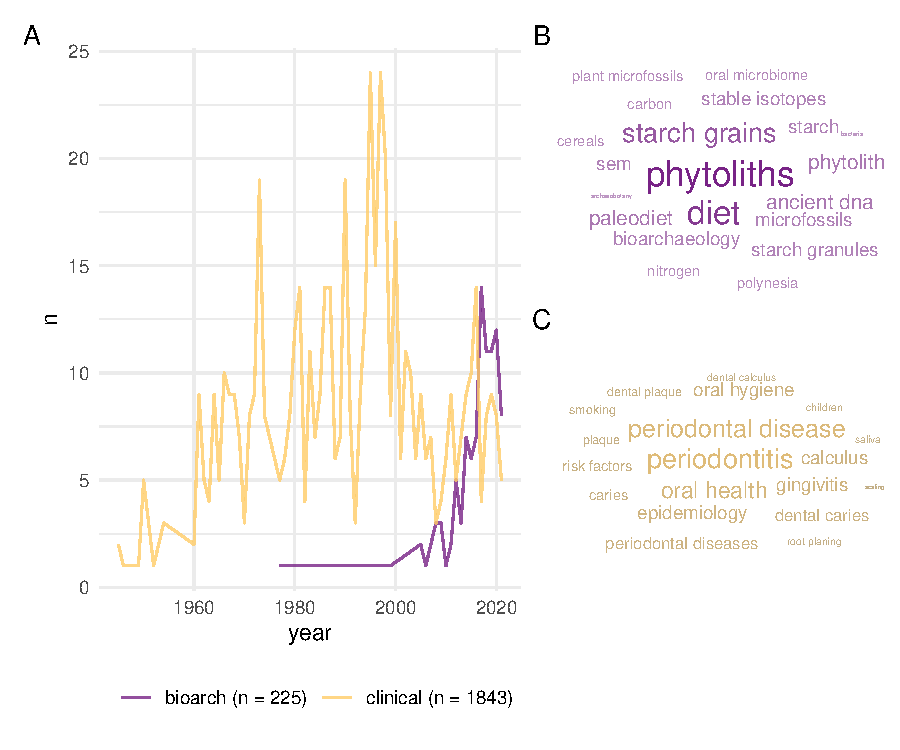
\includegraphics{01-intro_files/figure-pdf/fig-plot-and-wordclouds-1.pdf}

}

\caption{\label{fig-plot-and-wordclouds}Plot of articles with the term
`dental calculus' in the title.}

\end{figure}

Perhaps the most common uses of dental calculus is to try and recreate
the diet of past people and populations
(Figure~\ref{fig-plot-and-wordclouds}B). One of the ways to do this is
dissolving the calculus in a weak acid, a decalcifant, or mechanically
breaking it up. This process releases any fragments of plants that were
trapped within the calculus and can be identified, for example with a
microscope. The tricky part is not destroying the plant fragments when
releasing them from the calculus. As far as I can tell, the first
attempt at this was the extraction of phytoliths (silicified plant
remains) from the teeth of cows, sheep, and horses (Armitage, 1975).
This was a somewhat isolated use-case, and it didn't really catch on
until the 1990s (Ciochon et al., 1990; Middleton 1990, in W. D.
Middleton \& Rovner, 1994). The first extractions from human teeth
followed shortly (Fox et al., 1996), and there are now studies using
plant microremains (especially starch granules and phytoliths) from
dental calculus to infer diet in past peoples from across the world,
including Rapa Nui (Dudgeon \& Tromp, 2014), China (T. Chen et al.,
2021), Europe (Fiorin et al., 2021), and more (Buckley et al., 2014;
Henry \& Piperno, 2008; Mickleburgh \& Pagán-Jiménez, 2012). The durable
nature of dental calculus also means that microremains within it can
survive for millenea, allowing us to look at the diets of early humans
and other hominins (Buckley et al., 2014; T. Chen et al., 2021; Hardy et
al., 2009; Hardy et al., 2012; Henry et al., 2012, 2014; Henry \&
Piperno, 2008; Piperno \& Dillehay, 2008). It's also considered useful
because it represents a more recent and direct source of diet than teeth
or other bones, since the turnover is much quicker in calculus than
bone. Calculus can form within weeks at any point during an individual's
life and may indicate direct consumption, while bone can take years to
incorporate a dietary signal. Enamel stops forming after the last tooth
has developed, and the turnover of dentin is very limited (Hillson,
1996).

That bacteria can become trapped within calculus has been known to
archaeologists for a while (Brothwell, 1981, ; Vandermeersch et al.,
1994), but it wasn't utilised in archaeological research until DNA
extraction started to become more accessible (De La Fuente et al.,
2013). Dental calculus then became part of the third scientific
revolution in archaeology. The early studies focused on oral health in
the past (Adler et al., 2013; De La Fuente et al., 2013; Warinner,
Rodrigues, et al., 2014). Bacteria have shorter lifespans than humans
which makes them useful when studying the evolution of bacteria in the
human mouth (De La Fuente et al., 2013; Fellows Yates et al., 2021).
Diet has also been a focus of paleogenetic research. This has mainly
been addressed by considering how long-term changes in the patterns of
bacteria within the mouths of our ancestors have changed that could be
related to changes in diet. Just like we adapt to deal with various
diseases, climates, etc., we also adapt to changes in our diet (Adler et
al., 2013; Fellows Yates et al., 2021). Directly identifying genetic
markers of plants and animals within dental calulus is difficult, but
not impossible (see Warinner, Hendy, et al. (2014)). Most of the DNA
within dental calculus will be oral bacteria, and this will overwhelm
the signal from plant DNA. Plants are also really complicated because
the plant DNA only makes up a fraction of the DNA extracted from
calculus, which is overwhelmed by the presence of endogenous and
bacterial DNA (personal communication with Zandra Fagernäs, James
Fellows Yates, and Nikolay Oskolkov in the SPAAM community) (Fagernäs et
al., 2022). A newer field of biomolecular archaeology, paleoproteomics,
may be able to {[}resolve{]} this issue by targeting to plant proteins.
Hendy and coauthors were able to identify a number of these in dental
calculus, as well as proteins from cereals, and milk proteins from
different sources (Hendy et al., 2018).

To a lesser extent, the presence and amount of dental calculus on teeth
has been used as an indicator of dental health (Drewett, 1975; Lieverse
et al., 2007; Sagne \& Olsson, 1977; Zhang, 1982). Pilloud \& Fancher
(2019) explored the terms associated with a number publications on
dental or oral health, dental calculus came up as one of them; albeit
not the most common, which was (unsurprisingly) dental caries
(Figure~\ref{fig-dental-terms}). More recently Yaussy \& DeWitte (2019)
looked at how it relates to overall health in a population, not just
oral health. They suggest that individuals with more calculus are more
at risk than individuals with less or no calculus.

\begin{figure}

{\centering 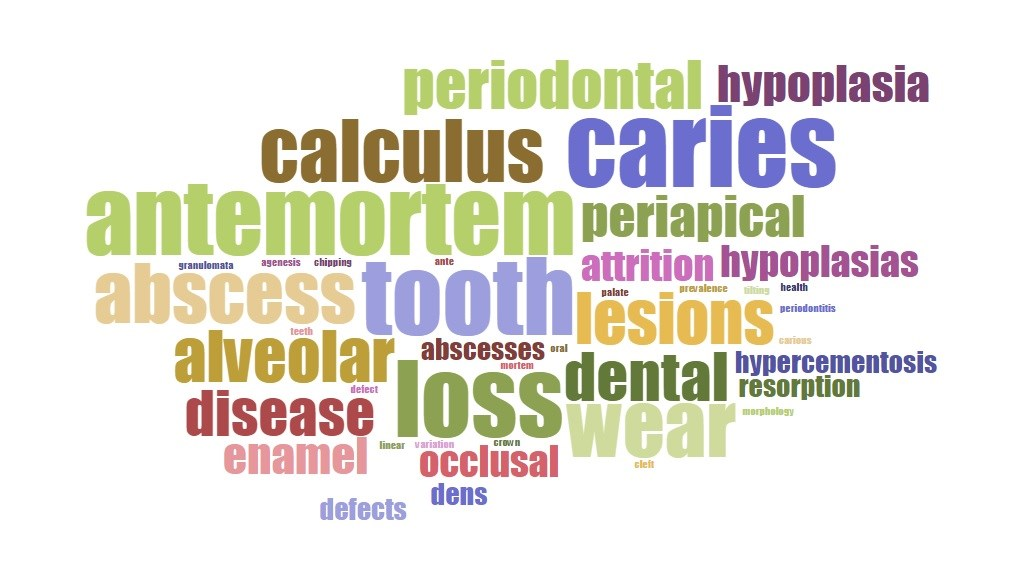
\includegraphics{figures/wordcloud.png}

}

\caption{\label{fig-dental-terms}Word cloud of most common dental terms
in articles. Figure is from Pilloud \& Fancher (2019), Figure 1}

\end{figure}

This wide range of applications, and the fact that it's pretty much
ubiquitous in the past (thanks to poor oral hygiene), makes it a really
exciting area for the future of archaeological research! That being
said, the study of dental calculus doesn't seem to fit into any
predefined areas of study within (and beyond) archaeology. Most
researchers seem to see it as a means to the information contained
within, rather than being worth studying in its own right (with some
exceptions, of course). This can be problematic. Other than what we can
see with our current methods, what do we really know about dental
calculus and how its growth and structure affect the reliability of
these methods and potentially distort our interpretations of the past?

\hypertarget{intro-what}{%
\section{What is dental calculus?}\label{intro-what}}

First, we must answer a single, surprisingly difficult question: What is
dental calculus? I'm not referring to its formation or composition,
which I briefly described \protect\hyperlink{intro}{above}. How do we
categorise it? Is it a dental disease? An oral health condition? A
byproduct of oral conditions? To answer this, it's necessary to look at
various definitions of oral health. Definitions in an introduction are a
little cliché and tedious, but often necessary. Definitions of oral
health are often purposefully (and confusingly) broad, because oral
health is a very complex topic. It extends beyond physical well-being
and into the realms of emotional and social comfort. The World Dental
Federation (FDI) defines oral health as the ability to perform mouth-
and face-related functions with confidence and without pain (including
smiling, speaking, eating, etc.) (\emph{{FDI}'s Definition of Oral
Health \textbar{} {FDI}}, n.d.)
(\url{https://www.fdiworlddental.org/fdis-definition-oral-health}). Both
the World Health Organisation (WHO) and FDI take a similar approach to
defining oral conditions, giving a list of conditions that cause
discomfort, pain, disfigurement, or death. The list includes the dental
conditions tooth decay (caries), gum disease (periodontal disease), and
dental trauma, but not dental calculus (\emph{Oral Health}, n.d.)
(\url{https://www.who.int/news-room/fact-sheets/detail/oral-health}).
While these are not likely to cause death, they are often the source of
physical and emotional discomfort, and may cause further health
complications if they are not dealt with in a timely fashion.

Dental calculus and dental plaque are not considered oral conditions
according to WHO. In fact, dental plaque is part of the normal
functioning of our oral biome (Philip D. Marsh, 2006). When plaque
reaches a certain level of acidity over a prolonged period of time, the
normal functioning of the bacteria within the plaque may shift towards a
disease-causing function. The biofilm will cause the surface of the
enamel to demineralise, eventually resulting in a cavity (or caries).
Dental caries are unequivocally considered a dental disease. If,
instead, the biofilm calcifies, dental calculus is the result. Its
status in oral health is questionable.

Dental calculus is not known to be painful, nor does it affect the
ability to perform the functions listed above. However, with continued
accumulation, it may affect the confidence of the person performing
these tasks (Collins \& Freeman, 2007), and in extreme cases it can
affect function (Balaji et al., 2019). Most of the virulence and
disease-causing potential is lost when the bacteria within dental plaque
calcify (Akcalı \& Lang, 2018). It has been shown to contain pockets of
living bacteria that can be detrimental to oral and dental health (B. T.
K. Tan, Gillam, et al., 2004; B. T. K. Tan, Mordan, et al., 2004). The
rough, porous surface of dental calculus is also a great place for
bacteria to attach more easily and develop a new layer of plaque on the
surface of the calculus. This is likely why there is often a correlation
(NOT causation) between dental calculus and periodontitis, especially
subgingival calculus (Jepsen et al., 2011; D. J. White, 1997). Since it
seems to fulfill some of the criteria of an oral condition, it should be
considered as such, at least under the definitions provided by WHO and
FDI. Is it also a dental disease? While it does grow on the surface of
teeth, it doesn't seem to affect the underlying enamel. And while there
is a relationship with periodontal disease (which has been defined as a
dental disease), the nature of this relationship is still under debate,
with calculus likely being a secondary contributor (Jepsen et al.,
2011). As such, we can probably limit the definition to an oral
condition and not necessarily a dental disease (Pilloud \& Fancher,
2019). In fact, dental calculus is quite hard, so a layer of dental
calculus on a tooth can actually protect it from wearing down (although
there are better options).

\hypertarget{intro-study}{%
\section{The study of dental calculus}\label{intro-study}}

It seems that the researchers who are studying dental calculus approach
it from a wide range of different fields and backgounds, including
genetics, proteomics, botany, and (bio)archaeology. The paleogeneticists
mine it for the wealth of information it contains on oral health and
disease in the past (Fellows Yates et al., 2021; Warinner, Rodrigues, et
al., 2014). Paleodiet researchers extract microremains and residues from
food (Henry \& Piperno, 2008; Mickleburgh \& Pagán-Jiménez, 2012) to
infer dietary practices. Paleopathologists use it to infer overall
health in a given population (Yaussy \& DeWitte, 2019). This leaves
research output from studies of calculus scattered across multiple
venues, with no clear gathering point. I think it's fair to say that
dental calculus should be included in discussions of pathological oral
conditions, even if its role is secondary. But who is currently studying
dental calculus as a substance in its own right? And why do we need to
learn more about it if we're just interested in what's inside? Related
discussions have started to take place in recent years (Bucchi et al.,
2019; Anita Radini \& Nikita, 2022; Wright et al., 2021).

The lack of a specific field of study for dental calculus to belong may
be related to how it's taught to students (and if it's taught at all).
Textbooks from the more established fields in bioarchaeology are
probably a good indicator of the teaching curricula, which also impacts
research focus. The most popular osteoarchaeology textbooks only briefly
mention dental calculus as more of a footnote than anything else. A
couple of lines describing what it is (usually `mineralised plaque') and
that it can contain food debris and bacteria T. D. White et al. (2011).
They're not wrong. Diseases that manifest themselves in the skeleton as
lesions on the bones have a very clear home in paleopathology. No one
questions whether or not the degeneration of vertebrae from tuberculosis
should be included in the paleopathology textbooks (at least not as far
as I'm aware).

These textbooks often include chapters on dental disease, where more
detailed descriptions of dental calculus are usually found (e.g. Roberts
\& Manchester, 2007; Waldron, 2020). Dental caries, calculus' more
famous sibling, will often get a few pages. In some cases, dental
calculus may even be hidden within a section on periodontal disease or
plaque (Aufderheide et al., 1998; e.g. Ortner, 2003). The focus of these
(sub)sections is varied, with some simply describing what it is, and
others giving brief discussion on the relationship between calculus and
periodontal disease. A more detailed section was dedicated to dental
calculus in \emph{Ortner's Identification of Pathological Conditions in
Human Skeletal Remains}, with a detailed description of formation,
structure, and application in (biomolecular) archaeology (Kinaston et
al., 2019). The description extends well beyond any (paleo)pathological
significance of dental calculus. Can we fault the authors/editors for
not giving it more attention? After all, it's not a dental disease, and
its relationship with other dental diseases is unclear. What is clear,
is that it has implications for oral health, and, for that very reason,
could be addressed more extensively in paleopathology; certainly in the
textbooks that include dental disease.

On the surface, dental anthropology seems like a more suitable home for
the study of dental calculus. However, it's not included in \emph{A
Companion to Dental Anthropology}, an otherwise great resource on
studying archaeological teeth. The editors briefly acknowledge the
valuable information gained from calculus and that it holds a lot of
potential; but that's it (Scott, 2015). Other notable absences include
textbooks such as \emph{Technique and Application in Dental
Anthropology} and \emph{New Direction in Dental Anthropology} (Townsend
et al., 2012), both of which dedicate considerable attention to dental
caries. Hillson's \emph{Dental Anthropology}, a book that I consider to
be the `bible' for dental anthropology, has a section on dental calculus
in the Dental Disease chapter. It covers a basic description, the
composition, microscopic structure, methods used for recording
archaeological calculus, and the distribution in the dentition
(i.e.~which teeth are more prone to calculus buildup) (Hillson, 1996).

Considering these are entire books devoted to the dentition, is it odd
that there is often only a few paragraphs (if that) on dental calculus?
After all, dental calculus isn't even a dental disease. The only
function teeth serve in the growth of dental calculus is as a suitable
surface on which to attach. Continued development and growth of dental
calculus relies on the conditions inside the mouth. It is of course an
important role, as dental calculus is seemingly unable to form on other
surfaces in the oral cavity. Sorry to do this to you again, but we need
more definitions. The \emph{Medical Dictionary for the Dental
Professions (2012)} defines dental anthropology as:

``a branch of physical anthropology concerned with the origin,
evolution, and development of dentition of primates, especially humans,
and to the relationship between primates' dentition and their physical
and social relationships.'' (in Irish \& Scott, 2015).

It could certainly be considered part of the development of dentition in
primates (if you consider both `development' and `dentition' more
broadly). Perhaps the description on the Dental Anthropology
Association's (DAA) website gives more room for interpretation:

``Dental anthropology utilizes the dentitions of humans and other
non-human primates--both past and present--to answer questions of
anthropological interest. These questions can include (but are by no
means limited to): How are individuals and populations related? What did
their diet look like? How healthy were they?'' (\emph{Dental
{Anthropology Association}}, n.d.)
(\url{http://www.dentalanthropology.org/}, accessed 30-Nov-2021).

This description more directly addresses a dietary and health
perspective, which certainly applies to dental calculus, as long as you
consider it part of the dentition. It's possible we'll see dental
calculus included in more detail in future textbooks, given how it has
increased in popularity over the last decade or so.

Since the use of dental calculus in biomolecular archaeology is
relatively new, there are fewer available textbooks, and it rarely has a
dedicated course. The most common place to find descriptions of dental
calculus is, therefore, journal articles. There will be a short
paragraph on dental calculus formation (and sometimes composition) in
the introduction section. These are quite variable and are often limited
by the word count of the journal. Despite this, the descriptions will
often be as long, if not longer, than the sections in textbooks devoted
to dental calculus (Velsko et al., 2019). The focus of these paragraphs
are generally the same. They describe the formation and mineral
composition of dental calculus, and provide some examples of how dental
calculus has been used in related studies (not unlike the beginning of
this chapter).

\hypertarget{what-do-we-know}{%
\section{What do we know?}\label{what-do-we-know}}

What we know about dental calculus and the influence of diet was
reviewed in an article aimed at (bio)archaeologists. The overall
conclusion reached in the article: it's still pretty unclear (Lieverse,
1999). High-protein diets are linked to an increase of urea, which is
linked to an increase in oral pH, which is linked to mineral deposition
(Dibdin \& Dawes, 1998; Wong et al., 2002). BUT, protein may also
inhibit crystalisation (S. Hidaka \& Oishi, 2007). Starch consumption
has been linked to increased rates of caries in early farming
populations. This is consistent with \emph{in vitro} testing, at least
for starches high in amylose content. So a high-starch diet causes
caries, not calculus, right? Well, starches with a high amylopectin
content are linked to increased calcification (S. Hidaka \& Oishi,
2007). It likely depends on what is consumed along with the starch
(Saburo Hidaka et al., 2008). There is also some (\emph{in vitro})
evidence to suggest that silica may promote dental calculus formation by
promoting mineral precipitation, i.e.~the transfer of minerals from
saliva to the biofilm (Damen \& Ten Cate, 1989).

Another aspect of diet and dental calculus where we are still looking
for answers, is the process that causes fragments of food and other
environmental materials to become entrapped in the dental calculus. We
know that it happens. Decades of research has shown dental calculus to
be a seemingly unlimited resource for dietary substances. We don't know
exactly how this happens, and herein lies the potential for bias.
Efforts have been made to understand how much of the consumed food makes
it into the calculus. These include studies on modern humans (Leonard et
al., 2015) and non-human primates (R. C. Power et al., 2015; Robert C.
Power et al., 2021), where food intake is meticulously documented, and
calculus subsequently analysed. These studies have common findings; the
amount of the diet that becomes trapped in the dental calculus of any
one person has no clear relationship to the amount of food that was
consumed. The most likely reason is that the formation of dental
calculus differs between people (R. C. Power et al., 2015). So, it's not
a great way to study the diet of a single person, but generally suitable
to study patterns in the diet of a population. The more people you
study, the more likely you are to gain a complete picture of the diet in
a population The fact that we can still see (in some cases, literally)
remains that were consumed thousands of years ago is pretty cool. We
just need a better understanding of why the record of diet from dental
calculus differs from the actual intake of food. This will allow us to
make more robust interpretations about past dietary practices. Something
that may influence the dietary record that we get from calculus is the
method we use to extract the dietary remains from calculus. Our
understanding of dental calculus extraction methods is improving, with
studies looking at the effect of various acids used to dissolve calculus
(commonly EDTA or HCl) (Bucchi et al., 2019; Soto et al., 2019; Tromp et
al., 2017); as is our understanding of how the choice of tooth may
affect our results (Fagernäs et al., 2021).

These studies provide valuable insights into potential biases of our
sampling methods and the representation of diet within dental calculus,
with a minor caveat. Most of these studies have been conducted on living
primates or archaeological remains. An issue with using living (or once
living) organisms is the inability to control factors related to the
variability between subjects. Basically, studying humans is messy and
complicated because we're all unique. It's a lovely sentiment but it can
make for some messy science. Not bad science (not at all!). Just messy.
A method of study that offers more control, is the growth of plaque and
calculus in a lab. This allows us to control many of the things that we
are difficult to control in humans, such as the bacteria that colonise
our mouth, where each person has a pretty unique makeup of bacteria. We
also have a very unique genome (with the exception of identical twins)
that plays a role in how quickly we form calculus in our mouth (if at
all). Certain enzymes start digesting our food before as soon as it
enters our mouth, and the activity of these enzymes fluctuates
throughout the day, causing a lot of variability both within and between
individuals. Finally, the number of microremains that enter our mouth
over days, weeks, months, can be very different between people, even
with the same diet. All these things can muddy the results of research
on living subjects, where a lab-grown approach can help tease out
confounding factors. I don't believe research conducted on lab-grown
biofilms can in any way replace studies with modern or archaeological
individuals, nor should they. But it can complement these studies by
zooming in on certain aspects that are too difficult to isolate in
(once-)living people.

Often we can draw from clinical studies as there are common goals,
e.g.~discovering the aetiology and/or presentation of a disease.
However, the motivation driving the studies in archaeology and dental
research are inherently different; although, there is certainly overlap
in some areas (Figure~\ref{fig-plot-and-wordclouds}B and C). There is
more interest in preventing dental calculus from forming in the first
place, so most studies focus on anti-microbial treatments and inhibition
of biofilm formation and plaque buildup (Exterkate et al., 2010).
Archaeologists are more interested in questions related to how diet
influences the growth of biofilms, and how fragments become embedded
inside, and what we can say about diet. Further, the interest in dental
calculus as a field of clinical research has been declining since the
2000s, which, as far as I'm aware, is when the last studies growing
dental calclulus in a lab were conducted. We can see this by the number
of clinical articles with the term dental calculus in the title
(Figure~\ref{fig-plot-and-wordclouds}A). And they certainly aren't
interested in how food debris becomes trapped inside our calculus.
Dental calculus has also become less of a problem with the use of modern
dental hygiene practices and regular visits to the dentist (Velsko et
al., 2019).

To summarise: Bioarchaeologists are interested in how dental calculus
relates to dental and general health; paleodietary researchers are
interested in the food remains that are trapped inside; paleogeneticists
are interested in accessing the oral bacteria that have been fossilised
within; clinial dentistry views it as a nuisance to be removed and,
ideally, prevented from forming in the first place. This lack of
systematic research specifically devoted to dental calculus as a
substance, rather than a means to an end, leaves a lot of questions
regarding the expected behaviour of dental calculus and how information
from the past becomes trapped inside. To summarise the summary: we need
to ask more basic questions about dental calculus.

\hypertarget{what-dont-we-know}{%
\section{What don't we know?}\label{what-dont-we-know}}

\hypertarget{intro-aims}{%
\section{Aims}\label{intro-aims}}

This disseration is a contribution to a dental-calculus-centric body of
knowledge, and addresses a gap in the fundamental research on dental
calculus to further our understanding of how we can use dental calculus
to reconstruct the diets of people in the past. The main focus is the
development, validation, and application of a calcifying oral biofilm
model to inform interpretations on archaeological dental calculus.

In short, can I grow calculus in the lab? Is what I'm growing actually a
substance that resembles calculus? And can the model be used to inform
archaeological research; specifically, how should we interpret the food
debris extracted from dental calculus?

\hypertarget{thesis-outline-and-structure}{%
\section{Thesis outline and
structure}\label{thesis-outline-and-structure}}

If you have made it to this point, you have probably read most of
\protect\hyperlink{chap-intro}{Chapter 1}, in which I provide some
context to the study of dental calculus in archaeology and identify some
areas that could benefit from further investigation.

\protect\hyperlink{chap-background}{Chapter 2} provides some background
information on oral biofilms and oral biofilm models in more detail than
I can do in the research articles included in Chapters 3 and 4. So if
you're already well-versed in oral microbiology, feel free to skip to
Chapter 3. If not, I recommend picking up a textbook written by actual
experts in the field of oral microbiology. If, for some reason, you
can't access one of these, feel free to read
\protect\hyperlink{chap-background}{Chapter 2}. I suppose there are
worse options than something written by a PhD student in archaeology.

To address the aims of the dissertation outlined earlier in
\protect\hyperlink{intro-aims}{this chapter}, I developed a protocol to
grow dental calculus in a lab {[}\ldots{} on lab equipment{]} instead of
inside a mouth. The reason for using lab-grown biofilms instead of
humans is that the \emph{in vitro} lab model offers more control over
all the factors that go into the growth of dental calculus, at least in
theory. The real world is messy, and sometimes you need to remove things
from the real world to break it down and really get into the nitty
gritty of how it works. I chose to use a 24-well plate with a plastic
substratum suspended from a lid. The model was inoculated with whole
saliva, which can be more difficult to control, but more closely
replicate the complex dynamics between oral bacteria during biofilm
formation, such as metabolic dependencies (McBain, 2009; Røder et al.,
2016). My choice of model was partially driven by available facilities
and financial limitations, and partially by the benefits of being able
to generate a large number of samples under similar, adjustable
conditions. It's arguably also more realistic for the facilities and
finances of most archaeological departments and grants. Our model uses a
simplified high-throughput setup more commonly seen in shorter-term
biofilm models that mainly focus on dental plaque (Exterkate et al.,
2010; Tian et al., 2010). Using oral biofilm models to grow dental
calculus is in no way a novel concept. In fact, it has been applied for
decades to study the growth and mineralisation of biofilms (Fehr \&
Brudevold, 1960; J. D. Middleton, 1965; Sissons et al., 1991). There are
many different kinds of biofilm models, including single species of
bacteria, select species determined by the researchers (defined
consortium), and multiple species from some natural source (the human
mouth, for example). I will cover the different types of models in more
detail in \protect\hyperlink{background}{Chapter 2}. Since there are
many biofilm models to choose from, developing a new protocol may seem
counter-productive; however, few are developed for long-term growth and
even fewer with the purpose of mineralising the biofilm to form dental
calculus. One of the exceptions involves a highly complex setup that is
unlikely to be supported by budgets and facilities available to most
archaeological laboratories (Sissons et al., 1991).

After developing a working protocol, the next step was to determine if
the stuff I grew in the lab is actually dental calculus. Or at least
something close enough that we can use it to explore our research
questions. To do this, we (myself and coauthors) determined the mineral
and bacterial composition of our model using Fourier Transform Infrared
(FTIR) spectroscopy and metagenomic classification
\protect\hyperlink{byoc-valid}{Chapter 3}. We then compared the results
of these analyses to naturally grown dental calculus, both modern and
archaeological.

Being confident that our model looks and behaves like human dental
calculus, we then set out to test some very basic {[}properties{]} of
starch grains within dental calculus.
\protect\hyperlink{byoc-starch}{Chapter 4} is a research article where
we `fed' the biofilm with a known quantity of starch granules during the
growth period to see if the input quantity/ratio matched the extracted
quantity (or output). Those who are familiar with dental calculus
research will not be surprised that it did not. The more interesting
outcome of the study is the more detailed explanation of how the input
and output starch quantities were mismatched.

\protect\hyperlink{mb11CalculusPilot}{Chapter 5} is a separate article,
in the sense that it doesn't involve the biofilm model in any way.
Rather, it addresses the theme of the overall utility of dental calculus
in archaeological research. We look at possible medicinal compounds in
the dental calculus of a Post-medieval Dutch population. We employed
Ultra High Performance Liquid Chromatography coupled with tandem Mass
Spectrometry (UHPLC-MS/MS) to identify various compounds in dental
calculus, including alkaloids and other compounds. It shows the
potential of dental calculus to inform about past practices, but also
highlights some of the limitations we are currently experiencing in the
field. \protect\hyperlink{chap-discussion}{Chapter 6} is a discussion on
the limitations and future potential of dental calulus in the field of
archaeology, and what biofilm models can contribute to our understanding
of past diet.

\hypertarget{references}{%
\section*{References}\label{references}}
\addcontentsline{toc}{section}{References}

\markright{References}

\bookmarksetup{startatroot}

\hypertarget{chap-background}{%
\chapter{Background}\label{chap-background}}

The human mouth, or oral cavity, contains many different types of
surfaces on which bacteria can attach and grow. These surfaces are both
hard (teeth) and soft (mucosa, tongue, gingiva), and are exposed to the
external environment. For this reason, the conditions within the oral
cavity can vary considerably, resulting in a unique range of habitats
for a wide variety of microbes. In fact, the oral biome contains
bacteria from over 700 different species, some of which still haven't
been named. There are so many bacteria in our mouth that it's actually
hard to determine how many there are at any given time, but most
estimates are in the billions. The oral biome is complex. You just won't
believe how vastly, hugely, mind-bogglingly complex it is. I mean, you
may think quantum physics is complicated, but that's just peanuts to the
oral biome (Adams, 2002b, p. 66). As such, this chapter reflects the
knowledge at the time of writing, and no warranty is given for the
inevitable new developments that will change what we now believe to be
true.

\hypertarget{biofilms}{%
\section{Biofilms}\label{biofilms}}

The concept of biofilms represents a recent paradigm shift in
microbiology (J. W. Costerton et al., 1987; J. William Costerton et al.,
1995). Previously, researchers believed that you could isolate the
organism of interest and learn about its growth, metabolism, etc. They
assumed bacteria would behave the same as a free-floating organism in a
lab test tube as it would in a real-world environment (such as the human
mouth). More recently researchers have discovered that the behaviour of
bacteria differs when they are part of a larger community, compared to
when they are grown in isolation. One such baterial community is a
biofilm. Biofilms consist of large, intricate, multi-species communities
of bacteria enclosed in an extracellular matrix of their own creation.
The ability to produce this matrix gives the bacteria living within it
an adaptive advantage compared to free-floating (planktonic) organisms.
It equips them with resistance to both antimicrobials (such as
antibiotic medication) and immune responses from the host that would
normally be detrimental to their ability to survive (Philip D. Marsh,
2005; Philip D. Marsh \& Bradshaw, 1997). Resistence to varying
conditions is especially important in the oral cavity, which is a site
of frequent fluctuations in temperature, pH, and oxygen availability.
The viscoelastic nature of the biofilm provides some protection against
mechanical destruction and dislodgement caused by, for example, the
tongue and dental hygience practices (Peterson et al., 2015). It also
allows them to acquire nutrients from outside the biofilm, as well as
generate and distribute nutrients within the biofilm to different
communities of bacteria (Flemming et al., 2016). Biofilms are quite
persistent structures, and very few surfaces exist that can completely
prevent bacterial colonisation and biofilm formation (Renner \& Weibel,
2011).

\hypertarget{dental-plaque}{%
\subsection{Dental plaque}\label{dental-plaque}}

Dental calculus forms from a specific oral biofilm known as dental
plaque. After we clean our teeth, our saliva coats the surface of our
teeth (enamel) with a layer of proteins known as the dental pellicle (or
acquired enamel pellicle). The pellicle is a film that protects our
teeth from both mechanical wear and chemical decay, but in doing so,
provides a viable surface for microorganisms to attach and initiate
biofilm growth (Yao et al., 2003). Biofilm formation goes through
several, often abitrarily defined, stages of growth. They are arbitrary
because they are defined by the researchers who study them, but are also
necessary as a foundation to explain the development of a biofilm.
Rather than thinking about the stages as occurring sequentially, you
should think of them as occurring concurrently across different areas of
the tooth surface. Biofilm formation is a very dynamic process, and is
often over-simplified in visualisations (not unlike
Figure~\ref{fig-biofilm-form}).

\begin{figure}

{\centering 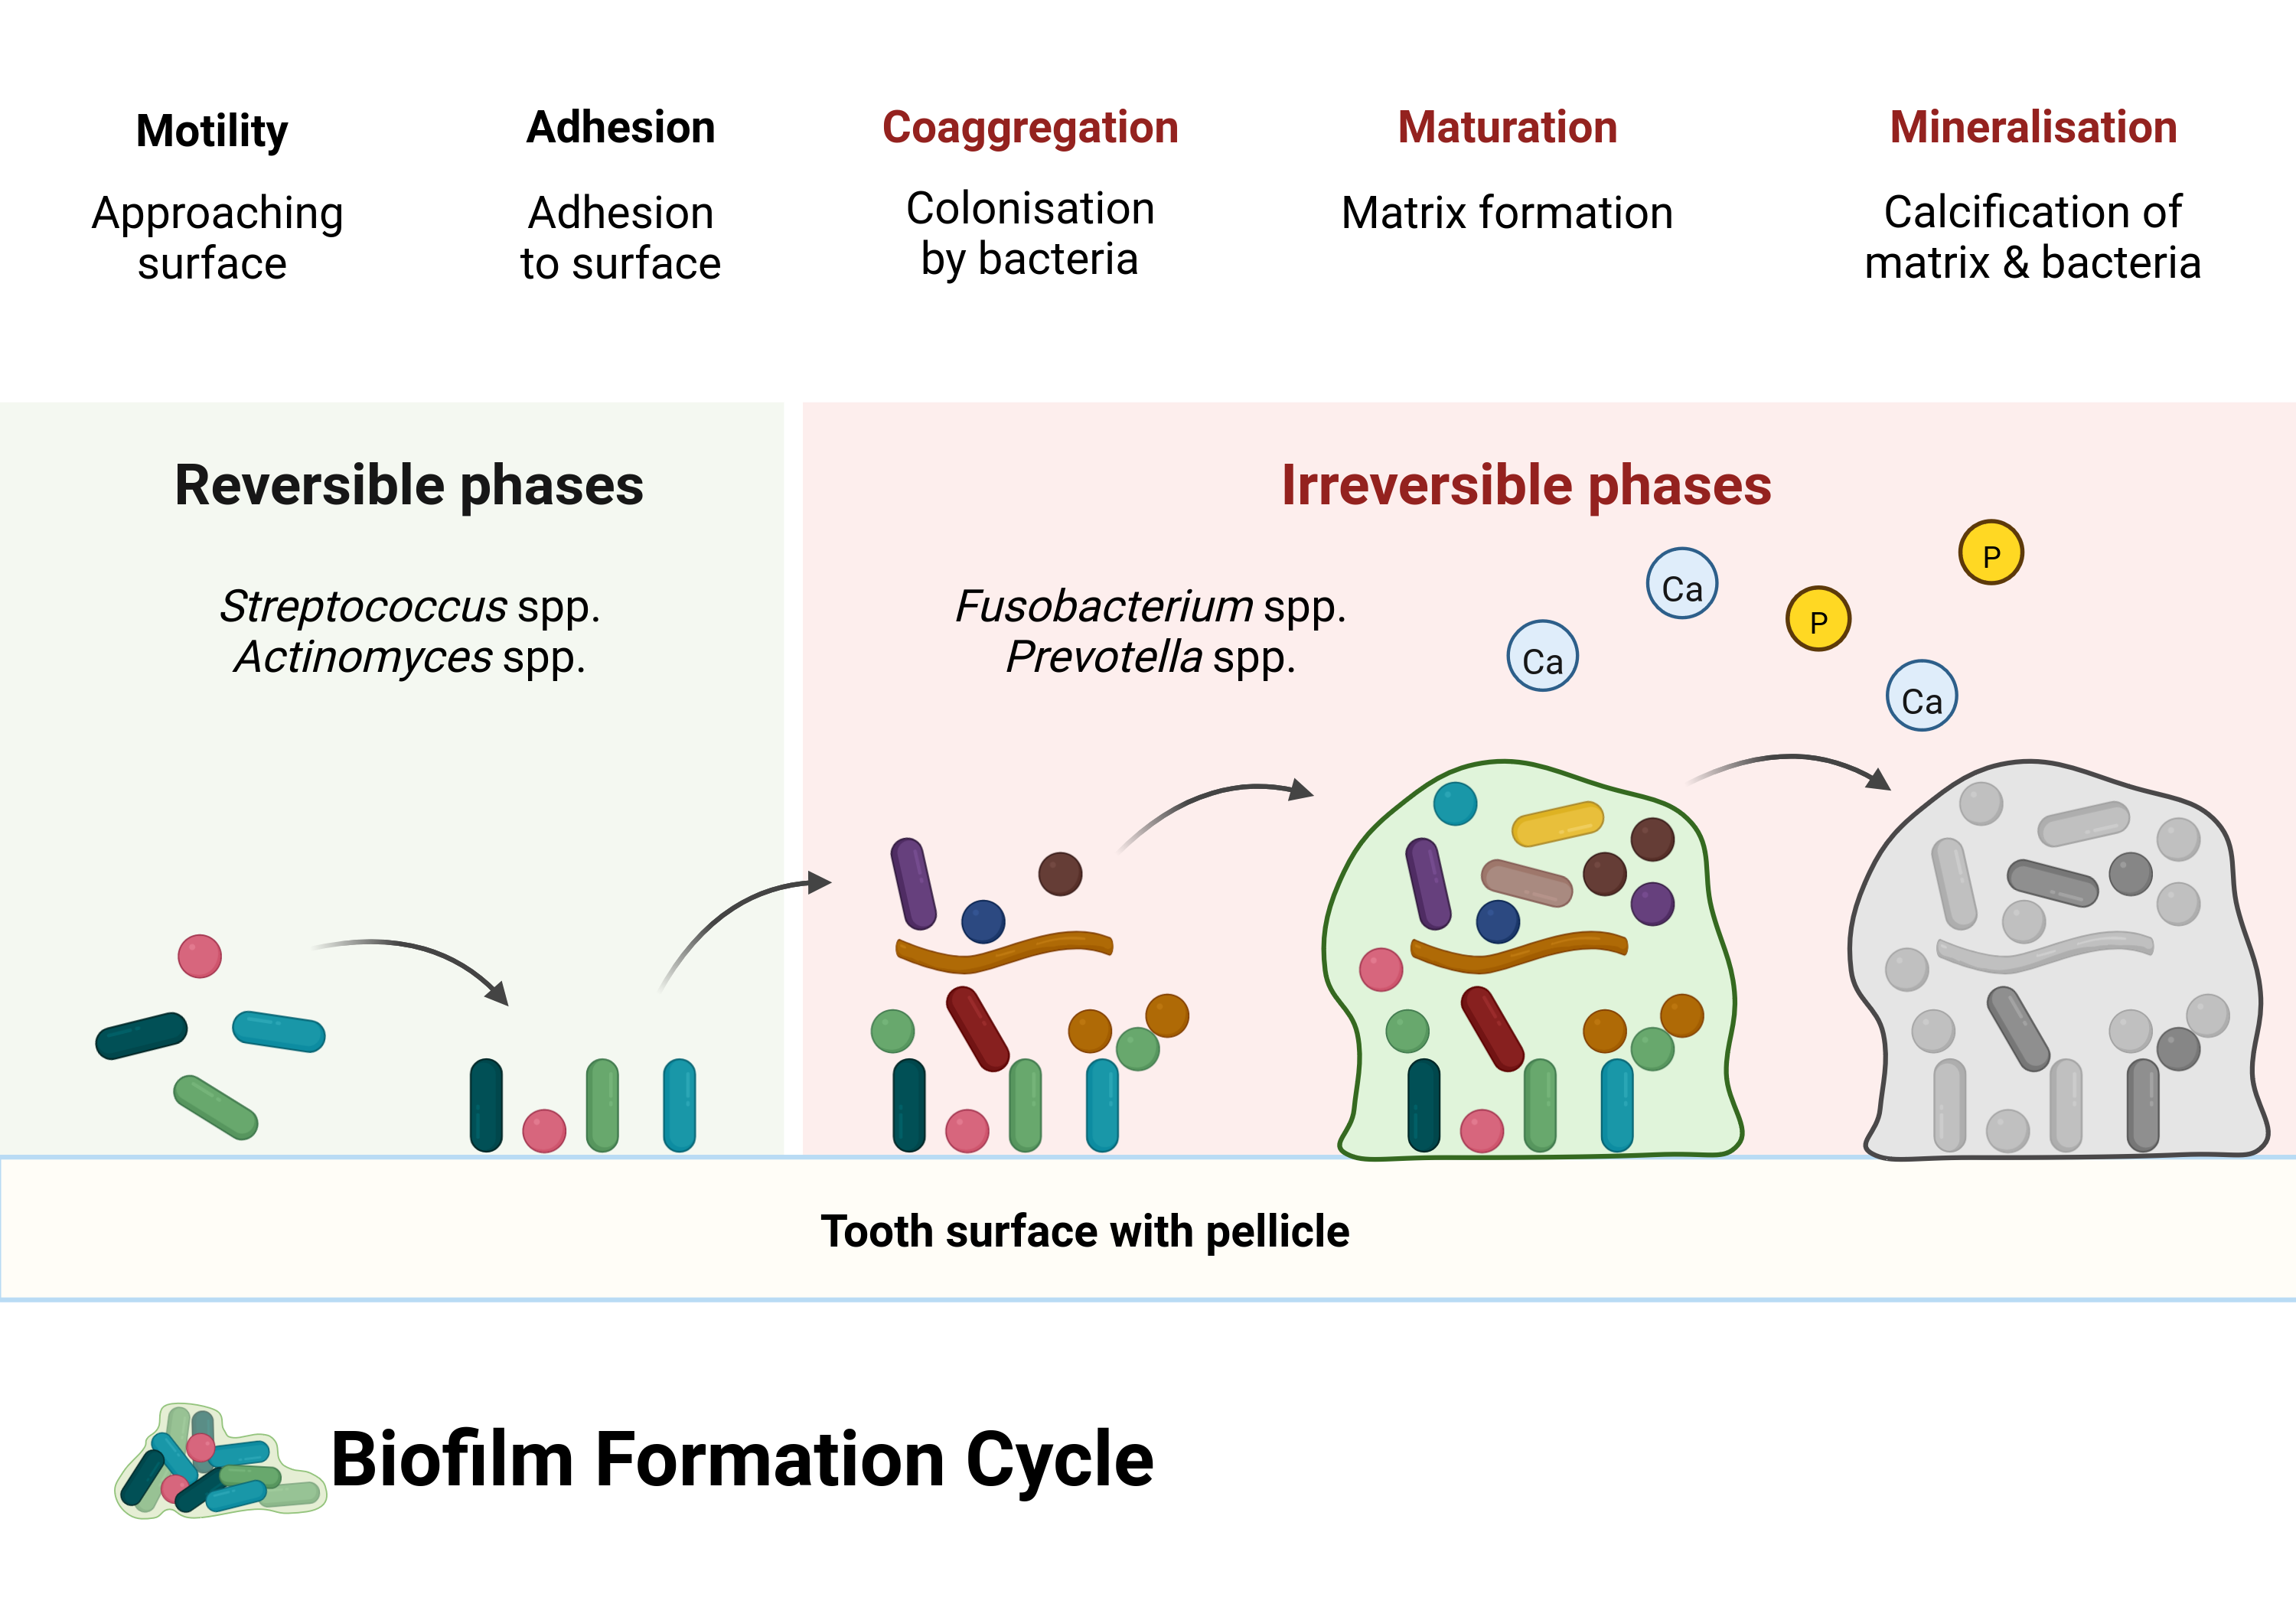
\includegraphics{./figures/biofilm_formation.png}

}

\caption{\label{fig-biofilm-form}A simplified overview of biofilm
formation. Created with BioRender.com. Still under construction.}

\end{figure}

The pellicle contains molecules (known as adhesins) that enable specific
bacteria to attach to complementary receptors on the pellicle. So when
the pellicle adsorbs to the tooth, it becomes a surface for bacterial
attachment (Yao et al., 2003). The first bacteria to attach are known as
early coloniser bacteria (or pioneer colonisers) and include
\emph{Streptococcus} species (spp.), \emph{Actinomyces} spp., and
\emph{Haemophilus} spp (Uzel et al., 2011; Zijnge et al., 2010). The
initial attachment occurs when the random movement of bacteria and the
flow of saliva brings them close enough to the pellicle to attach. Some
bacteria have a limited, often random, ability to move if they have long
tail-like structures known as flagella, but most are brought to the
surface by saliva.

As bacteria approach the pellicle-coated surface of a tooth, there are
both attractive and repulsive forces at work. Repulsion because both the
bacteria and pellicle proteins have a net negative charge (Song et al.,
2015), causing eloctrostatic repulsive force; and attraction from van
der Waals forces. Bacteria may be more or less likely to attach
depending on the distance from the bacteria to the surface. If the
bacteria come too close to the surface, the initial attraction (primary
maximum) will most likely be overcome by repulsion (primary maximum).
Bacteria are more likely to attach when they encounter attractive forces
at a further distance (secondary minimum), ultimately leading to a game
of `will-they-won't-they' between the bacteria and pellicle. This
initial attachment is a weak physicochemical long-distance (10--20 nm;
it's a long distance for bacteria) attraction; therefore, attachment is
initially reversible, as bacteria can become detached by salivary flow
or shearing action by the tongue (Philip D. Marsh et al., 2016). This
model of bacterial attachment, also known as the DLVO theory, can
partially explain the aspects involved in microbial adhesion. Further
explanation includes hydrodynamic forces, where hydrophobic components
of the pellicle and cell surface interact (Bos, 1999; Vigeant et al.,
2002). Overcoming the repulsive forces may be in part facilitated by
motility in some organisms. The aforementioned flagellum, for example,
may give the necessary `push' to reach a region of net attractive forces
(Jin \& Yip, 2002). Additionally, the ionic strength of saliva may play
a role in reducing electrostatic repulsion with increasing ionic
strength (Renner \& Weibel, 2011).

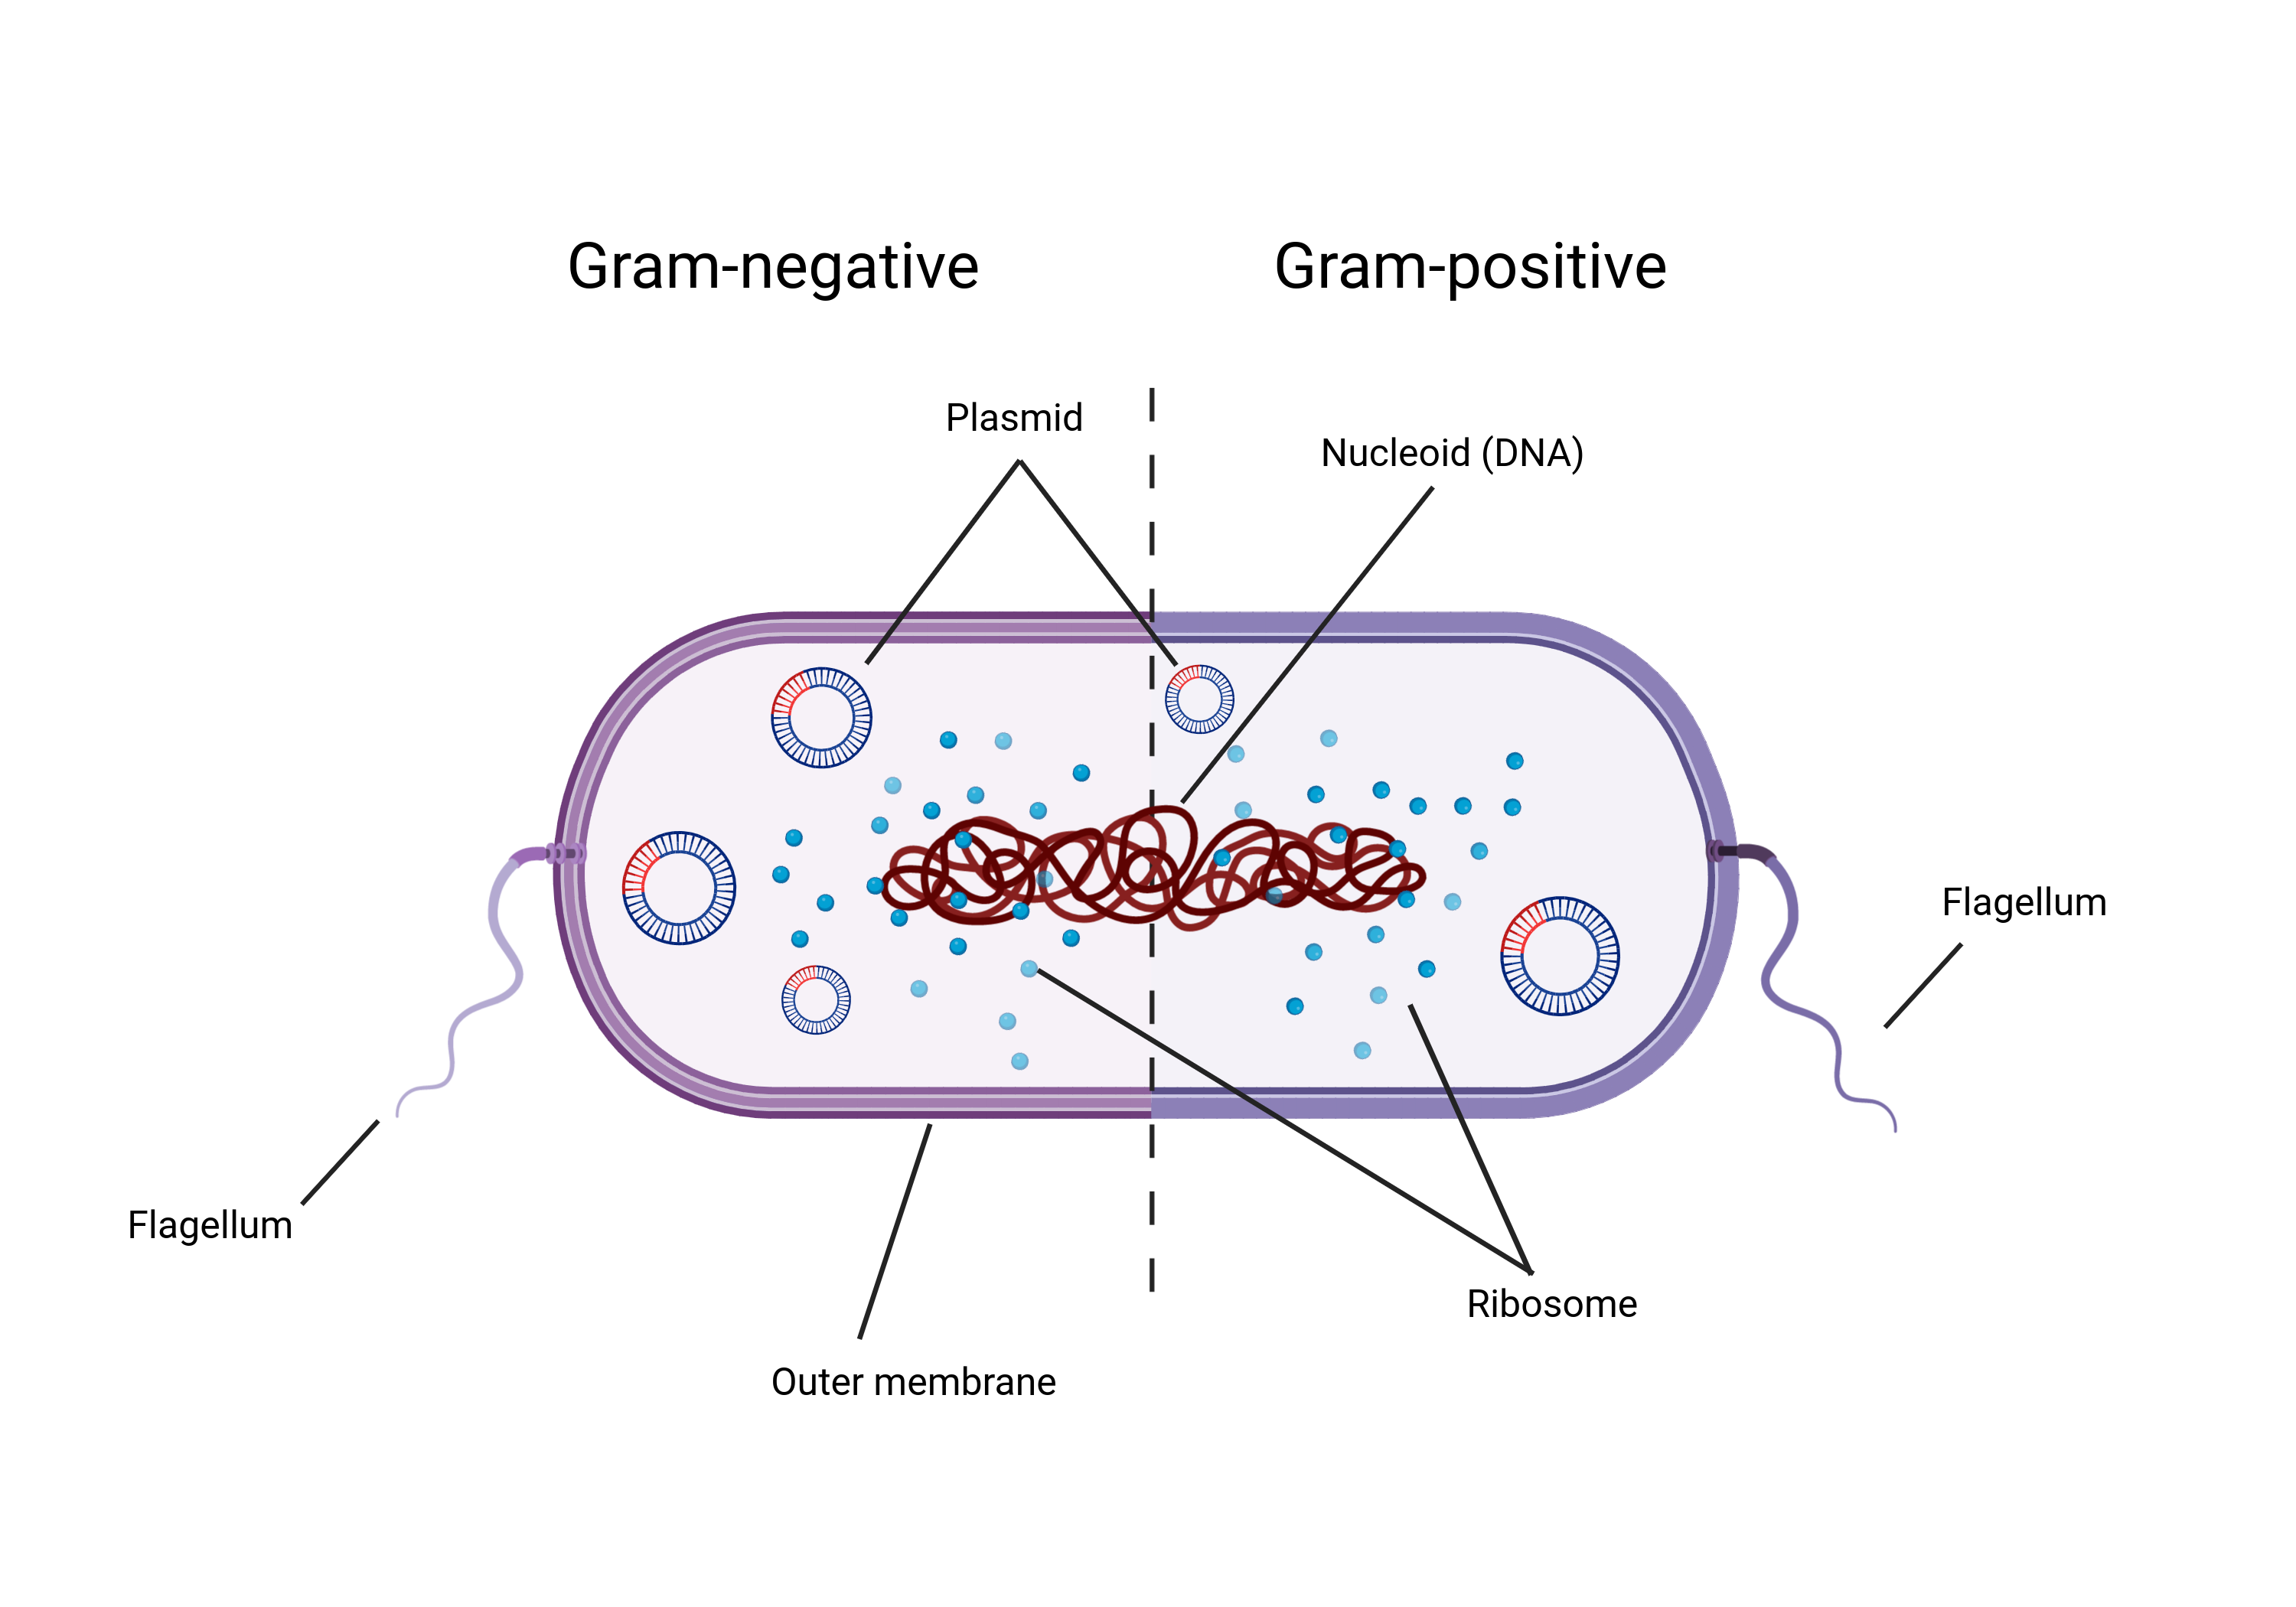
\includegraphics{figures/bacterial-structure.png}

Attachment becomes stronger and colonisation becomes more solidified at
a shorter distance, as surface molecules on the bacteria interact with
complementary receptors on the pellicle, and the interactions between
bacteria and pellicle become more direct. Some bacteria have components
on their surface that allow them to attach directly to complementary
components on the dental pellicle (adhesin-receptor interactions). These
attachments are very specific because only certain bacteria have the
right molecules on their surface (Jin \& Yip, 2002). These receptors are
often carbohydrates formed by the host, meaning us. Early colonisers are
also able to attach to proteins and enzymes present in saliva, as well
as onto the surface of other bacteria already attached to the pellicle
(Jin \& Yip, 2002; Nikitkova et al., 2013). When bacteria come within a
shorter distance of the pellicle they may also attach directly to the
surface with other hair-like structures (fimbriae) that are present on
the surface of some bacteria. These hair-like structures attach to
matching receptors that are present in the pellicle (Nobbs et al.,
2009).

While some bacteria specialise in attaching to surfaces, not all of them
possess this ability. However, once the specialists have attached, they
facilitate the adhesion of other bacteria (secondary colonisers) by
allowing them to attach to their surface (coadhesion) rather than
directly to the pellicle. For example, \emph{S. gordonii} can attach to
the pellicle and facilitate coadhesion with \emph{A. naeslundii} (Robert
J. Palmer Jr. et al., 2003). Not all attachments involve proteins. They
can also involve carbohydrates, enzymes, and various appendages on the
surface of the bacteria, although these appendages often consist of
proteins in their structure, for example the already mentioned pili and
fimbriae (Nobbs et al., 2009). This can occur on a large scale, causing
the number and types of bacteria on the tooth surface to grow, due to
the ability of different species to attach to one another
(coaggregation) (Jin \& Yip, 2002; Philip D. Marsh, 2006). Coaggregation
and coadhesion is an important part of the growing oral biofilm. Most
taxa don't have the necessary morphology to attach directly to a
substrate, however most oral taxa CAN coaggregate with other species
through cell-cell interactions, usually involving polysaccharides on the
bacterial-cell surfaces (Kolenbrander et al., 2010; Robert J. Palmer et
al., 2017).

As the biofilm formed by early colonisers grows through continued
multiplication and coadhesion/coaggregation, the diversity of the
biofilm increases. The proportion of early-colonising streptococci
gradually decreases while there is an increase of \emph{Tannerella
forsythia} \emph{Actinomyces} spp. and \emph{Fusobacterium nucleatum}
(Zijnge et al., 2010). \emph{F. nucleatum} is a bacterium also known as
the `bridging species', as it's believed to play an important part in
linking together early and late coloniser species---including
\emph{Prevotella} spp., \emph{S. gordonii}, and \emph{Porphyromonas
gingivalis}--- which might not otherwise be able to coaggregate
(Kolenbrander et al., 2010; Kolenbrander \& London, 1993). The
increasing diversity of bacteria adhering to a surface results in
communities of bacteria with the ability to communicate with each other,
distribute nutrients, and alter the local environment for more
favourable conditions. This is made possible by the presence of an
extracellular matrix, formed by the production of polymers by certain
bacterial species (Philip D. Marsh, 2010). Microenvironmental changes
can allow species to survive in otherwise unfavourable environments; for
example, the survival of many obligate anaerobes in an environment which
is largely aerobic (oxygen continuously enters the oral cavity as we
breathe). Bacteria with the ability to consume oxygen and produce carbon
dioxide allow bacteria with a lower oxygen tolerance to thrive (Philip
D. Marsh, 2005). In fact, dental plaque predominantly consists of
obligate and facultative anaerobes and is especially true for
periodontitis-associated biofilms, which tend to be dominated by more
species with a lower oxygen tolerance than their non-periodontitis
counterparts (Curtis et al., 2020). A pH balance may be maintained by
species that are able to consume acidic metabolic products produced by
other species, and convert them to weaker acids. \emph{Veillonella} spp.
especially (Philip D. Marsh, 2005). Metabolic products of some bacteria
are used by others as nutrients. By-products of urea metabolism can be
used by some organisms, who further break down the by-products, which
can be used by yet other organisms (Flemming et al., 2016). Working as a
community can increase survivability in the harsh and dynamic
environment of the oral cavity, with rapid changes in pH, oxygen,
nutrient availability, etc.

Perhaps ironically, an important part of the maturation of a biofilm is
the removal of bacteria from the biofilm itself. Removal can occur
through both internal and external mechanisms. It's likely that there is
a continuous loss of microbes near/on the surface of the biofilm caused
by shear forces from saliva and mechanical removal by the tongue. There
can be multiple motivating factors involved in the active detachment by
bacteria, including increasingly adverse conditions within the biofilm,
such as nutrient depletion or an unfavourable local environment. If
sufficiently adverse conditions persist, certain bacteria may make the
active decision to `peace out'. Dispersion of bacteria from a biofilm
requires production of matrix-degrading enzymes, and, as such, not all
bacteria can actively disperse from a biofilm (Petrova \& Sauer, 2016).
The detached bacteria then colonise other parts of the biofilm, making
the biofilm a highly dynamic structure undergoing continuous remodelling
(Flemming et al., 2016).

So far, the picture of biofilm formation is one of peaceful
coexsistance, collaboration, and even neighbourly interspecies actions.
A basis for this cooperation is increased overall benefits to the
communities (Rendueles \& Ghigo, 2015). However, competition between
bacteria still exists within the biofilm. The metabolic by-products
produced by some bacteria may be toxic for others, allowing the
producers to gain a competitive advantage. The aforementioned
acid-production by some bacteria can cause unfavourable conditions for
species that prefer more neutral pH environments, particularly in the
absence of the secondary feeders that would normally neutralise these
compounds. A more direct example of bacterial competition is the ability
of bacteria to produce substances that are toxic to other bacteria.
These are often proteins or peptides termed bacteriocins, and can either
inhibit or even kill other bacteria (Daw \& Falkiner, 1996; Graham et
al., 2017). \emph{S. sanguinis} and \emph{S. gordonii} can produce
H\textsubscript{2}O\textsubscript{2} that is toxic to \emph{S. mutans},
a member of their own genus. \emph{S. mutans} can, in turn, produce
mutacin, which inhibits the growth of \emph{S. sorbrinus}. There is no
love lost among these close relatives (P. Chen et al., 1999). In
addition to H\textsubscript{2}O\textsubscript{2}, oral streptococci can
produce lactate by consuming carbohydrates, giving them a competitive
advantage over acid-sensitive species by altering the local environment.
Some species are resistant to specific metabolic by-products that others
consider toxic, and may even consider them a delicacy (so to speak).
\emph{Veillonella} spp. are an example of organisms that thrive under
these conditions, allowing both streptococci and \emph{Veillonella} spp.
to accumulate in the biofilm and create a favourable environment to
select species (Edlund et al., 2018). These are simplistic examples, and
often competition involves more interactions between multiple species
taking on various roles of `sensing', `mediating', and `killing'
(Rendueles \& Ghigo, 2015). Competition between and within species will
ultimately shape the wider biofilm communities.

\hypertarget{dental-calculus}{%
\subsection{Dental calculus}\label{dental-calculus}}

The exact mechanism of dental calculus formation is not fully
understood, but involves processes of biomineralisation and crystal
formation within dental plaque. The main mineral components of calculus
are crystals containing various combinations of calcium and phosphate
ions. Other salts are also present, but the bulk of the crystals are
made up of calcium phosphates. Initial mineralisation of dental plaque
is a chemical process in which equilibrium of minerals in saliva and
gingival crevicular fluid tips towards saturation with regard to calcium
and phosphate, causing an increase of precipitation relative to
dissolution. This means, that when the concentration of ions increases
and tips the balance between dissolution and precipitation, salts will
accumulate within and on the surface of the biofilm. An increase in
concentration of minerals within the biofilm reaches a critical
threshold (supersaturation) and nucleation is triggered within the
plaque matrix, initiating crystal growth. This may or may not involve
spontaneous (or homogenous) nucleation, as it's unclear whether mineral
concentrations are sufficient to cause spontaneous nucleation, or
whether other biochemical processes act as a catalyst (Omelon et al.,
2013). That it's a chemical process can be shown by the ability to
produce calculus deposits in germ-free rats (Glas \& Krasse, 1962;
Theilade et al., 1964). Although it's unclear how the germ-free calculus
compares to conventional calculus, and, to my knowledge there have only
been studies on rats. Just because calculus growth can be induced in
sterile conditions, doesn't mean bacteria are non-essential to the
process. Bacteria are inevitably part of the scaffolding of dental
calculus in humans, since, as I mentioned in the beginning of this
chapter, our mouths are full of bacteria, and dental plaque is
essentially built by bacteria. Mineralisation does seem to start in the
biofilm matrix between microorganisms, but they are eventually also
mineralised along with the biofilm matrix (Friskopp, 1983). There are
pockets of living bacteria within dental calculus. These pockets and the
layer of plaque that covers the surface of dental calculus are likely
what cause the correlation between calculus presence and periodontal
disease (B. T. K. Tan, Mordan, et al., 2004). While the process can be
explained by chemistry, the conditions leading up to and surrounding the
process are both chemical and biological in nature, and certainly
involve bacteria. The main source of minerals in the oral cavity is
saliva, which enters the mouth through salivary glands. The three main
paired glands are the parotid, sublingual, and submandibular glands,
located by the cheeks, under the tongue, and under the lower jaw bone,
respectively. Saliva contains sodium (Na), potassium (K), calcium (Ca),
chlorine (Cl), bicarbonate (buffer), and inorganic phosphate (Pi)
(Dawes, 1970; Michael W. J. Dodds et al., 2005), and the locations of
the glands contribute to the pattern of dental calculus deposits within
the mouth, which commonly grow on the buccal portion of maxillary
(upper) molars and the lingual portion of mandibular (lower) incisors
(Jin \& Yip, 2002; D. J. White, 1997). Salivary pH also affects
saturation of salts, which in turn is influenced by salivary flow rates.
Increased flow rate of saliva will increase salivary pH, which reduces
dissolution and increases precipitation of calcium and phosphate. This
is an important mechanism that protects our teeth against
demineralisation of the enamel caused by caries. Protection is provided
by the exchange of calcium and phosphate from saliva to enamel (Dahlén
et al., 2010). Saliva further acts as a buffer for the oral cavity,
reducing the impact of short-term drops in pH caused by metabolic
byproducts of acid-producing bacteria (Michael W. J. Dodds et al., 2005;
Jin \& Yip, 2002). Higher rates of salivary flow are also likely to
contribute to an increase in calcium and phosphate secretion in addition
to pH, all contributing to an environment favouring plaque
mineralisation. Metabolic byproducts produced by bacteria can also
affect local pH, both pushing towards alkaline conditions as well as
acidic. A major cause of acidic pH is metabolism of overabundant dietary
sugars and starch, especially the metabolic activity of
\emph{Streptococcus mutans}, known to be one of the main culprits behind
dental caries (Bowen et al., 2018; Duarte et al., 2008; Exterkate et
al., 2010).

Conversely, alkaline conditions can be generated by metabolism of
various products that can either be directly or indirectly linked to
diet. One such product is urea. Urea is present in saliva, and its
concentration depends on multiple factors. One of these factors is a
high-protein diet, which increases levels of urea in serum and saliva
(Lieverse, 1999). Hydrolysis of urea produces ammonia and causes a rise
in pH. Bacteria possess the ability to produce ammonia from urea, which
is further used by ammonia-oxidising organisms and converted to nitrite
(Flemming et al., 2016; Sissons et al., 1994; Wong et al., 2002). In a
similar way, arginine can be broken down to ammonia and increase in pH.
Extended fluctuations in environmental conditions can alter the
composition of biofilms (X. Huang et al., 2012; Xuelian Huang et al.,
2017). Another pathway to alkalinity is through enzymatic activity.
Saliva contains proteases which specialise in breaking down proteins
into smaller components such as ammonia, and increased protease activity
in saliva may therefore cause an increase in calculus production (Jin \&
Yip, 2002).

There are also a number of inhibitors and promoters of mineralisation
present in the oral cavity, originating both from saliva and bacteria.
Substances known to promote plaque mineralisation through hydroxyapatite
formation and deposition, calcium-phospholipid-phosphate complexes
(CPLX), are present in bacteria. \emph{Corynebacterium matruchotii}
(formerly \emph{Bacterionema matruchotii}) accumulates calcium within
its cell structure, and has therefore received a lot of attention in
biomineralisation studies Ennever \& Creamer (1967). Biomineralisation
is not a feature unique to \emph{Corynebacterium matruchotii}. Even
species associated with caries may induce calcification under the right
conditions and after cell death (Moorer et al., 1993; Sidaway, 1978).
Inhibitors of biomineralisation include salivary proline-rich
polypeptides, small amino acids important for the immune system; and
statherin, a protein that controls the precipitation of calcium
phosphate in saliva (Jin \& Yip, 2002).

It's likely that multiple biomineralisation events occur under various
conditions, resulting in a heterogenous calculus composition with
crystals of various stages of growth (Friskopp, 1983; Friskopp \&
Hammarström, 1980). The differing susceptibility of bacteria to
calcification is also a contributor the heterogenous composition.
Overall, plaque mineralisation is a complex interaction between
conditions in the local environment, availability of minerals, the
equilibrium between precipitation and dissolution, balance between
nucleation promoters and inhibitors.

\hypertarget{oral-biofilm-models}{%
\section{Oral biofilm models}\label{oral-biofilm-models}}

Biofilm models are a way of studying the growth and development of
biofilms. By creating models that replicate the conditions and
complexity (to some extent) of biofilms in a lab, models allow
researchers to conduct various experiments to test the efficacy of
treatments on the growth and pathogenicity of biofilms. There are many
choices to be made when growing a biofilm, such as the composition of
the initial oral microbial community, nutrient content and availability,
and the makeup of the atmosphere {[}surrounding{]} the model. As such,
biofilm models can differ widely in their complexity and ability to
mimic conditions in a human mouth. A choice of model can be made based
on the end-goals of the research, or in some cases the choice is made
for you based on (a lack of) available equipment and financial
constraints. All models must have a defined biome containing a
substratum and nutrients. The substratum is a surface on which the
biofilm is intended to form and grow. For oral biofilm models the
environment is the oral cavity and the substrata are the teeth, tongue,
mucosa, or whatever the model isthe biofilm supposed to be mimicing. The
simplest models generally involve multiwell plates (e.g., 6-, 24-, and
98-well plates) with a substratum, usually glass cover-slips or
hydroxyapatite discs, placed at the bottom of the well. Similar models
suspend the substrata from a lid to promote active attachment of
bacteria to the substrata (Exterkate et al., 2010). When the substrata
are attached to a lid instead of the multiwell plates, it allows samples
to be periodically transferred between solutions/media if necessary,
adding more flexibility to the experimental setup.

Next, an inoculate is chosen. This can be anything from a single species
of bacterium (pure culture), to multiple select species (defined
consortium), to all organisms occurring naturally within a system
(microcosm) (McBain, 2009). The purpose of the incoulate is to initiate
biofilm formation by allowing the bacteria to adsorb to the substrata,
ideally in the presence of a conditioning film, such as saliva. For pure
cultures and defined consortia, the inoculate may come from saliva or
another oral site, such as dental plaque. The bacteria of interest are
then isolated using selective media, essentially providing ideal growing
conditions to certain types of bacteria, promoting their growth and
eliminating others (e.g. Basson \& van Wyk, 1996). Alternatively, the
bacteria can be acquired directly from companies like the American Type
Culture Collection (ATCC). For microcosms, the inoculate is often the
saliva itself, or dental plaque, in its (mostly) raw form. The inoculate
is added to the wells to initiate biofilm formation on the substrata as
described \protect\hyperlink{dental-plaque}{above}. As such, the content
of the inoculate influences the complexity of the biofilm microbiome as
well as the interactions between the communities within the biofilm
(Røder et al., 2016). It's not always possible to use donated saliva as
a growth medium for the duration of the experiment. Especially if the
experiment lasts more than a few days. Media containing salivary
components may be added for extended experiments. There are many
different recipes for media floating around out there, but most of them
are generally a mixture containing mucin, proteins, minerals commonly
found in saliva, and a buffer to maintain pH (Exterkate et al., 2010;
Pratten et al., 1998; Shellis, 1978; Sissons et al., 1991; Tian et al.,
2010).

More complicated models make use of increasingly sophisticated equipment
to mimic the oral environment. Another level of model complexity can be
added by adjusting the rate at which nutrients are dispersed through the
system, and the overall nutrient supply. Nutrient distribtion can be
continuous, semi-continuous, or batch cultures, with the latter
providing a finite amount of nutrients in a closed system. An example of
a batch culture model is a biofilm grown on an agar plate, which has a
finite amount of resources (Kearns et al., 2005). Once the nutrients in
the agar have been depleted, that's it. At the other end of the spectrum
is a system with a pump attached to a reservoir that can continuously
supply the biofilm with growth medium, similar to salivary flow. In
between the former options is the semi-continuous supply of nutrients.
This can, for example, be the multiwell plate model with a lid, where
the samples can be periodically transferred to new plates containing
fresh growth medium (Exterkate et al., 2010). Other parameters that can
be controlled to more closely simulate conditions in the oral cavity are
pH and gas phase, as can be done with the multistation artificial mouth
(MAM). The MAM gives researchers control over a large number of
parameters using multiple chambers with complete control over the flow
of treatment and/or nutrient conditions---environmental conditions such
as pH, temperature, and gas phase---and access to real-time measurements
(Sissons, 1997).

The duration of an experiment depends on the scope of the study. If the
purpose is to learn more about initial biofilm formation and prevention,
it may only be necessary to grow the biofilms for a few hours to 48
hours (Dibdin, 1981; Exterkate et al., 2010). If, instead, the goal is
to learn more about biofilm maturation and calcification, the
experiments can run for days or even weeks (Sara K. Filoche et al.,
2007; Sissons et al., 1991; Wong et al., 2002).

Models developed for studying oral biofilms include, in increasing
complexity, the ACTA active attachment (AAA) model (Exterkate et al.,
2010), Calgary biofilm device (Ceri et al., 1999), modified Robbins
device (MRD) (Honraet \& Nelis, 2006), constant depth film-fermenter
(CDFF) (Peters \& Wimpenny, 1988), and the multistation artificial mouth
(MAM) (Sissons et al., 1991) representing the upper echelon of
complexity. Summaries of biofilm models, including benefits and
limitations of the various types, can be found in reviews by McBain
-McBain (2009), Tan and colleagues -C. H. Tan et al. (2017), and Røder
and colleagues -Røder et al. (2016).

It might be tempting to think that the goal should always be to mimic
the oral environment as closely as possible. However, there are benefits
to more simplistic models, as well as limitations to the more
sophisticated models. Benefits of pure cultures and defined consortia
are reproducibility between experiments and more control over
physiological and factors and making it easier to take various
measurements. Microcosms have the benefit of more closely mimicking the
complexity of the organisms' natural environment (McBain, 2009).
However, even microcosms can be limited in their ability to recreate the
complexity and diversity of the oral microbiome (Tian et al., 2010).
Alternatives to \emph{in vitro} models are \emph{in situ} models which
usually involve growing plaque on a removable surface inside a the mouth
of a willing participant. These models add a level of realism, as they
are grown inside an actual oral cavity, and can reflect biogeographical
differences in biofilm composition caused by differing conditions across
the oral cavity. They also come with additional difficulties and reduced
control over experimental parameters (P. D. Marsh, 1995; Zero, 1995).

\bookmarksetup{startatroot}

\hypertarget{byoc-valid}{%
\chapter{Assessing the validity of a calcifying oral biofilm model as a
suitable proxy for dental calculus}\label{byoc-valid}}

\hypertarget{introduction}{%
\section{Introduction}\label{introduction}}

Dental calculus is becoming an increasingly popular substance for
exploring health and diet in past populations (Warinner et al., 2015).
During life, dental plaque undergoes periodic mineralisation, trapping
biomolecules and microfossils that are embedded within the dental plaque
biofilm in the newly-formed dental calculus. This process is repeated as
new plaque is deposited and subsequently mineralises, resulting in a
layered structure representing a temporal record of biofilm growth and
development (Warinner, Rodrigues, et al., 2014). The calculus serves as
a protective casing for the entrapped biomolecules and microfossils,
preserving them for thousands of years after death and burial (Fellows
Yates et al., 2021). Studies using archaeological dental calculus span a
wide range of topics in different regions and time periods. These
include characterisation of the oral microbiome and its evolution in
past populations (Adler et al., 2013; Fellows Yates et al., 2021;
Kazarina et al., 2021; Velsko et al., 2019; Warinner, Rodrigues, et al.,
2014), as well as extraction of microbotanical remains (Hardy et al.,
2009; Henry \& Piperno, 2008; Ma et al., 2022; Mickleburgh \&
Pagán-Jiménez, 2012) and other residues to infer dietary patterns and
nicotine use (Bartholdy, Hasselstrøm, et al., 2023; Buckley et al.,
2014; Eerkens et al., 2018; Hendy et al., 2018; Velsko, Overmyer, et
al., 2017). Dental calculus has already provided a unique and valuable
insight into the past, but the exact mechanism of the incorporation,
retention, and preservation of microfossils and biomolecules exogenous
to the microbial biofilm is largely unknown; even the process of plaque
mineralisation is not fully understood (Jin \& Yip, 2002; Omelon et al.,
2013). This means that there may be hidden biases affecting our
interpretations of dietary/activity patterns extrapolated from ancient
dental calculus. These biases have been explored archaeologically
(Fagernäs et al., 2022; Tromp et al., 2017) as well as in contemporary
humans (Leonard et al., 2015) and non-human primates (R. C. Power et
al., 2015), but not experimentally.

Dental plaque is an oral biofilm and is part of the normal state of the
oral cavity. However, when left unchecked, plaque can lead to
infections, such as dental caries and periodontitis, and/or
mineralisation (Philip D. Marsh, 2006). The dental plaque biofilm grows
in a well-characterized manner before mineralisation, in a process that
repeats regularly to build up dental calculus. Shortly after teeth are
cleaned (whether mechanically or otherwise), salivary components adsorb
to the crown or root and form the acquired dental pellicle. The pellicle
provides a viable surface for bacteria to attach, especially
early-coloniser species within the genera \emph{Streptococcus} and
\emph{Actinomyces} (Philip D. Marsh, 2006). Once the tooth surface has
been populated by specialists in surface-attachment, other species of
bacteria can attach to the adherent cells, increasing the biofilm
density and diversity. The bacterial species secrete polysaccharides,
proteins, lipids, and nucleic acids, into their immediate environment to
form a matrix that provides structural support, nutrition, and allows
for environmental niche partitioning (Flemming et al., 2016).

Biofilms can become susceptible to calcification under certain
microenvironmental conditions, including an increased concentration of
salts and a decrease in statherin and proline-rich proteins in saliva,
rises in local plaque pH, and increased hydrolysis of urea (D. J. White,
1997; Wong et al., 2002). These conditions can cause increased
precipitation and decreased dissolution of calcium phosphate salts
within saliva and the plaque biofilm. The resulting supersaturation of
calcium phosphate salts is the main driver of biofilm mineralisation
(Jin \& Yip, 2002). The primary minerals in dental calculus are
hydroxyapatite, octacalcium phosphate, whitlockite, and brushite. During
initial mineralisation the main mineral component is brushite, which
shifts to hydroxyapatite in more mature dental calculus (Hayashizaki et
al., 2008; Jin \& Yip, 2002). The exact elemental composition of dental
calculus varies among individuals due to various factors, including diet
(Hayashizaki et al., 2008; Ji et al., 2000).

Dental plaque can also be grown \emph{in vitro}, and these oral biofilm
models are commonly used in dental research to assess the efficacy of
certain treatments on dental pathogens (Exterkate et al., 2010; S. K.
Filoche et al., 2007) without the ethical issues of inducing plaque
accumulation in study participants and the complexity of access and
sampling in humans or animals. Oral biofilm models are often short-term
models grown over a few days, but longer term models also exist (up to
six weeks) which are used to develop mature plaque or dental calculus
(J. D. Middleton, 1965; Sissons et al., 1991; Velsko \& Shaddox, 2018;
Wong et al., 2002). A well-known limitation of biofilm models is the
difficulty in capturing the diversity and complexity of bacterial
communities and metabolic dependencies, micro-environments, nutrient
availability, and host immune-responses in the natural oral biome
(Bjarnsholt et al., 2013; Edlund et al., 2018; Velsko, Cruz-Almeida, et
al., 2017; Velsko \& Shaddox, 2018). These limitations can be overcome
by complex experimental setups, but at the cost of lower throughput and
increased requirements for laboratory facilities.

Despite the limitations, oral biofilm models have many benefits over
\emph{in situ} research. There are many variables involved in dental
calculus formation, such as intra- and inter-individual variation in
salivary flow, oral pH, and amylase activity, which can be hard to tease
apart \emph{in situ}. Oral biofilm models provide a controlled
environment to explore the effect of selected variables on the growth of
calculus and the retention of dietary components in the biofilm, as well
as a means to identify how the methods used in archaeology may
inadvertently bias the interpretations. This type of research has, so
far, been limited, but has the potential to greatly benefit
archaeological research on past diet (Anita Radini \& Nikita, 2022).

We present an oral biofilm model that can serve as a viable proxy for
dental calculus for archaeology-oriented research questions. It is a
multispecies biofilm using whole saliva as the inoculate, with a simple
multiwell plate setup that is accessible even to smaller lab budgets and
those with limited facilities for microbiology work. Here, we used
next-generation sequencing and metagenomic classification to
characterise the bacterial composition of our model dental calculus and
compare it to oral reference samples, including saliva, buccal mucosa,
plaque, and modern human dental calculus. This was done to ensure that
the model microbiome is predominantly oral and not overgrown by
environmental contaminants. We then determined the mineral composition
of the model dental calculus using Fourier transform infrared (FTIR)
spectroscopy to verify the presence of calculus-specific mineral phases
and functional groups, and perform a qualitative comparison with modern
and archaeological reference calculus. Overall the model calculus is
chemically similar to natural calculus, and has a predominantly oral
microbiome. The microbial diversity and richness within the model
samples were lower than oral reference samples, suggesting that the
model samples do not contain identical species composition and
abundances as the natural samples. The mineral composition closely
resembles modern and archaeological reference calculus, predominantly
comprised of carbonate hydroxyapatite with a similar level of
crystallinity and order. As such, the model dental calculus presented
here is a viable proxy to natural dental calculus and can be used to
explore many of the currently unexplained processes we see in the
archaeological material, when working within the limitations of an oral
biofilm model.

\bookmarksetup{startatroot}

\hypertarget{investigating-biases-associated-with-dietary-starch-incorporation-and-retention-with-an-oral-biofilm-model}{%
\chapter{Investigating Biases Associated with Dietary Starch
Incorporation and Retention with an Oral Biofilm
Model}\label{investigating-biases-associated-with-dietary-starch-incorporation-and-retention-with-an-oral-biofilm-model}}

\bookmarksetup{startatroot}

\hypertarget{byocstarch-intro}{%
\chapter{Introduction}\label{byocstarch-intro}}

Dental calculus has proven to contain a wealth of dietary information in
the form of plant microfossils (Hardy et al., 2009; Henry \& Piperno,
2008), proteins (Hendy et al., 2018; Warinner, Hendy, et al., 2014), and
other organic residues (Buckley et al., 2014). This dietary information
can be preserved within the mineralised dental plaque over many
millennia, providing a unique window into the food-related behaviours of
past populations (Henry \& Piperno, 2008; Jovanović et al., 2021; Tao et
al., 2020) and extinct species (Hardy et al., 2012; Henry et al., 2014).

Until recently, only a few studies directly investigated the presence of
plant microremains in the dental calculus of archaeological remains. The
ability to extract phytoliths from the dental calculus of archaeological
fauna to investigate diet was first noted by Armitage (1975), and later
by Middleton and Rovner (1994), and Fox and colleagues (1996). Starches
and phytoliths were extracted from human dental calculus by Cummings and
Magennis (1997).\\
In more recent years, the study of dental calculus has increased
exponentially, and the wealth of information contained within the
mineralised matrix has largely been acknowledged. The use of dental
calculus spans a wide variety of archaeological research areas, such as
oral microbiome characterisation (including pathogens) through the
analysis of DNA and proteins (Adler et al., 2013; Warinner, Rodrigues,
et al., 2014), microbotanical remains (Hardy et al., 2009; Henry \&
Piperno, 2008; Mickleburgh \& Pagán-Jiménez, 2012), other organic
residues and proteins from dietary compounds (Buckley et al., 2014;
Hendy et al., 2018), and nicotine use (Eerkens et al., 2018). Especially
the extraction of starch granules has become a rich source of dietary
information, as starch granules have proven to preserve well within
dental calculus over a variety of geographical and temporal ranges
(Henry et al., 2014; Jovanović et al., 2021; Piperno \& Dillehay, 2008;
Tao et al., 2020).

Despite this, our knowledge of dental calculus and the incorporation
pathways of the various markers is limited (A. Radini et al., 2017), as
is our knowledge of information-loss caused by these pathways.
Additionally, the methods we use to extract and analyse dental calculus,
and make inferences on past diets represent another potential source of
bias. Studies on both archaeological and modern individuals have
explored these biases in more detail. Extraction methods were tested by
Tromp and colleagues (2017), specifically regarding decalcification
using HCl or EDTA. The authors found significantly more starches with
the EDTA extraction method than the HCl extraction method; however, as
noted by the authors, comparisons involving archaeological calculus are
problematic due to variability between and within individuals. Studies
conducted on modern humans (Leonard et al., 2015) and non-human primates
(R. C. Power et al., 2015; Robert C. Power et al., 2021) have explored
how well microremains (phytoliths and starches) extracted from dental
calculus represent the actual dietary intake. These studies are
justifiably limited, despite meticulous documentation and observation,
due to unknown variables and uncertainty involved in this kind of
\emph{in vivo} research. Dental calculus is a complex oral biofilm with
a multifactorial aetiology and variable formation rates both within and
between individuals (Haffajee et al., 2009; Jepsen et al., 2011),
contributing to the stochasticity of starch representation being
observed in numerous studies. Additionally, the concentration of oral
\(\alpha\)-amylase differs both between and within individuals
(Froehlich et al., 1987; Nater et al., 2005), causing different rates of
hydrolysis of the starch granules present in the oral cavity. Add to
this the effects of the many different methods of starch processing
(Hardy et al., 2018), as well as post-depositional processes that are
still being explored (García-Granero, 2020; Mercader et al., 2018), and
it becomes clear that using dental calculus to reconstruct diet is a
highly unpredictable process.

In this exploratory study, we use an oral biofilm model to investigate
the retention of starch granules within dental calculus in a controlled
laboratory setting, allowing us full control over dietary input. Our
main questions concern the representation of granules extracted from the
calculus compared to the actual intake. How much of the original diet is
incorporated into the calculus, and how much is recovered? Is there
differential loss of information from specific dietary markers that
affects the obtained dietary information, and how does this affect the
representation of diet from extracted microremains?\\
We find that, despite the absence of \(\alpha\)-amylase in the model, a
limited proportion of the starch input is actually retained in the
calculus. We also observed a shift in the size ratios of individual
starch granules that are incorporated into the calculus, and that the
number of incorporated starch granules increases as the size of the
calculus deposit increases.

\bookmarksetup{startatroot}

\hypertarget{materials-and-methods}{%
\chapter{Materials and Methods}\label{materials-and-methods}}

\hypertarget{biofilm-formation}{%
\section{Biofilm formation}\label{biofilm-formation}}

In this study we employ a multispecies oral biofilm model following a
modified protocol from Sissons and colleagues (1991) and Shellis (1978).
In brief, a biofilm inoculated with whole saliva was grown on a
substrate suspended in artificial saliva, and fed with sugar (sucrose).
After several days of growth, the biofilm was exposed to starch
solutions. Mineralisation of the biofilm was aided by exposure to a
calcium phosphate solution. After 25 days of growth, the mineralised
biofilm was collected for further analysis. The setup comprises a
polypropylene 24 deepwell PCR plate (KingFisher 97003510) with a lid
containing 24 pegs, which is autoclaved at 120°C, 1 bar overpressure,
for 20 mins. The individual pegs were the substrata on which the
calculus grew. Using this system allowed for easy transfer of the
growing biofilm between saliva, feeding solutions, and mineral
solutions.

The artificial saliva (AS) is a modified version of the basal medium
mucin (BMM) described by Sissons and colleagues (1991). It contains 2.5
g/l partially purified mucin from porcine stomach (Type III, Sigma
M1778), 5 g/l trypticase peptone (Roth 2363.1), 10 g/l proteose peptone
(Oxoid LP0085), 5 g/l yeast extract (BD 211921), 2.5 g/l KCl, 0.35 g/l
NaCl, 1.8 mmol/l CaCl\textsubscript{2}, 5.2 mmol/l
Na\textsubscript{2}HPO\textsubscript{4} (Sissons et al., 1991), 6.4
mmol/l NaHCO\textsubscript{3} (Shellis, 1978), 2.5 mg/l haemin. This is
subsequently adjusted to pH 7 with NaOH pellets and stirring, autoclaved
(15 min, 120°C, 1 bar overpressure), and supplemented with 5.8
\(\mu\)mol/l menadione, 5 mmol/l urea, and 1 mmol/l arginine (Sissons et
al., 1991).

Fresh whole saliva (WS) for inoculation was provided by a 31-year-old
male donor with no history of caries, who abstained from oral hygiene
for 24 hours. No food was consumed two hours prior to donation and no
antibiotics were taken up to six months prior to donation. The saliva
was filtered through a sterilised (with sodium hypochlorite, 10--15\%
active chlorine) nylon cloth to remove particulates. Substrata were
inoculated with 1 ml/well of a two-fold dilution of WS in sterilised
20\% (v/v) glycerine for four hours at 36°C, to allow attachment of the
salivary pellicle and plaque-forming bacteria. After initial
inoculation, the substrata were transferred to a new plate containing 1
ml/well AS and incubated in a shaking incubator (Infors HT Ecotron) at
36°C, 30 rpm. The inoculation process was repeated on days 3 and 5. AS
was partially refreshed once per day and fully refreshed every three
days, throughout the experiment, by transferring the substrata to a new
plate containing stock AS. To feed the bacteria, the substrata were
transferred to a new plate, containing 5\% (w/v) sucrose, for six
minutes twice daily, except on inoculation days (days 0, 3, and 5),
where the samples only received one sucrose treatment after inoculation.

Starch treatments were initiated on day 9 to avoid starch granule counts
being affected by \(\alpha\)-amylase hydrolysis from saliva inoculation
days. An \(\alpha\)-amylase (EC 3.2.1.1) activity assay was conducted to
confirm that no amylase was present in the model before starch
treatments started. Starch treatments replaced sucrose treatments,
occurring twice per day for six minutes. The starch treatments involved
transferring the substrata to a new plate containing a 0.25\% (w/v)
starch from potato (Roth 9441.1) solution, a 0.25\% (w/v) starch from
wheat (Sigma S5127) solution, and a 0.5\% (w/v) mixture of equal
concentrations (w/v) wheat and potato. All starch treatments were
created in dH\textsubscript{2}O with 5\% (w/v) sucrose. Before
transferring biofilm samples to the starch treatment plate, the plates
were agitated to keep the starches in suspension in the solutions.
During treatments, the rpm was increased to 60 to facilitate contact
between starch granules and biofilms.

After 15 days, mineralisation was encouraged with a calcium phosphate
monofluorophosphate urea (CPMU) solution containing 20 mmol/l
CaCl\textsubscript{2}, 12 mmol/l
NaH\textsubscript{2}PO\textsubscript{4}, 5 mmol/l
Na\textsubscript{2}PO\textsubscript{3}F, 500 mmol/l urea, and (0.04 g/l
MgCl) (Pearce \& Sissons, 1987; Sissons et al., 1991). The substrata
were submerged in 1 ml/well CPMU for six minutes, five times daily, in a
two-hour cycle. During the mineralisation period, starch treatments were
reduced to once per day after the five CPMU treatments. This process was
repeated for 10 days until the end of the experiment on day 24 (see
Figure @ref(fig:protocol-fig) for an overview of the protocol).

All laboratory work was conducted in sterile conditions under a laminar
flow hood to prevent starch and bacterial contamination. Control samples
that only received sucrose as a treatment were included to detect starch
contamination from the environment or cross-contamination from other
wells in the same plate.

\hypertarget{amylase-activity-detection}{%
\section{Amylase activity detection}\label{amylase-activity-detection}}

An \(\alpha\)-amylase (EC 3.2.1.1) activity assay was conducted on
artificial saliva samples collected from the plate wells on days 3, 6,
8, 9, 10, 12, and 14. Whole saliva samples were collected on days 0, 3,
and 5 as positive controls. Collected samples were stored at 4°C until
the assay was conducted on day 18. All samples and standard curves were
run in triplicates on two separate plates. Positive control saliva
samples were compared against a standard curve containing
H\textsubscript{2}O, while artificial saliva samples were compared
against a standard curve containing stock AS (due to the colour of
artificial saliva). Two photometric readings were conducted for each
plate with a 540 nm filter on a Multiskan FC Microplate Photometer
(Thermo Scientific 51119000). The protocol is a modified version of an
Enzymatic Assay of \(\alpha\)-Amylase
(\url{https://www.sigmaaldrich.com/NL/en/technical-documents/protocol/protein-biology/enzyme-activity-assays/enzymatic-assay-of-a-amylase})
(Bernfeld, 1955), which measures the amount of maltose released from
starch by \(\alpha\)-amylase activity. Results are reported in units (U)
per mL enzyme, where 1 U releases 1 \(\mu\)mole of maltose in 6 minutes.
The detailed protocol can be found here:
\url{https://www.protocols.io/view/amylase-activity-bw8jphun}.

\hypertarget{treatment-solutions}{%
\section{Treatment solutions}\label{treatment-solutions}}

A 1 ml aliquot of each starch solution was taken, from which 10 \(\mu\)l
was mounted on a microscope slide with an 18 x 18 mm coverslip, and
counted under a light microscope (Zeiss Axioscope A1). For wheat and
mixed treatment samples, we counted three slide transects (at ca. 1/4,
1/2, and 3/4 of the slide), and the sample counts were extrapolated to
the total number of granules exposed to the samples over 16 days of
treatments (see Supplementary Material for more details). For potato
treatment samples, the whole slide was counted.

\hypertarget{extraction-method}{%
\section{Extraction method}\label{extraction-method}}

Extraction of starches from the calculus samples was performed by
dissolving the calculus in 0.5 \(\tiny{M}\) ethylenediaminetetraacetic
acid (EDTA) (Le Moyne \& Crowther, 2021; Modi et al., 2020; Tromp et
al., 2017), and vortexing for 3 days until the sample was completely
dissolved. Twenty \(\mu\)l of sample was mounted onto a slide with an
18x18 mm coverslip. When transferring the sample to the slide, the
sample was homogenised using the pipette to ensure that the counted
transects were representative of the whole slide. The count from the
slide was extrapolated to the whole sample (see Supplementary Material
for more detail).

Both wheat and potato granules were divided into three size categories:
small (\textless10 \(\mu\)m), medium (10 -- 20 \(\mu\)m), and large
(\textgreater20 \(\mu\)m).

\hypertarget{statistical-analysis}{%
\section{Statistical analysis}\label{statistical-analysis}}

Statistical analysis was conducted in R version 4.3.0 (2023-04-21) (R
Core Team, 2020) and the following packages: tidyverse (Hadley Wickham
et al., 2019), broom (Robinson et al., 2021), here (Müller, 2020), and
patchwork (Pedersen, 2020).

To see if biofilm growth was differently affected by starch treatments,
a one-way ANOVA with sample weight as the dependent variable (DV) and
treatment as the grouping variable (GV) was conducted. To analyse
granule counts and calculate size proportions, mean counts for each
treatment were taken across both experimental plates, resulting in a
mean count for each granule size category within each treatment.

Pearson's \emph{r} was conducted on sample weight and total starch
count, as well as sample weight and starch count per mg calculus. The
total count for each sample within a treatment was standardised by
z-score to account for the differences in magnitude between the potato
and wheat counts. This was applied to total biofilm weight and starch
count per mg calculus (also z-score standardised) to account for
differences in starch concentration in the calculus (as per Wesolowski
et al., 2010).

\bookmarksetup{startatroot}

\hypertarget{results}{%
\chapter{Results}\label{results}}

All samples yielded sufficient biofilm growth and starch incorporation
to be included in the analysis (Figure @ref(fig:microscope-fig)),
resulting in a total of 48 biofilm samples (two plates of 24), 45 of
which were used for analysis (three samples were set aside for later
analysis). Most control samples contained no starch granules, while some
contained negligible quantities (see Supplementary Material).

\hypertarget{no-amylase-activity-detected-in-the-model}{%
\section{No amylase activity detected in the
model}\label{no-amylase-activity-detected-in-the-model}}

No \(\alpha\)-amylase activity was detected in any of the artificial
saliva samples from any of the days that were sampled. Only positive
controls (saliva) contained amylase activity that could be detected in
the assay, ranging from 9.93 to 30.2 U/mL enzyme (full results can be
found in the Supplementary Material). The results are not comparable to
other studies presenting \(\alpha\)-amylase activity levels in humans,
as the unit definition may differ; however, they are sufficient to show
that there is no activity in the model.

\hypertarget{treatment-type-had-minimal-effect-on-biofilm-growth}{%
\section{Treatment type had minimal effect on biofilm
growth}\label{treatment-type-had-minimal-effect-on-biofilm-growth}}

A one-way ANOVA suggests that the type of starch used during the biofilm
growth period had a minimal effect on the growth of the biofilm
(expressed as total dry weight of the sample), F(3, 43) = 1.16, p =
0.335. A summary of sample weights is available in Table
@ref(tab:anova-tbl).

\hypertarget{starch-counts}{%
\section{Starch counts}\label{starch-counts}}

It was not possible to differentiate between potato and wheat starches
smaller than ca. 10 \(\mu\)m. These were counted as wheat, as we assumed
that the majority of the small granules were wheat. We make this
assumption based on the counts of small starches in the wheat-only and
potato-only solutions. Of the combined amount of small starches in these
two solutions, 99.2\% are from wheat.

The separate wheat and potato solutions were made with a 0.25\% (w/v)
starch concentration, while the mixed-starch solution was made with
0.25\% (w/v) of each starch, with a total concentration of 0.50\% (w/v).
The mixed treatment had the highest absolute count of starch granules in
solution (mean = \ensuremath{2.9\times 10^{7}}), while the biofilms
exposed to the wheat solution preserved the greatest number of granules
(mean = \ensuremath{2.77\times 10^{4}}). The potato treatment had the
lowest absolute counts in both the solution
(\ensuremath{3.02\times 10^{6}}) and in the biofilm samples (4850)
(Tables @ref(tab:solution-count-tbl) and @ref(tab:sample-count-tbl)).

\hypertarget{proportion-of-available-starches-incorporated-in-samples}{%
\subsection{Proportion of available starches incorporated in
samples}\label{proportion-of-available-starches-incorporated-in-samples}}

The proportion of total starches from the solutions that were
incorporated into the samples ranged from 0.06\% to 0.16\%, with potato
granules being more readily incorporated than wheat in both the
separated- and mixed-treatment samples (Table
@ref(tab:sample-prop-tbl)). There is an inverse relationship between the
absolute starch count in the solutions and the proportional
incorporation of starches in the biofilm samples, i.e., potato had the
lowest absolute count in solutions, but the highest proportional
incorporation, and vice versa for the mixed treatment.

Wheat incorporation was most affected in the mixed-treatment samples,
with only 0.06\% of the total available starches being incorporated into
the sample, compared to 0.16\% in the separated wheat treatment.

\hypertarget{size-ratios-differ-between-solutions-and-samples}{%
\subsection{Size ratios differ between solutions and
samples}\label{size-ratios-differ-between-solutions-and-samples}}

Overall, medium starch granules had a higher mean rate of incorporation
(0.171\%) than small (0.120\%) and large (0.066\%) starch granules
across all treatments, while large potato starches had the lowest rate
of incorporation across all treatments.

The difference in incorporation between the size categories resulted in
a change in size ratios between the original starch solutions and the
extracted samples. Large potato granules (\textgreater{} 20 \(\mu\)m)
were most affected, with a 32.3\% decrease in relative abundance in the
potato-only treatment, and a 26.5\% decrease in mixed treatments. Medium
granules increased in relative abundance across all samples, while small
granules decreased in wheat treatments and increased in potato
treatments (Figure @ref(fig:ratio-plots)).

\hypertarget{biofilm-weight-correlated-positively-with-extracted-starch-counts}{%
\subsection{Biofilm weight correlated positively with extracted starch
counts}\label{biofilm-weight-correlated-positively-with-extracted-starch-counts}}

Pearson's \emph{r} suggests a strong positive correlation between the
total weight of the biofilms and the total starch count (standardised by
z-score) extracted from the samples across treatments, \emph{r} = 0.659,
90\%CI{[}0.463, 0.794{]}, p \textless{} 0.001 (Figure
@ref(fig:cor-plot)A).

The same test was applied to total biofilm weight and starch count per
mg calculus (also standardised by z-score), resulting in a weak positive
correlation, \emph{r} = 0.3, 90\%CI{[}0.0618, 0.506{]}, p = 0.0403
(Figure @ref(fig:cor-plot)B).

\bookmarksetup{startatroot}

\hypertarget{discussion}{%
\chapter{Discussion}\label{discussion}}

Here, we have provided a method for exploring the incorporation of
dietary starches into the mineral matrix of a dental calculus biofilm
model. Our results show that a very low proportion of the starches
exposed to the biofilm during growth are retained in the mineral matrix,
and that the size of the starch granules may affect the likelihood of
incorporation. The proportions of starch granules (of all sizes) present
in the extracted samples were similar across all treatments (0.06\% to
0.16\%), despite large differences in absolute granule counts between
wheat (mean = 25,404,000) and potato (mean = 3,016,000) solutions.\\
The absolute counts, however, differed more visibly between treatments
and was proportional with the total count of granules in the treatment
solutions. Wheat and mixed solutions had the highest absolute mean count
of starch granules, and also had the highest absolute mean count of
starch granules extracted from the dental calculus (Tables
@ref(tab:solution-count-tbl) and @ref(tab:sample-count-tbl)). This
suggests that the starches that are more frequently consumed will be
present in higher quantities in the dental calculus, at least prior to
inhumation and degradation in the burial environment. Despite the low
proportion of granules recovered from the model calculus (0.06\% to
0.16\%), the absolute counts were still substantially greater than
counts recovered from archaeological remains (Tromp et al., 2017; Tromp
\& Dudgeon, 2015; Wesolowski et al., 2010), which could in part be due
to the lack of oral amylase activity in our model. Previous research
conducted on dental calculus from contemporary humans and non-human
primates suggest a high level of stochasticity involved in the retention
of starch granules in dental calculus, and that starch granules
extracted from dental calculus are underrepresented with regard to
actual starch intake, which is consistent with our findings (illustrated
by high standard deviations and low proportional incorporation). Leonard
and colleagues (2015) found individual calculus samples to be a poor
predictor of diet in a population, as many of the consumed plants were
missing from some individual samples, but were present in others.\\
Power and colleagues (2015) presented similar findings in non-human
primates, where phytoliths were more representative of individual diets
than starch granules. The size bias is also consistent with the findings
by Power and colleagues (2015), who found that plants producing starches
10--20 \(\mu\)m in size were over-represented; however, the
representation of granules larger than 20 \(\mu\)m in their study is
unclear.

We have also shown that the size of the starch granules influences the
likelihood of incorporation into the calculus. Starch granules larger
than 20 \(\mu\)m in maximum length were underrepresented in the calculus
samples compared to the original starch solutions, an effect that was
consistent across all three treatments. Medium granules (10--20
\(\mu\)m) were often over-represented (Table @ref(tab:sample-prop-tbl),
and Figure @ref(fig:ratio-plots)). Large potato granules were most
affected, potentially because of the greater size-range. They can reach
up to 100 \(\mu\)m in maximum length, whereas wheat granules generally
only reach up to 35 \(\mu\)m (Gismondi et al., 2019; Haslam, 2004;
Seidemann, 1966, pp. 174--176). Granule morphology may also play a role.
Large wheat granules are lenticular and have a larger surface area
compared to volume, whereas large potato granules are ovoid and have a
larger volume compared to surface area (Jane et al., 1994; Reichert,
1913, pp. 364--365; Seidemann, 1966, pp. 174--176; van de Velde et al.,
2002). Another potentially important factor from our results is the size
of the calculus deposit. We found a strong positive correlation between
size of biofilm deposit and retained starch granules (Figure
@ref(fig:cor-plot)A), meaning larger calculus deposits contain a higher
quantity of granules; a result that contradicts findings from
archaeological contexts (Dudgeon \& Tromp, 2014; Wesolowski et al.,
2010). When the concentration of starch granules per mg calculus is
considered, the correlation is weaker, but still present (Figure
@ref(fig:cor-plot)B). While the larger deposits contain a higher
absolute count, our findings also suggest that they contain a slightly
higher concentration of starches. This may also explain the lower mean
retention of starch granules in mixed treatments compared to wheat
treatments. Wheat treatment samples (mean = 5.53 mg) were on average
larger than mixed treatment samples (mean = 4.28 mg) (Table
@ref(tab:anova-tbl)); and while mixed treatment solutions contained the
highest mean overall granule counts, wheat treatment samples had the
highest mean starch retention. Further research is needed to determine
why this differs from previous archaeological findings.

The mechanism by which starch granules are incorporated into plaque and
calculus remains largely unknown, and few studies have directly
investigated potential mechanisms. We know that a proportion of the
starch granules entering the mouth can become trapped in the
plaque/calculus, and can be recovered from archaeological samples of
considerable age (Buckley et al., 2014; Henry et al., 2014; Wu et al.,
2021). Studies have also shown that not all starch granules come from a
dietary source. Other pathways include cross-contamination from plant
interactions in soil, such as palm phytoliths adhering to the skin of
sweet potatoes (Tromp \& Dudgeon, 2015), or accidental ingestion not
related to food consumption (A. Radini et al., 2017; A. Radini et al.,
2019).\\
When starch granules enter the mouth, whether through ingestion of food
or accidental intake, they immediately encounter multiple obstacles. It
is likely that the bulk of starch granules are swallowed along with the
food, and are only briefly present in the oral cavity. Other granules
that are broken off during mastication may be retained in the dentition
through attachment to tooth surfaces (including plaque and dental
calculus) and mucous membranes (M. W. J. Dodds \& Edgar, 1988; S.
Kashket et al., 1991). Bacteria also have the ability to adhere to
starch granules (Topping et al., 2003), which would allow starches to
attach to bacterial communities within the biofilm. These granules are
then susceptible to mechanical removal by the tongue, salivary
clearance, and hydrolysis by \(\alpha\)-amylase (S. Kashket et al.,
1996). The susceptibility of granules to hydrolysis depends on the
crystallinity and size of the starch granule, as well as the mode of
processing. Smaller and pre-processed (e.g., cooked) starch granules are
more susceptible to enzymatic degradation, while dehydrated starches
will have a reduced susceptibility (Björck et al., 1984; Franco et al.,
1992; Haslam, 2004; Henry et al., 2009; Lingstrom et al., 1994). Cracks
on the surface of the dental calculus, as well as unmineralised islands
and channels may also be able to contain starch granules (Charlier et
al., 2010; R. C. Power et al., 2014; B. T. K. Tan, Gillam, et al.,
2004). Starch granules that are trapped in these pockets are (at least
to some extent) protected from aforementioned clearance mechanisms,
especially once a new layer of plaque has covered the surface of the
plaque/calculus. The size bias against large granules (\textgreater20
\(\mu\)m) from both wheat and potato (Table @ref(tab:sample-prop-tbl))
may give further credence to this incorporation pathway, as the smaller
starch granules have an advantage over larger granules, and can be
stored in larger quantities. This was also suggested by Power and
colleagues (2014), who observed clusters of starches within dental
calculus, rather than an even distribution across the surface of the
dental calculus. Granules trapped in plaque/calculus may still be
susceptible to hydrolysis, as \(\alpha\)-amylase has the ability to bind
to both tooth enamel and bacteria within a biofilm and retain a portion
of its hydrolytic activity (Nikitkova et al., 2013; Scannapieco et al.,
1993; B. T. K. Tan, Mordan, et al., 2004; B. T. K. Tan, Gillam, et al.,
2004). After the death of an individual, starches within dental calculus
are susceptible to further degradation by post-depositional processes,
depending on burial environment (pH, temperature, moisture content,
microorganisms) (Franco et al., 1992; García-Granero, 2020; Haslam,
2004; Henry et al., 2009). Future study should explore how burial
affects the recovery of starch from the biofilm model.

The absence of \(\alpha\)-amylase in the model is a limitation of this
study, as the total granule counts were not subject to hydrolysis. This
would likely have reduced and affected the size ratios, as smaller
starches may be more susceptible to hydrolysis (Franco et al., 1992;
Haslam, 2004). The absence may also affect biofilm growth due to the
lack of amylase-bacterium interactions (Nikitkova et al., 2013).
Conversely, the model may benefit from the absence of
\(\alpha\)-amylase, because it can allow us to directly explore its
effect on starch counts in future experiments, where \(\alpha\)-amylase
can be added to the model in concentrations similar to those found in
the oral cavity (Scannapieco et al., 1993). We are able to show how
absolute counts in the treatments cause a difference in incorporation.
However, this was merely a side-effect of the difference in the number
of granules in potato and wheat solutions of the same concentration
(w/v). Further research should test multiple differing concentrations of
the same starch type. The use of EDTA may also have affected counts.
While previous studies have shown negligible morphological changes
caused by exposure to EDTA (Le Moyne \& Crowther, 2021; Modi et al.,
2020; Tromp et al., 2017), these studies have not considered changes to
separate size categories within starch types, and whether shifts in size
ratios occur due to exposure to the pre-treatment chemicals. The total
number of granules on a slide often exceeded a number that was feasible
to count in a reasonable time period, so we calculated the total counts
by extrapolating from three slide transects. Thus, we reasonably assume
that the three transects are a good representation of the entire slide,
and that the distribution of all granules on the slide is relatively
homogeneous.\\
Finally, we only used native starches in the experimental procedure and
the results will likely differ for processed starches (García-Granero,
2020). Based on the comparatively low counts obtained by Leonard and
colleagues (2015, Supplement 2), processing and amylase may have a
substantial effect on starch granule retention in the oral cavity.

While we are unable to sufficiently address the mechanism(s) of starch
incorporation with the data obtained in this study, the dental calculus
model presented here is uniquely suited to explore these questions and
may improve interpretations of dietary practices in past populations.
Further analyses using this model can address the call for more baseline
testing of biases associated with dietary research conducted on dental
calculus (Le Moyne \& Crowther, 2021). Our high-throughput experimental
setup allows us a higher degree of control over the factors that
influence starch incorporation and retention, such as dietary intake,
differential survivability of starches, and inter- and intra-individual
variation in plaque accumulation and mineralisation. The latter is
especially difficult to control \emph{in vivo} as it is influenced by
numerous factors including genetics, diet, salivary flow, and tooth
position and morphology (Fagernäs et al., 2021; Haffajee et al., 2009;
Jepsen et al., 2011; Proctor et al., 2018; Simón-Soro et al., 2013), as
well as evolutionary differences (Fellows Yates et al., 2021). The set
of limitations for our model differ from \emph{in vivo} methods and, as
such, we expect our model to complement the results and interpretations
of existing and new \emph{in vivo} studies. It can also facilitate
training of students and researchers on methods of dental calculus
analysis, such as starch and phytolith extraction and identification,
where it can replace the use of finite archaeological resources.

\bookmarksetup{startatroot}

\hypertarget{conclusion}{%
\chapter{Conclusion}\label{conclusion}}

This preliminary study shows that a very small proportion of the input
starch granules are retained in a dental calculus model. This and
previous studies have shown that calculus has a low capacity for
retention of starch granules, an effect that is compounded by diagenetic
effects in archaeological remains, resulting in low overall counts of
extracted granules. The proportion of starches consumed will in many
cases be reflected in the quantity of starches extracted from the dental
calculus---i.e., the more starch granules entering the oral cavity, the
more will be recovered from extraction---at least in modern calculus
samples unaffected by diagenesis and hydrolysis. Whether or not this
also applies to archaeological samples remains to be tested.
Additionally, we have shown that the size of granules will influence the
likelihood of incorporation, as large (\textgreater20 \(\mu\)m) starches
have a decreased incorporation rate, medium (10--20 \(\mu\)m) starches
an increased rate, and small (\textless10 \(\mu\)m) granules remained
somewhat constant. The size of calculus deposit also seems to influence
the capacity of granule incorporation; as the size of the deposit
increases, so does the absolute count of incorporated granules.\\
While we have shown multiple factors that influence the likelihood of
incorporation, the process still appears to be somewhat stochastic.
Further research is needed to make sense of the contributing factors,
and to explore the mechanisms of intra-oral starch incorporation and
retention in dental calculus. The oral biofilm model described in this
study provides a method to explore the incorporation and extraction of
dietary compounds from dental calculus in a controlled laboratory
setting. We do not expect our model to replace \emph{in vivo} methods;
instead, it can provide a complementary means to address the limitations
of \emph{in vivo} studies, and unearth the potential biases associated
with dietary research conducted on archaeological dental calculus.

\bookmarksetup{startatroot}

\hypertarget{multiproxy-analysis-exploring-patterns-of-diet-and-disease-in-dental-calculus-and-skeletal-remains-from-a-19th-century-dutch-population}{%
\chapter{Multiproxy analysis exploring patterns of diet and disease in
dental calculus and skeletal remains from a 19th century Dutch
population}\label{multiproxy-analysis-exploring-patterns-of-diet-and-disease-in-dental-calculus-and-skeletal-remains-from-a-19th-century-dutch-population}}

\hypertarget{mb11CalculusPilot}{%
\section{Introduction}\label{mb11CalculusPilot}}

Dental calculus has proven to be an excellent source of a wide variety
of information about our past. The increased accessibility and
advancement of methods in aDNA, paleoproteomics, and mass spectrometry,
has expanded our ability to identify biomarkers of diet and disease on
an increasingly large scale (Gismondi et al., 2020; Velsko, Overmyer, et
al., 2017; Warinner, Hendy, et al., 2014).

One such collection of biomarkers is alkaloids, a plant-derived group of
compounds. Many alkaloids have important medicinal and psychoactive
effects in humans, and their direct detection, or detection of their
metabolites, is of great interest to archaeologists. Previous studies
have successfully recovered alkaloids in archaeological contexts,
including ceramics (Smith et al., 2018), pipes (Rafferty et al., 2012),
human hair (Echeverría \& Niemeyer, 2013; Ogalde et al., 2009), and even
dental calculus employing both targeted (Eerkens et al., 2018) and
untargeted approaches (Buckley et al., 2014; Gismondi et al., 2020).
Especially nicotine, the principal alkaloid in tobacco leaves, has been
widely studied in the archaeological record due to its apparent
stability and ability to survive over long periods of time (Eerkens et
al., 2018; Rafferty et al., 2012; Tushingham et al., 2013).

Alkaloids may enter the oral cavity via two pathways: (1) direct
incorporation through oral consumption of alkaloid-containing plants,
whether deliberate or accidental; and (2) passive diffusion as alkaloids
and other compounds are transferred from plasma to saliva, and then into
the oral cavity through the salivary glands in the hours to days
following consumption (Cone \& Huestis, 2007). The relation to plasma is
why there is often a close correlation between presence (not
concentration) of drugs in oral fluid and blood (Cone \& Huestis, 2007;
Milman et al., 2011; Wille et al., 2009). The second pathway allows the
identification of parent compounds that are not consumed orally, as long
as they, or their metabolites, are excreted through saliva. .

Many of the components involved in the formation and growth of dental
calculus originate from oral fluid. Proteins, bacteria, salts and other
compounds are transferred from saliva to biofilms on the tooth surface
(Jin \& Yip, 2002; D. J. White, 1997). This may also allow various
alkaloids of dietary and medicinal origin to become incorporated in
dental plaque. Dental plaque undergoes frequent mineralisation events,
ultimately causing the entrapped alkaloids and their metabolites to
become preserved within the dental calculus. Barring intentional or
accidental removal of the calculus during life, burial, excavation, and
post-excavation cleaning, the alkaloids can then be detected by various
methods to show a record of consumption during life.

In this study we use a ultra-high-performance liquid
chromatography-tandem mass spectrometry (UHPLC-MS/MS) method that was
developed in a previous study on dental calculus from cadavers and
validated by comparing the results to compounds detected in the blood of
the same individuals (Sørensen et al., 2021). All compounds that were
detected in the blood were also detected in dental calculus, with
additional compounds present in dental calculus that were not present in
blood, suggesting that dental calculus represents a comprehensive
history of consumption over a long period of time (Sørensen et al.,
2021). We were able to detect both parent compounds and metabolites,
including caffeine, nicotine, theophylline, and cotinine, in the dental
calculus of individuals from a 19th century Dutch population from
Middenbeemster. By detecting these compounds we are able to show the
consumption of tea and coffee and smoking of tobacco on an individual
scale, which is also confirmed by historic documentation and
identification of pipe notches in the dentition.

\hypertarget{mb11CalculusPilot-mat}{%
\section{Materials}\label{mb11CalculusPilot-mat}}

The sample consists of 41 individuals from Middenbeemster, a 19th
century rural Dutch site. The village of Middenbeemster and the
surrounding Beemsterpolder was established in the beginning of the 17th
century, when the Beemster lake was drained to create more farmland,
mainly for the cultivation of cole seeds (de Vries 1978). In 1615, a
decision was made to build a church, and construction started in 1618
(Hakvoort 2013). The excavated cemetery is associated with the
Keyserkerk church, where the inhabitants of the Middenbeemster village
and the surrounding Beemsterpolder were buried between AD 1615 and 1866
(Lemmers et al., 2013). Archival documents are available for those
buried between AD 1829 and 1866, when the majority of individuals were
interred (J. L. A. Palmer et al., 2016). The main occupation of the
inhabitants was dairy farming, consisting largely of manual labour prior
to the industrial revolution (Aten et al., 2012; J. L. A. Palmer et al.,
2016).

To reduce the number of potentially confounding factors to account for
in the analysis, we preferentially selected males from the middle adult
age category (35-49 years). The sample consists of 27 males, 11 probable
males, 2 probable females, and 1 female
(Figure~\ref{fig-sample-demography}). We selected males due to a higher
occurrence of pipe notches and dental calculus deposits than females
(unpublished observation).

\begin{figure}

{\centering 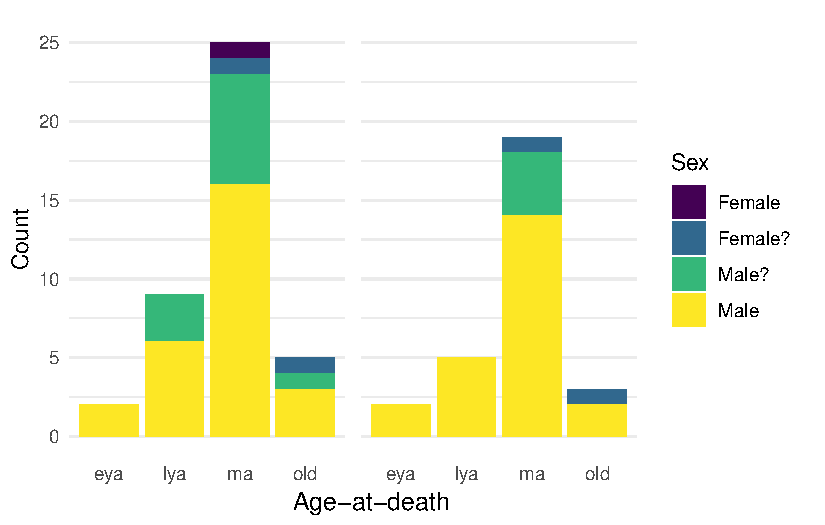
\includegraphics{05-article_files/figure-pdf/fig-sample-demography-1.pdf}

}

\caption{\label{fig-sample-demography}Overview of sample demography.
Left plot is the first batch and right plot is the replication batch
with 29 of the individuals from the first batch. eya = early young adult
(18-24 years); lya = late young adult (25-34 years); ma = middle adult
(35-49 years); old = old adult (50+ years). Male? = probable male;
Female? = probable female.}

\end{figure}

\hypertarget{methods}{%
\section{Methods}\label{methods}}

\hypertarget{skeletal-analysis}{%
\subsection{Skeletal analysis}\label{skeletal-analysis}}

Demographic and pathological analyses were conducted in the Laboratory
for Human Osteoarchaeology at Leiden University. Sex was estimated using
cranial and pelvic morphological traits (Buikstra \& Ubelaker, 1994).
Age-at-death was estimated using dental wear, auricular and pubic
surface appearance, cranial suture closure, and epiphyseal fusion
(Brooks \& Suchey, 1990; Buckberry \& Chamberlain, 2002; Buikstra \&
Ubelaker, 1994; Lovejoy et al., 1985; Meindl \& Lovejoy, 1985), and
divided into the following categories: early young adult (18-24 years),
late young adult (25-34 years), middle adult ( 35-49 years), old adult
(50+ years).

\hypertarget{paleopathology}{%
\subsubsection{Paleopathology}\label{paleopathology}}

Pathological conditions and lesions that occur frequently in the
population were included in the analysis. Data were dichotomised to
presence/absence to allow statistical analysis. Osteoarthritis was
considered present in cases where eburnation was visible on one or more
joint surfaces. Vertebral osteophytosis is identified by marginal
lipping and/or osteophyte formation on the margin of the superior and
inferior surfaces of the vertebral body. Cribra orbitalia was diagnosed
based on the presence of pitting on the superior surface of the orbit.
No distinction was made between active or healing lesions. Degenerative
disc disease, or spondylosis, is identified as a large diffuse
depression of the superior and/or inferior surfaces of the vertebral
body (Rogers, 2000). Schmorl's nodes are identified as any cortical
depressions on the surface of the vertebral body. Data on chronic
maxillary sinusitis from Casna et al. (2021) were included in this study
to assess the relationship between upper respiratory diseases with
environmental factors (i.e.~tobacco smoke, caffeine consumption).
Lesions associated with chronic maxillary sinusitis as defined by
Boocock et al. (1995) were recorded for each individual and classified
as ``pitting'', ``spicule-type bone formation'', ``remodeled spicules'',
or ``white pitted bone''. chronic maxillary sinusitis was scored as
absent when the sinus presented smooth surfaces with little or no
associated pitting.

\hypertarget{dental-pathology}{%
\subsubsection{Dental pathology}\label{dental-pathology}}

Caries ratios were calculated by dividing the number of lesions by the
number of teeth scored, resulting in a single caries ratio per
individual. If the surface where the lesion originated is not visible,
i.e.~if the lesion covered multiple surfaces, this was scored as
``crown''. Calculus indices were calculated according to Greene and
colleagues (2005). Calculus was scored with a four-stage scoring system
(0-3) to score absent, slight, moderate, and heavy calculus deposits
(Brothwell, 1981) on the lingual, buccal (and labial), and interproximal
surfaces of each tooth. Only one score was used for the combined
interproximal surfaces, resulting in three scores per tooth (when
surfaces are intact), and four calculus indices per individual; upper
anterior, upper posterior, lower anterior, lower posterior. Each index
was calculated by dividing the sum of calculus scores for each surface
by the total number of surfaces scored in each quadrant. If a tooth
could not be scored on all three surfaces, the tooth was not included
(T. R. Greene et al., 2005). Periodontitis was scored on a visual
four-stage (0-3) scoring system according to distance from
cemento-enamel junction of each tooth to alveolar bone (Maat \&
Mastwijk, 2005).

\hypertarget{calculus-sampling}{%
\subsection{Calculus sampling}\label{calculus-sampling}}

Where possible, we used material that had already been sampled for a
previous study to prevent unnecessary repeated sampling of individuals.
Calculus from the previous study was sampled in a dedicated ancient DNA
laboratory at the Laboratories of Molecular Anthropology and Microbiome
Research in Norman, Oklahoma, U.S.A, using established ancient DNA
protocols. More details on the methods can be found in the published
articles (Ziesemer et al., 2015, 2018). Of the 41 individuals that were
originally included in our sample, 29 were replicated in a separate
analysis only using calculus from the previous study.\\
New dental calculus samples were taken under sterile conditions in a
positive pressure laminar flow hood in a dedicated dental calculus lab
at Leiden University. The surface of the tooth was lightly brushed with
a sterile, disposable toothbrush to get rid of surface contaminants. A
sterile dental curette was then used to scrape calculus from the tooth
onto weighing paper, which was transferred to 1.5 ml Eppendorf tubes.
All calculus samples were sent to the Department of Forensic Medicine at
Aarhus University for ultra-high-performance liquid
chromatography-tandem mass spectrometry (UHPLC-MS/MS) analysis.

\hypertarget{uhplc-msms}{%
\subsection{UHPLC-MS/MS}\label{uhplc-msms}}

The list of targeted compounds included both naturally occurring
compounds known to have been used in the past, as well as synthetic
modern drugs that did not exist at the time (e.g.~Fentanyl, MDMA,
Amphetamine). These were part of the toxicology screening for the
original method (Sørensen et al., 2021), developed on cadavers. In our
study they serve as an authentication step, as their presence in
archaeological samples could only be the result of contamination.

Briefly, samples of dental calculus were washed three times each with
one mL of methanol (MeOH), to remove surface contaminants. The wash
solutions were collected separately. The solvent was evaporated and the
residues were dissolved in 50 µL 30\% MeOH. The washed calculus was
homogenized in presence of 0.5 M citric acid using a lysing tube with
stainless steel beads. Following one hour of incubation the dissolution
extract was cleaned by weak and strong cation-exchange. After
evaporation of the elution solvent the residue was dissolved in 50 µL
30\% MeOH. The final extracts obtained from washing and dissolution of
the dental calculus were analysed by UHPLC-MS/MS using a reversed-phase
biphenyl column for chromatography. To obtain quantitative results,
isotope dilution was applied. For more details about the method and
validation, see the original study by Sørensen and colleagues (2021).

\hypertarget{statistical-analysis-1}{%
\subsection{Statistical analysis}\label{statistical-analysis-1}}

All compounds and pathological conditions/lesions were converted to a
presence/absence score. Pearson product-moment correlation was applied
to the dichotomised pathological lesions (point-biserial correlation),
compound concentrations, calculus indices, and caries ratios to explore
relationships paired continuous-continuous variables and paired
continuous-binary variables. Compound concentrations were then
dichotomised to presence/absence, and the caries ratio and calculus
index for each individual were converted to an ordinal score from 0 to 4
by using quartiles. Polychoric correlation was applied to the paired
dichotomous variables and dichotomous-ordinal variables.

All statistical analysis was conducted in R version 4.3.0 (2023-04-21),
Already Tomorrow, (R Core Team, 2020). Data wrangling was conducted with
the \textbf{tidyverse} (Hadley Wickham et al., 2019) and visualisations
were created using \textbf{ggplot2} (H. Wickham, 2016). Polychoric
correlations were calculated with the \textbf{psych} package (Revelle,
2022).

\hypertarget{results-1}{%
\section{Results}\label{results-1}}

Multiple compounds were detected in the dental calculus samples.
Compounds detected at a lower concentration than the lower limit of
quantitation (LLOQ) were considered not present. Not all the compounds
detected in the first batch could be replicated in the second batch
(Table~\ref{tbl-compound-detect}). For a full list of targeted
compounds, see Supplementary Material.

\hypertarget{tbl-compound-detect}{}
\begin{longtable}[]{@{}lllr@{}}
\caption{\label{tbl-compound-detect}Target compound including whether it
was detected (TRUE) or not (FALSE) in each batch, as well as the lower
limit of quantitation (LLOQ) in ng. CBD = cannabidiol; CBN = cannabinol;
THC = tetrahydrocannabinol; THCA-A = tetrahydrocannabinolic acid A;
THCVA = tetrahydrocannabivarin acid.}\tabularnewline
\toprule\noalign{}
Compound & Batch 1 & Batch 2 & LLOQ \\
\midrule\noalign{}
\endfirsthead
\toprule\noalign{}
Compound & Batch 1 & Batch 2 & LLOQ \\
\midrule\noalign{}
\endhead
\bottomrule\noalign{}
\endlastfoot
CBD & TRUE & FALSE & 0.050 \\
CBN & TRUE & FALSE & 0.050 \\
Caffeine & TRUE & TRUE & 0.050 \\
Cocaine & TRUE & FALSE & 0.025 \\
Cotinine & TRUE & TRUE & 0.050 \\
Nicotine & TRUE & TRUE & 0.100 \\
Salicylic acid & TRUE & TRUE & 0.500 \\
THC & TRUE & FALSE & 0.100 \\
THCA-A & TRUE & FALSE & 0.025 \\
THCVA & TRUE & FALSE & 0.010 \\
Theophylline & TRUE & TRUE & 0.010 \\
\end{longtable}

The pattern we expect to see in authentic compounds representing
compounds trapped within the dental calculus, is a reduction in the
quantity from wash 1 to wash 3 as potential surface contaminants are
washed off, and then a spike in the final extraction when entrapped
compounds are released and detected.

Most plots show a large increase in extracted mass of a compound between
the calculus wash extracts (wash 1-3) and the dissolved calculus (calc).
Most samples containing theophylline and caffeine had the largest
quantity of the compound extracted from the first wash, then decreasing
in washes 2 and 3. There is an increase between wash 3 and the dissolved
calculus in all samples. The patterns are consistent across batches 1
and 2. Nicotine and cotinine have the same relative quantities in the
samples, i.e., the sample with the highest extracted quantity of
nicotine also had the highest extracted quantity of cotinine
Figure~\ref{fig-auth-plot-batch2}.

\begin{figure}

{\centering 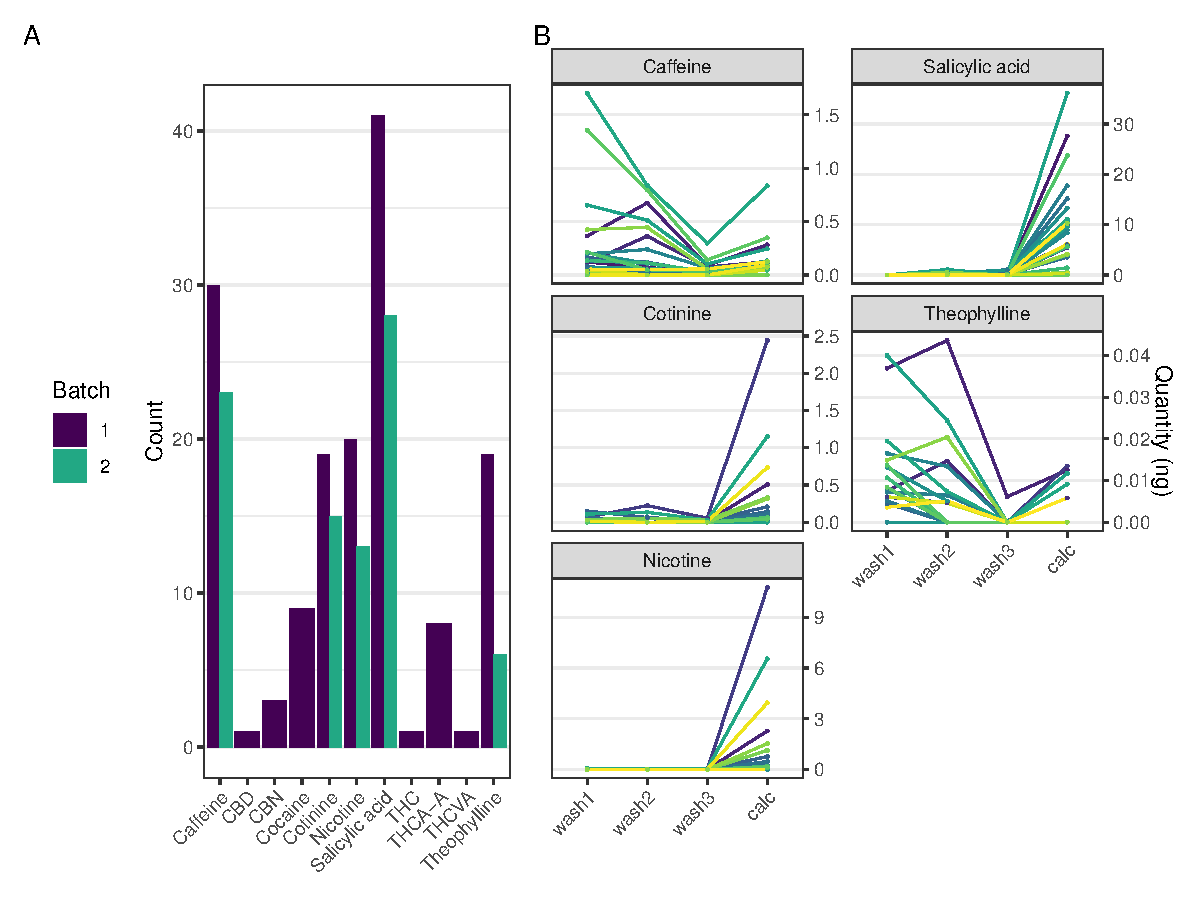
\includegraphics{05-article_files/figure-pdf/fig-auth-plot-batch2-1.pdf}

}

\caption{\label{fig-auth-plot-batch2}(A) Number of samples in which each
compound was detected in the first and second batch. (B) Quantity (ng)
of each compound extracted from each sample in batch 2. The plot
displays the extracted quantity across the three washes and final
calculus extraction (calc). Each coloured line represents a different
calculus sample. CBD = cannabidiol; CBN = cannabinol; THC =
tetrahydrocannabinol; THCA-A = tetrahydrocannabinolic acid A; THCVA =
tetrahydrocannabivarin acid.}

\end{figure}

To see if preservation of the skeletal remains had any effect on the
detection of compounds, we compare extracted quantities of compounds to
the various levels of skeletal preservation. Our results from batch 2
suggest that detection of a compound may be linked to the preservation
of the skeleton, with better preservation leading to increased
extraction quantity (Figure~\ref{fig-detection-preservation}A). We also
find a weak positive correlation between the weight of the calculus
sample and the quantity of compound extracted from the calculus
(Figure~\ref{fig-detection-preservation}B).

\begin{figure}

{\centering 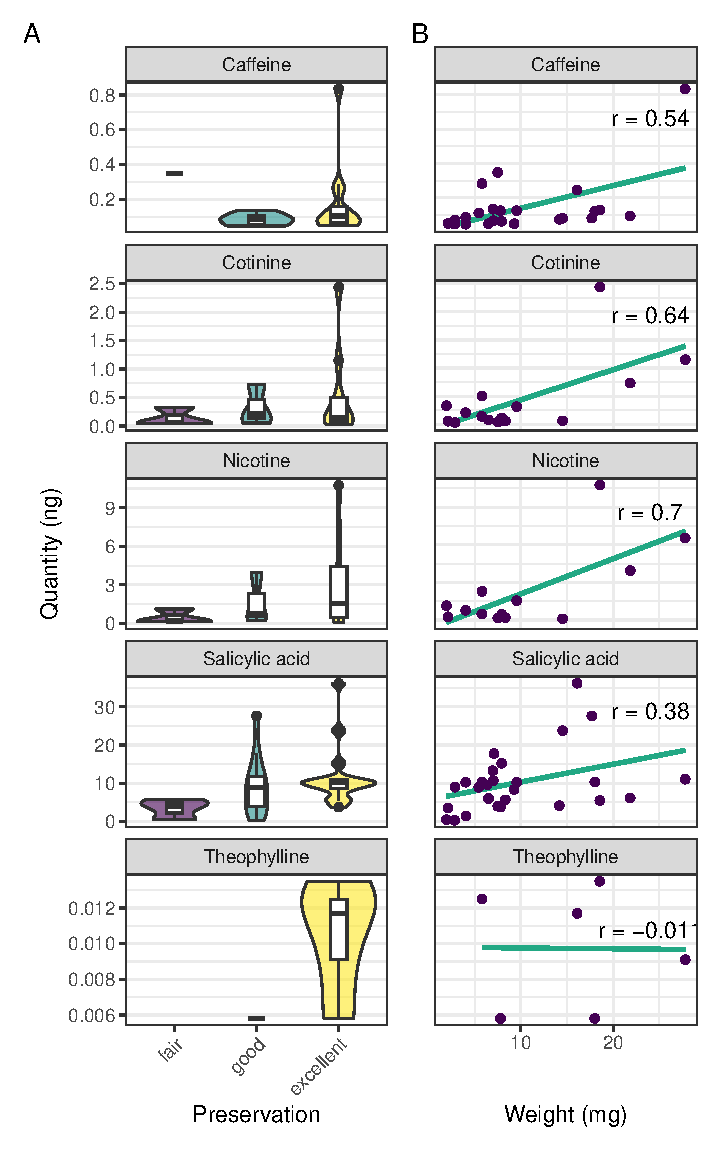
\includegraphics{05-article_files/figure-pdf/fig-detection-preservation-1.pdf}

}

\caption{\label{fig-detection-preservation}(A) Violin plot with overlaid
box plots depicting the distribution of extracted quantities of each
compound from batch 2 separated by state of preservation of the
skeleton. (B) Extracted quantity (ng) of compound plotted against
weights of the calculus samples from batch 2.}

\end{figure}

The presence of pipe notch(es) in an individual and concurrent detection
of nicotine and/or cotinine is used as a crude indicator of the accuracy
of the method. Only males were used in accuracy calculations, as pipe
notches are ubiquitous in males, but not in females. In batch 2, the
method was able to detect some form of tobacco in 14 of 25 individuals
with a pipe notch (56.0\%). When also considering correct the absence of
a tobacco alkaloid together with the absence of a pipe notch, the
accuracy of the method is 59.3\%. Accuracy in the old adult age category
is 100.0\%, but with only 2 individuals.

One individual---an old adult, probable female---was positive for both
nicotine and cotinine, and had no signs of a pipe notch.

\hypertarget{correlations-between-detected-alkaloids-and-diseases}{%
\subsection{Correlations between detected alkaloids and
diseases}\label{correlations-between-detected-alkaloids-and-diseases}}

For further statistical analyses, only the UHPLC-MS/MS results from
batch 2 were used, as batch 1 had multiple compounds that were not
detected in batch 2 and may have been contaminated.

\hypertarget{tbl-pearson}{}
\begin{longtable}[]{@{}
  >{\raggedright\arraybackslash}p{(\columnwidth - 16\tabcolsep) * \real{0.1566}}
  >{\raggedright\arraybackslash}p{(\columnwidth - 16\tabcolsep) * \real{0.0843}}
  >{\raggedright\arraybackslash}p{(\columnwidth - 16\tabcolsep) * \real{0.1084}}
  >{\raggedright\arraybackslash}p{(\columnwidth - 16\tabcolsep) * \real{0.0843}}
  >{\raggedright\arraybackslash}p{(\columnwidth - 16\tabcolsep) * \real{0.1084}}
  >{\raggedright\arraybackslash}p{(\columnwidth - 16\tabcolsep) * \real{0.0843}}
  >{\raggedright\arraybackslash}p{(\columnwidth - 16\tabcolsep) * \real{0.1566}}
  >{\raggedright\arraybackslash}p{(\columnwidth - 16\tabcolsep) * \real{0.1084}}
  >{\raggedright\arraybackslash}p{(\columnwidth - 16\tabcolsep) * \real{0.1084}}@{}}
\caption{\label{tbl-pearson}Pearson correlation (\emph{r}) on
dichotomous skeletal lesions and compound concentrations (ng/mg) from
the second batch. Correlations between pairs of dichotomous variables
are removed due to incompatibility with a Pearson correlation. OA =
osteoarthritis; VOP = vertebral osteophytosis; SN = Schmorl's nodes; DDD
= degenerative disc disease; CO = cribra orbitalia; CMS = chronic
maxillary sinusitis; SA = salicylic acid; PN = pipe
notches.}\tabularnewline
\toprule\noalign{}
\begin{minipage}[b]{\linewidth}\raggedright
\end{minipage} & \begin{minipage}[b]{\linewidth}\raggedright
Caries
\end{minipage} & \begin{minipage}[b]{\linewidth}\raggedright
Nicotine
\end{minipage} & \begin{minipage}[b]{\linewidth}\raggedright
SA
\end{minipage} & \begin{minipage}[b]{\linewidth}\raggedright
Calculus
\end{minipage} & \begin{minipage}[b]{\linewidth}\raggedright
PN
\end{minipage} & \begin{minipage}[b]{\linewidth}\raggedright
Theophylline
\end{minipage} & \begin{minipage}[b]{\linewidth}\raggedright
Caffeine
\end{minipage} & \begin{minipage}[b]{\linewidth}\raggedright
Cotinine
\end{minipage} \\
\midrule\noalign{}
\endfirsthead
\toprule\noalign{}
\begin{minipage}[b]{\linewidth}\raggedright
\end{minipage} & \begin{minipage}[b]{\linewidth}\raggedright
Caries
\end{minipage} & \begin{minipage}[b]{\linewidth}\raggedright
Nicotine
\end{minipage} & \begin{minipage}[b]{\linewidth}\raggedright
SA
\end{minipage} & \begin{minipage}[b]{\linewidth}\raggedright
Calculus
\end{minipage} & \begin{minipage}[b]{\linewidth}\raggedright
PN
\end{minipage} & \begin{minipage}[b]{\linewidth}\raggedright
Theophylline
\end{minipage} & \begin{minipage}[b]{\linewidth}\raggedright
Caffeine
\end{minipage} & \begin{minipage}[b]{\linewidth}\raggedright
Cotinine
\end{minipage} \\
\midrule\noalign{}
\endhead
\bottomrule\noalign{}
\endlastfoot
OA & -0.19 & -0.074 & 0.21 & 0.07 & 0.14 & 0.28 & 0.00098 & -0.067 \\
VOP & -0.061 & -0.16 & 0.34 & 0.061 & 0.25 & -0.06 & 0.013 & -0.13 \\
SN & -0.22 & 0.16 & 0.095 & 0.089 & 0.17 & 0.24 & 0.16 & 0.093 \\
DDD & 0.032 & 0.0037 & 0.19 & -0.39 & -0.077 & 0.31 & 0.06 & -0.0086 \\
CO & 0.14 & -0.051 & 0.2 & 0.14 & -0.2 & -0.11 & 0.19 & -0.065 \\
CMS & -0.18 & 0.28 & 0.0017 & -0.27 & 0.032 & 0.19 & 0.36 & 0.22 \\
Caries & & -0.13 & -0.27 & -0.19 & -0.037 & -0.16 & 0.079 & -0.16 \\
Nicotine & & & -0.21 & 0.01 & -0.014 & 0.43 & 0.14 & 0.98 \\
SA & & & & 0.14 & 0.37 & 0.038 & 0.17 & -0.17 \\
Calculus & & & & & 0.13 & -0.15 & -0.13 & 0.031 \\
PN & & & & & & -0.16 & 0.18 & -0.0068 \\
Theophylline & & & & & & & 0.51 & 0.36 \\
Caffeine & & & & & & & & 0.078 \\
\end{longtable}

Point-biserial correlation was conducted on paired continuous and
dichotomous variables, to see if any relationships exist between
extracted concentrations and other variables. The strongest
point-biserial (Pearson) correlation correlations were a near-perfect
positive correlation between cotinine and nicotine (0.982), and moderate
correlations between theophylline and nicotine (0.432), caffeine and
theophylline (0.507) (Table~\ref{tbl-pearson}).

Polychoric correlation was conducted on the dichotomised compounds and
pathological conditions, as well as the discretised dental diseases.
Salicylic acid was removed due to its ubiquitous presence in the sample,
and is likely to cause spurious correlations. Strong correlations were
found between cotinine and nicotine (0.851). Moderate correlations were
found between OA and DDD (0.484), VOP and periodontitis (0.491), SN and
cotinine (0.558), DDD and calculus (-0.421), CMS and caffeine (0.528),
caries and periodontitis (0.486), caries and theophylline (-0.491),
periodontitis and caries (0.486), periodontitis and caffeine (0.515),
nicotine and CMS (0.496), calculus and caries (0.502), age-at-death and
theophylline (-0.447), theophylline and age-at-death (-0.447), caffeine
and periodontitis (0.515), cotinine and CMS (0.425). Remaining
correlations were weak or absent (Figure~\ref{fig-polycorr}).
Correlations with age will be depressed because age was largely
controlled for in the sample selection.

\begin{figure}

{\centering 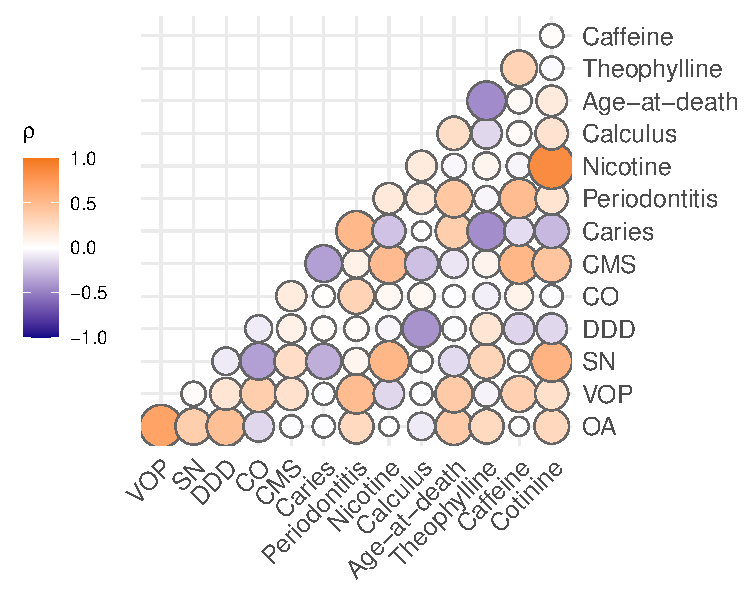
\includegraphics{05-article_files/figure-pdf/fig-polycorr-1.pdf}

}

\caption{\label{fig-polycorr}Plot of the polychoric correlations
(\emph{rho}). Larger circles and increased opacity indicates a stronger
correlation coefficient. OA = osteoarthritis; VOP = vertebral
osteophytosis; SN = Schmorl's nodes; DDD = degenerative disc disease; CO
= cribra orbitalia; CMS = chronic maxillary sinusitis; SA = salicylic
acid.}

\end{figure}

\hypertarget{discussion-1}{%
\section{Discussion}\label{discussion-1}}

In this study we were able to extract and identify multiple alkaloids
and salicylic acid from the dental calculus of individuals from
Middenbeemster, a 19th century Dutch archaeological site. We applied
ultra-high-performance liquid chromatography-tandem mass spectrometry
(UHPLC-MS/MS), a method that was validated by co-occurrence of drugs and
metabolites in dental calculus and blood (Sørensen et al., 2021). Here
we have shown that the method can also be successfully applied to
archaeological dental calculus. We extend findings from previous studies
on alkaloids in archaeological samples by extracting multiple different
alkaloids from dental calculus, including nicotine, cotinine, caffeine,
theophylline, and salicylic acid in multiple individuals. The detection
of these compounds was solidified in a replication analysis on different
samples from the same individuals. Cocaine and multiple cannabinoids
were also detected during the first analysis, but were not replicated.
We discuss the implications of these findings in light of historical and
archaeological evidence for the consumption of these drugs.

Nicotine and its principal/main metabolite, cotinine, were strongly
positively correlated, both in concentration and presence/absence in
individuals (Table~\ref{tbl-pearson} and Figure~\ref{fig-polycorr}). The
detection of nicotine and cotinine is not surprising, as pipe-smoking in
the Beemsterpolder is well-documented in the literature (Aten et al.,
2012; Bouman, 2017), and visible on the skeletal remains as pipe notches
(Lemmers et al., 2013). There is also documented medicinal use of
nicotine in the Beemsterpolder, where a tobacco-smoke enema was used for
headaches, respiratory problems, colds, and drowsiness from around 1780
to 1830 (Aten et al., 2012). In our sample, we also detected nicotine
and cotinine (replicated) in an old adult, probable female individual.
In this particular case it is unlikely that the compounds entered the
dental calculus through pipe-smoking, as the individual had no visible
pipe notches; more likely the tobacco entered through an alternate mode
of consumption, secondhand smoke, or the aforementioned tobacco-smoke
enema.

Theophylline and caffeine were positively correlated in our samples,
though to a lesser extent than nicotine and cotinine, so we are unable
to determine if they originated from the same source
(Table~\ref{tbl-pearson} and Figure~\ref{fig-polycorr}). Caffeine and
theophylline have very similar chemical structures, so we expect they
would experience similar rates of incorporation and degradation,
allowing us to interpret the ratio and correlations between the
compounds. Caffeine is present in coffee, tea, and cocoa beans, with
concentrations slightly higher in coffee (Bispo et al., 2002; Chin et
al., 2008; Srdjenovic et al., 2008; Stavric et al., 1988). Theophylline
is present in both coffee beans and tea leaves, but in negligible
quantities (Stavric et al., 1988). It is also a primary metabolite of
caffeine produced by the liver. Given the low correlation, there are
likely multiple sources of caffeine and theophylline in the population,
with tea and coffee being the most obvious.\\
Tea consumption had become widespread in the Netherlands by 1820,
reaching all parts of society (Nierstrasz, 2015, p. 91). Historically,
we also know that both tea and coffee were consumed in the
Beemsterpolder during the 19th century. `Theegasten' (teatime) was a
special occasion occurring from 15.00-20.00 hours, where tea was served
along with the evening bread (Schuijtemaker, 2011). Many households also
owned at least one coffee pot and tea pot (Bouman, 2017). Distinguishing
between tea, coffee, and chocolate may be possible by also including
theobromine and comparing ratios of the compounds, as theobromine is
present in higher quantities in chocolate compared to caffeine and
theophylline (Alañón et al., 2016; Bispo et al., 2002; Stavric et al.,
1988). However, In addition to oral factors affecting alkaloid uptake in
dental calculus, there is some indication that theobromine does not
preserve well in the archaeological record (Velsko, Overmyer, et al.,
2017), and frequent consumption of all three items would be difficult to
parse.

Salicylic acid was found in all but one individual in our sample. It can
be extracted from the bark of willow trees, \emph{Salix alba}, and has
long been used for its pain-relieving properties (Bruinsma, 1872, p.
119). It is also present in many plant-based foods (Duthie \& Wood,
2011; Malakar et al., 2017), including potatoes, which were a staple of
the Beemsterpolder diet (Aten et al., 2012). The extracted quantity from
our samples decreased over the three washes, followed by a sharp
increase in the final calculus extraction, which is what we would expect
to see if the salicylic acid was incorporated during life
Figure~\ref{fig-auth-plot-batch2}. However, it has been shown that
salicilyc acid is a very mobile organic acid and the ubiquitous presence
may be due to environmental contamination, which would also explain the
high quantity in the washes (Badri \& Vivanco, 2009; H. Chen et al.,
2001). Given the multiple plausible sources of this residue, it will be
necessary to explore the extent to which salicylic acid can leach into
the dental calculus from the soil, and what the rate of degradation is
for salicylic acid when trapped in dental calculus.

Cannabinoids---specifically THC, THCA-A, THCVA, CBD, CBN---were found in
the first batch, but none were replicated in the second batch. Medicinal
use of cannabinoids has been well-established in Europe since
Medieval-times, and it was also grown in the Netherlands (Bruinsma,
1872). Administration was most common in the form of concoctions
containing various portions of the cannabis plant for ingestion; not
until the late 19th century did it become recommended to smoke it for
more immediate effects (Clarke, 2013). A Dutch medicinal use of hemp
involved an emulsion prepared from the seeds of the plants to treat pain
and various stomach ailments. Another preparation involving the roots of
the plants was used for inflammation, gout, and joint pains (Clarke,
2013). The ability to detect cannabinoids in calculus may be limited by
their reduced ability to diffuse from serum to salivary glands due to an
affinity for protein-binding, (Cone \& Huestis, 2007), meaning detection
would rely on oral consumption. Even then, the overall instability of
some cannabinoids could also affect detection (Lindholst, 2010; Sørensen
\& Hasselstrøm, 2018). However, given the lack of replication, we cannot
with security confirm that cannabis was used by the Beemster population.

Despite many of our sampled individuals having lived during the height
of the opium era in the Netherlands (Macht, 1915), none of the targeted
opioids (morphine, codeine, thebaine, papaverine, norcodeine, noscapine)
were detected. The absence of opioids could be a result of the people
ascribing more to the ``traditional'' rather than ``scientific''
medicine, although laudanum and another opium containing concoction was
part of the ``traditional'' medicine in the Netherlands (Leuw \&
Marshall, 1994), including Middenbeemster (Aten et al., 2012). It was
also generally considered a drug of the upper class (Scheltema, 1907),
and may have been more common in urban centers. The absence could also
be attributed to postmortem degradation. It has been shown that, while
abundant in opium, morphine degrades rapidly, while thebaine and
papaverine are more resistant to various ageing processes (Chovanec et
al., 2012). The latter were also absent from our samples.

The only strictly modern compound (at least in a European context)
detected in the sample was cocaine, which was detected in the first
batch of samples. Our sample is derived from an early--mid 19th century
population, and cocaine was isolated in 1860 by Albert Niemann, and
entered popular medical practice in 1884. Coca arrived in Europe as
early as 1771, but as botanical specimens rather than for consumption,
and there were also issues importing enough viable specimens of coca for
cocaine extraction (Abduca, 2019, p. 108; Mortimer, 1901, p. 179). We
considered it possible that it would be present in a sample with most
individuals originating from the early- to mid-19th century. If
corroborated, this would have been the first case of
coca-leaf-consumption in Europe. In our replication batch, we included
all of the individuals who had been cocaine-positive in the first batch.
We were unable to replicate any of the cocaine results, and we were
unable to detect the principal metabolite, benzoylecgonine, in either
batch. We suspect that the original detection of cocaine was a result of
lab contamination during analysis.

We explored the relationship between detected compounds and various
skeletal indicators, such as pathological and dental lesions,
preservation, and pipe notches. We found some evidence to suggest that
preservation of the skeleton influences the recovery of compounds from
the dental calculus, with well-preserved skeletons potentially serving
as a better target for sampling.\\
We found a positive correlation between CMS and nicotine, which may be
indicative of the impact tobacco smoking had on the respiratory health
of the Beemster inhabitants. Tobacco smoke may play a significant role
in diseases of the upper respiratory tract, including chronic maxillary
sinusities (Reh et al., 2012). Although the mechanisms by which smoking
increases the risk of infections is not fully understood, solid evidence
has been presented linking tobacco smoke to increased mucosal
permeability and impairment of mucociliary clearance (Arcavi \&
Benowitz, 2004). Such changes, together with an altered immunologic
response, are thought to predispose to the development of chronic
maxillary sinusitis (Slavin et al., 2005).\\
We also observed a moderate positive correlation between chronic
maxillary sinusitis and caffeine which contradicts previous research
linking chronic coffee consumption with a positive effect on the
respiratory system, suggesting a preventive association between caffeine
intake and pneumonia (e.g. Alfaro et al., 2018; Kondo et al., 2021).
However, while the lower respiratory tract seems to benefit from chronic
coffee consumption, it is possible that elevated caffeine intake impacts
mucosal moisture due to its dehydrating effect (Maughan \& Griffin,
2003), thereby exposing individuals to greater risk of sinus infection.

The detection of nicotine in dental calculus has previously been
presented by Eerkens and colleagues (2018) in two individuals from
pre-contact California. They also targeted caffeine, cotinine, and
theophylline in their samples, but were unable to detect any of them. It
remains to be seen whether this is due to differences in methods used,
or due to our samples being more recent. They also suggest that the
choice of tooth for sampling may impact the detection of certain
compounds, as the incorporation in dental calculus may depend on the
mode of consumption. Tobacco smokers may have more nicotine present in
calculus on incisors, whereas tobacco chewers may have more on molars
(Eerkens et al., 2018). However, sampling may not be limited to mode of
consumption. The presence of cotinine suggests that the excretion of a
compound after being metabolised in the body is also a source of
deposition, and that deposition of alkaloids in dental calculus can
occur both on the way into the body, i.e.~during consumption, and on the
way out, i.e.~disposal of waste products via saliva secretion into the
mouth. Especially mucin-rich saliva from the sublingual and
submandibular glands preferentially binds toxins (Michael W. J. Dodds et
al., 2005), and since these glands are located closest to the lower
incisors, they may be the most effective target for these studies. This
has yet to be systematically tested in archaeological dental calculus.
Because we homogenised samples from multiple teeth of an individual, we
were unable to test the effect of oral biogeography. It is also possible
that resident microflora within biofilms contribute to alkaloid
breakdown and that the presence of caffeine and nicotine metabolites
following direct ingestion can be explained by this pathway. However,
the literature on biofilm biodegradation of alkaloids is limited, and
\emph{in vitro} studies have only found minimal contributions by certain
oral bacteria in isolation (Cogo et al., 2008; Sun et al., 2016); it is
possible that a larger role is played by oral bacteria within larger,
more metabolically active communities, e.g.~biofilms (Takahashi, 2015).

Because we targeted individuals with moderate-to-large calculus
deposits, it is likely a biased sample. The presence of calculus may
increase the risk of premature death (Yaussy \& DeWitte, 2019), and
periodontal disease (which may or may not be associated with dental
calculus build-up) is a risk-factor for respiratory diseases, if
periodontal and respiratory pathogens enter the bloodstream (Azarpazhooh
\& Leake, 2006; Scannapieco, 1999; Scannapieco \& Ho, 2001). In our
sample, the percentage of chronic maxillary sinusitis (37.0\%) is lower
than in another (more representative) male sample (44.1\%) (Casna et
al., 2021), and the caries percentage is similarly lower in our sample
(12.7\%) than a more representative sample (22.9\%) (Lemmers et al.,
2013).\\
We used the presence/absence of a pipe notch and concurrent detection of
tobacco as a crude estimate of the accuracy of the method, which we
found to be around 59.3\%. This is a very rough estimate, as the
presence of a pipe notch is likely not a perfect indicator of whether or
not someone consumed tobacco. Dental calculus is also more transient
than for example bone, as it can be mechanically removed, intentionally
or unintentionally, during life, eliminating all trace of the alkaloids
consumed prior to its removal.\\
Quantitation of the detected compounds may have limited value in
archaeological samples due to degradation, and will greatly affect our
correlations related to concentration. Following burial, compound
stability over time will play a large role, as will microbial
degradation of compounds by bacteria and fungi in soil (Liu et al.,
2015), as well as the soil environment, such as temperature, pH, and
oxygen availability (Lindholst, 2010; Mackie et al., 2017).\\
The detected quantity of a compound will also depend on the quantity in
dental calculus during life, which is largely controlled by quantity of
consumption, how often the calculus was disrupted/removed, metabolic
breakdown of the compound, and inter- and intra-individual factors
related to stages of biofilm formation, maturation, and mineralisation
(Lustmann et al., 1976; Velsko et al., 2019; Zijnge et al., 2010). In
short, this means it is not really possible to detect the absence of a
compound. The absence of a compound is not evidence of absence of
consumption. This complicates the interpretation of our results. We have
attempted to minimise errors occurring due to this limitation by
including a relatively large sample of individuals and replicating our
analysis. Although given the relatively low detection rate seen in
tobacco, this remains a major limitation, and will likely be compounded
by increasing antiquity of the samples.

Future studies should explore how sampling from various types of teeth
and their position in the mouth affects the probability of a compound
becoming entrapped in dental calculus. This may also be related to
properties within the oral cavity, as well as chemical properties of the
compounds, which facilitate or reduce the incorporation-potential, and
which incorporation pathways are more likely for a given compound.\\
We only targeted drugs that were included in the forensic toxicological
screenings, and therefore only covered a limited number of the potential
compounds that could be of interest for exploring past diets and
medicinal treatments. The list of targeted compounds can be expanded as
we discover more potential targets based on which specific
compounds/metabolites are more likely to be incorporated and preserved
in dental calculus.\\
There is an increasing interest in using oral fluid as a means of
detecting alkaloids in living individuals due to the non-invasive nature
of the testing compared to blood and urine sampling (Cone, 1993; Valen
et al., 2017). These \emph{in vivo} studies are a valuable source of
method validation and can help determine the feasibility of detecting
certain alkaloids in oral fluid and, subsequently, dental calculus.
Archaeologists, though, will likely be responsible for exploring dental
calculus specific incorporation and retention of alkaloids, as well as
their long-term preservation in the burial environment.

While a major limitation is the uncertainty surrounding whether or not a
compound is actually absent, the power of the method lies in the ability
to detect dietary and other compounds that were incorporated via
multiple consumption pathways that are not detected by other methods.
Taking tobacco consumption as an example; while pipe notches are a
useful way to identify tobacco consumption, pipe smoking was not the
only mode of tobacco consumption, with others including chewing,
drinking, cigars, and snuff (Goodman, 1994, p. 67). Pipe-smoking was
mainly practised by males (Eerkens et al., 2018; Lemmers et al., 2013),
so methods like the one presented here are suitable for exploring
tobacco consumption in an entire society, rather than a trivial subset
of past populations. Combined with other methods, it can also give us a
more complete picture of dietary patterns and medicinal/recreational
plant-use in the past by capturing multiple possible incorporation
pathways of dietary (and other) compounds.

\hypertarget{conclusion-1}{%
\section{Conclusion}\label{conclusion-1}}

This preliminary study outlines the benefits of using calculus to target
a variety of compounds that could have been consumed as medicine or
diet. This method allows us to directly address specific individuals,
which can be especially useful in individuals that are not always
well-documented in historic documentation, such as rural communities,
children and women. We also show that there are many limitations that
will need to be addressed going forward with this type of analysis, and
stress the need for more systematic research on the consumption of
alkaloid-containing items and their subsequent concentration and
preservation in dental calculus, in addition to how mode of consumption
may affect concentrations on different parts of the dentition. Another
limitation of dental calculus as a medium is the inter- and
intra-individual variability of its formation and the many factors that
can influence incorporation and retention of molecules and particles;
however, in the absence of hair and serum (quite uncommon in
archaeology), dental calculus represents an impressive long-term
reservoir of information regarding the consumption of various alkaloids,
whether dietary, medicinal, recreational, or otherwise.

\hypertarget{references-1}{%
\section*{References}\label{references-1}}
\addcontentsline{toc}{section}{References}

\markright{References}

\bookmarksetup{startatroot}

\hypertarget{chap-discussion}{%
\chapter{Discussion}\label{chap-discussion}}

Archaeological researchers are presented with a unique challenge.
Because time eventually degrades everything, the archaeological record
will always be incomplete. Barring the invention of time travel---and
depending where you land on the discussion of travelling back to a time
before time travel is invented---we are limited in our ability to fill
in these gaps in our knowledge.

Consider it a puzzle that needs to be put back together, only some
pieces are permanently missing, and other pieces are broken. Researchers
will attempt to fill in the gaps (complete the puzzle) with
interpretations based on observations\ldots{} To further complicate
things, the methods we use may be biased causing additional pieces of
the puzzle to go missing. Some things cannot be validated on
archaeological remains, since we are missing key information about
conditions in the past. Take for example dental calculus. Archaeologists
often use it to reconstruct the diet of past populations\ldots{}

As shown in \protect\hyperlink{fig-plot-and-wordclouds}{Chapter 1},
dental calculus has become a very popular substance within
archaeological research, to the point where it has surpassed its use in
dental research, at least in terms of articles where it is the main
topic of focus. While the use of oral biofilm models in dental research
is well-established, even long-term calcifying models to produce dental
calculus, they never made it into archaeological research. At least not
to the extent that they were published.

There is also a lack of fundamental research and experimentation being
conducted within the fields that make use of archaeological dental
calculus. There are of course exceptions (Leonard et al., 2015; R. C.
Power et al., 2015; Robert C. Power et al., 2021; Soto et al., 2019),
but these have not addressed the full extent of dental calculus
limitations (nor should they).

the model outlined in this dissertation is in no way the ultimate
solution to save us from the limitations of the archaeological record,
but may provide a small step towards understanding them a little better,
and hopefully promote further exploration through fundamental research.

In this dissertation, I have mainly focused on the development,
validation, and application of an oral biofilm model and its potential
for informing archaeological research. I have shown that it was possible
to develop a protocol for an oral biofilm model with a relatively simple
setup, and use it to grow artificial dental calculus. I also showed that
it can serve as a reasonable proxy to natural dental calculus
(\protect\hyperlink{byoc-valid}{Chapter 3}).

The two articles that make up chapters 3 and 4 show some of the possible
contributions an oral biofilm model can make to the field of
archaeological research.

I demonstrated how the oral biofilm model can answer questions and
identify hidden biases related to using dental calculus for paleodietary
reconstructions, specifically addressing the identification and
quantification of starch granules. The results from this study showed
that what goes in, doesn't necessarily come out. And the loss of
information is not evenly distributed across the different types of
starches, depending on size and morphology
{[}\protect\hyperlink{byoc-starch}{Chapter 4}; Bartholdy \& Henry
(2022){]}.

In \protect\hyperlink{mb11CalculusPilot}{Chapter 5} I present a study
that goes beyond the model and looks at archaeological dental calculus.
This is, after all, a dissertation in archaeology. We analysed dental
calculus samples from a rural Dutch archaeological site in
Middenbeemster, using ultra high performance liquid chromatography
tandem mass spectrometry (UHPLC-ESI-MS/MS). This allowed us to identify
a number of residues from plants that may have been consumed for
nutrition, medicine, recreation, or all of the above.

\hypertarget{the-dental-calculus-model}{%
\section{The dental calculus model}\label{the-dental-calculus-model}}

The goal of developing a dental calculus model was to explore core
aspects of how we use dental calculus in paleodietary research, with a
relatively simple setup that is accessible to most labs in
archaeological science. The idea is to take a step back and really
scrutinise our current methods for interpreting diet from dental
calculus. What the field has accomplished so far is undeniably
impressive, but there are many things we still don't understand. Some of
the things we don't understand are on a very basic level, such as how
plant microremains become trapped inside calculus, how much of what we
consume ends up inside calculus, and whether our current methods are
able to accurately extract that information.

The model we chose was a simple model using a shaking incubator and a 24
deepwell plate with the plastic lids as a substratum. The artificial
saliva we used was based on the basal modified medium used by Sissons
and colleagues (1991, 1994; 1997) to grow dental calculus. We also made
use of their calcifying solution, calcium phosphate monofluorophosphate
urea (CPMU). To make sure the calculus we were growing in the lab was a
good model for calculus grown naturally, we sequenced the DNA of our
model calculus and compared it to various sites inside the human mouth,
including dental plaque and calculus. The bacterial composition of our
model calculus samples had a strong oral signature, but was distinct
from other natural oral samples, including dental plaque and calculus.
The main difference between natural samples and model calculus was that
the natural samples were more heterogenous in composition. They had a
larger number and variety of microbes compared to the model calculus.
This was also reflected in the aerotolerance of dominant microbes in
model calculus, which were largely anaerobes, while natural samples had
more aerobes and facultative anaerobes. The natural samples also had a
more diverese representation of bacteria from all stages of biofilm
development, including early- middle-, and late-colonisers, while model
calculus samples were predominantly late-colonisers
{[}\protect\hyperlink{byoc-valid}{Chapter 3}; Bartholdy, Velsko, et al.
(2023){]}.

Our metagenomics results were similar to a comparable \emph{in vitro}
biofilm model. In the study, the authors also used a 24-well plate with
pooled saliva as inoculate. The growth medium was similar but also
contained a sheep's-blood serum, and the samples were only grown for 24
hours (Edlund et al., 2018). As with our model, the comparison with
natural oral samples showed a lower overall richness and diversity, and
a distinct microbial profile {[}\protect\hyperlink{byoc-valid}{Chapter
3}; Bartholdy, Velsko, et al. (2023){]}. Given that our results are
similar to a short-term biofilm model, we may be replacing the medium
too frequently (every three days), and not allowing communities to
establish more complex metabolic pathways present in mature biofilms.

We also used Fourier Transform Infrared (FTIR) spectroscopy to \ldots{}
the mineral content of our model, and also compare that to natural
dental calculus, both modern and archaeological. Our analysis using FTIR
spectroscopy showed that our biofilm model, after 25 days of growth,
produced a substance that is chemically very similar to both modern and
archaeological calculus. The crystallinity of the model calculus also
matched the archaeological sample we used as a comparison, though with a
slightly less ordered structure. This may be related to the age
differences in model calculus compared to archaeological calculus. Not
only did the archaeological calculus spend a few hundred years maturing
in the ground, allowing crystals to expand into the gaps created by
degraded organic matter (Weiner, 2010), but given the known lack of oral
hygiene practices in the past, the calculus was likely older than 25
days before being buried. We also only analysed a single archaeological
sample, so we don't know how representative this sample is of
archaeological samples in general. Perhaps this was a particularly
under- or over-mineralised sample. It would be more appropriate to
compare to the modern reference samples, since we are actually trying to
recreate something that mimics natural modern calculus, not something
that has been buried for hundreds of years or more. Unfortunately we
didn't have access to new modern samples and couldn't produce modern
calculus grind curves for this analysis.

It is interesting that the mineral composition was so similar to natural
calculus given the unique microbial profile. It suggests that the
mineralisation occurs if conditions are favourable, regardless of the
microbial profile. Even in the absence of known mineraliser,
\emph{Corynebacterium matruchotii}. Since FTIR only addresses the
overall mineral composition, we will need to further investigate whether
there are any other structural/chemical differences between our model
and natural calculus that may be caused by microbial profiles.

Further refining the protocol can be a solution to this. Using serum in
the medium to establish thicker and more stable biofilms, allowing
slow-growing organisms to become more established (Ammann et al., 2012).
Filter-sterilising the heat-sensitive solutions that are not autoclaved,
such as CPMU and starch solutions, may prevent environmental
contamination from entering the biofilm during the setup, such as
members of the \emph{Enterococcus} genus. While these are commonly
present in oral samples,

Changes to the model setup will have to be re-validated, as the
concentrations of nutrients, let alone the type of nutrients, will
impact the community composition of the biofilms (Edlund et al., 2013).

Further validation\ldots{} physiological response to changing
conditions. For example, after carbohydrates have been consumed, there
is a dip in the pH within the oral cavity as the carbohydrates are
consumed by bacteria, which release acidic by-products. This occurs
within the first few hours of consuming carbohydrates, after which the
saliva will work to balance the pH back to pre-carbohydrate levels, also
known as the `Stephan curve' (Stephan \& Hemmens, 1947). By acting as a
buffer and restoring the oral pH-level, saliva can help prevent high
levels of acid from demineralising the tooth surface and causing caries.
Since our model is fed both with sucrose and starch, it is important to
know that the pH levels don't permanently drop to levels that are
unfavourable to mineral supersaturation and plaque mineralisation.

After establishing that our model dental calculus mimics, at least to
some extent, the real deal, we assessed what biases may occur in starch
incorporation. Put simply, we added a known amount of starch
granules---well, to the extent we could estimate the large quantities in
our starch solutions without counting every single granule---to our
biofilm over the course of the 25-day experiment. Then we dissolved the
calculus and counted the number of starches that that were inside. Those
who are familiar with previous dietary research on archaeological dental
calculus will probably not be surprised that the number of starches we
extracted was nowhere near the amount we put in. More interestingly,
though, the size of the starch granules influenced the outcome; fewer
large starches were extracted than what was put in. This could be
related to how starch granules are trapped in biofilms in the first
place, where size and/or surface morphology of the starch granules can
influence the likelihood of being retained in the biofilm.

It is a mistake to think you can solve any major problems just with
potatoes (Adams, 2002a), so we also included wheat starches in the model
to cover a wider range of granule shapes and sizes.

\hypertarget{disc-model-limitations}{%
\subsection{Model limitations}\label{disc-model-limitations}}

So far I have covered what our biofilm model can do. It is equally
important to talk about what our model can't do.

While we have a high degree of control and reproducibility, especially
when compared to \emph{in vivo} models, there are certain conditions we
cannot regulate. This includes environmental conditions such as
CO\textsubscript{2} and oxygen availability, which rely on the
conditions in the lab where the experiments take place. We also lack the
ability to control salivary flow rates and circadian rhythms, both of
which can influence the growth of plaque. It also includes the final
microbial composition of the calculus. We use whole saliva as the
inoculate, so the microbial profiles of the biofilms may change
depending on the saliva donors and even on the time of day that the
saliva was collected.

The very isolated and controlled model setup also deviates from the
conditions in someones mouth. Many of the natural predators of the
biofilm are not present. Plaque is constantly at risk of dislodgement by
the tongue, salivary flow, and toothbrushing and other oral hygiene.

As shown in a previous study, calculus and plaque have distinct
microbial profiles (Velsko et al., 2019), so the applicability of
short-term models to explore archaeological questions on dental calculus
are limited, since plaque is rarely (if ever) preserved.

A well-known limitation of biofilm models is the difficulty in capturing
the diversity and complexity of the natural oral biome. Diversity and
complexity may be represented as interspecies communities and complex
metabolic dependencies between organisms within the communitues, or as
an environmental complexity determined by nutrient availability, host
immune-responses to biofilms, and fluctuating microenvironments across
the biofilm in response to these factors (Bjarnsholt et al., 2013;
Edlund et al., 2018). These limitations can be overcome by complex
experimental setups, but at the cost of lower throughput and increased
financial cost.

Increasing the number of species included in a model can approach the
diversity found in the natural microbiome, but still falls short of
capturing the complete diversity (Edlund et al., 2013).

\hypertarget{biofilm-model-applications-in-archaeology}{%
\subsection{Biofilm model applications in
archaeology}\label{biofilm-model-applications-in-archaeology}}

Biofilm models are an untapped resource in archaeological research,
especially for dental calculus research. Coupled with existing methods
for validating \ldots, the proverbial sky is the limit. The potential
applications for this model, and others like it, are endless.
Figuratively speaking.

One of the questions produced during the analysis of dental calculus in
chap 5. was, how did these molecules ultimately become trapped in the
calculus? Based on the presence of many metabolites, it seems that this
may not have been during consumption, but rather during excretion
through saliva, i.e.~when the molecules are on their way out of the body
again. This makes some sense, since food actually spends relatively
little time in our mouth, and significantly longer in our body. This may
also explain the very low retention of starch granules we found in
Chapter 4. It seems that most of the starch granules are swallowed,
while few become lodged in our teeth/plaque and are eventually trapped
in dental calculus. Without looking into the mechanism by which starches
and other food molecules are incorporated into dental plaque, we are
always going to be guessing what is going on archaeologically.

An important question to address is what role bacteria play in the
incorporation and retention of dietary microremains, and whether
differing bacterial profiles

The absence of host salivary \(\alpha\)-amylase activity in our model
(as shown in Bartholdy \& Henry (2022)) provides an opportunity to
explore the effect of various amylase levels on the incorporation of
dietary compounds, especially starches, in dental calculus. However, the
absence in our current study may have affected the microbial composition
of our biofilms. Our model has no renewable source for
\(\alpha\)-amylase once the inoculations have been completed. There are
streptococcal species present in the model that are known for their
ability to bind amylase (Haase et al., 2017; Nikitkova et al., 2013);
however, we did not investigate whether the strains present in our model
contain these genes. Starch solutions were only introduced on day 9 of
the experiment. Prior to this, all samples were treated with the sucrose
solution. The absence of starch during inoculation could have suppressed
bacterial production of amylase-binding proteins (Nikitkova et al.,
2012). Frequent medium replacements may also be clearing out all of the
unbound host salivary amylase. Exogenous \(\alpha\)-amylase can be added
to the model and explored as a controlled variable.

\hypertarget{how-dental-calculus-can-inform-past-activities}{%
\section{How dental calculus can inform past
activities}\label{how-dental-calculus-can-inform-past-activities}}

Dental calculus has provided unique perspectives on multiple {[}aspects
of{]} humans in the past, from diet to the evolution of the oral
microbiome. Researchers continue to find innovative ways to extract
information from a material that was once discarded.

\hypertarget{limitations-to-address}{%
\subsection{Limitations to address}\label{limitations-to-address}}

Many studies have already pointed out the limitations in our current
methods using dental calculus to inform past diet. Ancient DNA is
limited by the low amount of diet-related genetic material in dental
calculus compared to an overwhelming number of host-associated genomes
related to the millions of microbes inhabiting the oral cavity. Further
complicating the matter is the inability to assign damaged DNA sequences
to a single precise origin, and instead relying on low resolution
estimates and making interpretations based on context (Mann et al.,
2020).

Identifying and quantifying plant microremains has a particular set of
challenges. Humans have become reliant on processing foods to aid
digestion and to maximise the energy acquired from eating.
Unfortunately, this also means that the microremains are put through
various damaging processes during preparation (García-Granero, 2020).
Pre-cooking processing may already render starch granules unidentifiable
(Li et al., 2020). During cooking, starch granules are, at best,
modified and, at worst, completely destroyed depending on the cooking
method (Henry et al., 2009). The granules that survive the cooking
process are then submitted to further harm in the oral cavity by the act
of chewing and the presence of digestive enzymes. After death, the
starch granules that are trapped in dental calculus will have to resist
degradation from the burial environment, including bacteria, funghi, and
water damage (García-Granero, 2020). To add final insult to injury,
further damage can occur during excavation and processing of the dental
calculus (Tromp et al., 2017), and even during preparation for
microscopic identification (García-Granero, 2020). Through all this,
there are still dietary molecules and microremains that somehow survive
hundreds-to-thousands of years inside dental calculus, and remain
identifiable.

To take things a step further, it's not enough to identify the problems,
but rather to identify the

To date, most experimental methods have addressed the damage and
modifications occurring to microremains present on tools and cooking
utensils (Langejans, 2010; Li et al., 2020; Ma et al., 2019), and not in
the context of dental calculus. Given the added processes affecting the
survival and morphology of microremains unique to the oral cavity, this
context is very important.

Perhaps the main limitation that needs to be addressed is our lack of
understanding of incorporation pathways. How can we possibly expect to
understand diet from archaeological dental calculus if we don't
understand fundamental processes that lead to dietary components ending
up in dental calculus in the first place? Understanding to what extent
the processes within the oral cavity cause damage to or completely
eliminate the dietary compounds is also an area we have little prior
experimentation to draw on.

Validation conducted on archaeological remains will suffer from the same
limitations as \emph{in vivo} studies; the variability of dental
calculus growth, both between two or more individuals, but also between
dental calculus deposits within the oral cavity of a single individual.
The human oral cavity is home to many unique environments causing
differences in the chemical and bacterial makeup of dental calculus
(Fagernäs et al., 2022; Hayashizaki et al., 2008). Our best option to
control these many factors and explore the precise nature of their
individual impact on dietary \ldots{} in dental calculus, is to conduct
controlled experiments in a lab\ldots.

The presence of a variety of molecules detected by mass spectrometry is
also a big question mark. We know that the stability of molecules plays
a role in what will ultimately be detectable by mass spectrometry. The
chances of finding principal pharmacologically active or psychoactive
constituents of plants, such as morphine or tetrahydrocannabinol, are
relatively slim since these molecules are unstable and have a hard
enough time surviving decades, let alone (pre-)historic timescales
(Lindholst, 2010). In addition, these molecules may also be present as
contamination in labs or in the burial environment. I cannot stress
enough how important it is to collect control samples from surrounding
soil (found this out the hard way) and to replicate findings. It is also
important to consider the potential incorporation pathways. If someone
was chewing tobacco or storing coca in their cheeks, the most likely
place to detect nicotine or cocaine, the principal alkaloids of these
plants, would be in dental calculus deposits on the molars. The
mucous-rich nature of saliva that is produced by the parotid glands
(located in the cheeks) also makes it preferentially bind toxins
(Michael W. J. Dodds et al., 2005). Another consideration is the
presence of molecules in dental calculus as a result of excretion from
the body through the saliva. If you consider the amount of time you
spend with food (or other things) in your mouth. It is relatively short.
A few minutes at most? Whereas the time spent in your body is much
longer, as food molucules enter the bloodstream and are distributed
throughout the body . The molecules can then re-enter the mouth through
the saliva and spend significantly more time in the mouth second time
around. At this point the orignal compounds will have been broken down
by, for example, the liver, and only the metabolites may be present. The
plausibility of finding moelcules via this pathway depends on the size
of the molecules and the ability to diffuse from serum/plasma to saliva
and enter the oral cavity. This also means, unfortunately, that it
wouldn't be possible to determine the mode of consumption (e.g.~chewing
vs.~smoking) based on the mass spectrometric results alone, but would
also require analysis of the dentition to identify tooth staining and
periodontal disease.

Dental calculus is a hard, mineralised material. It can clearly provide
good protection to the microremains and various molecules trapped
inside, and survive thousands of years. It is, however, not
impenetrable. In fact, it's a porous material. This means that it is
important to consider what may have been originally trapped within the
calculus, and what could have entered post-mortem. In the study from
chapter 5, we extracted various compounds from dental calculus using
UHPLC-MS/MS, including salicylic acid, a phytohormone from willow trees
(\textbf{Salix alba}, for example) with medicinal properties. Willow
bark has long been known for its medicinal properties, and is present in
many common foods, and it is therefore not surprising that we found it
in the dental calculus of people from the 19th century. We also know,
however, that salicylic acid is abundant and very mobile in soil. With
this in mind, how do we interpret our findings? There are currently no
standards for authenticating results from GC/LC-MS/MS analyses on
archaeological samples. Ancient DNA uses, among other things, damage
patterns from the sequences to determine whether a sequence is old or
not, and there are many tools available to accomplish this, such as
decontam, PMD tools, HOPS amd cuperdec. We attempted to provide a method
to authenticate our finds by plotting the quantity of compounds in three
washes and comparing these quantities with the quantity extracted from
the calculus itself. We expect to see a decrease in quantities over the
three washes as surface contaminants are removed, and a susequent
increase in quantity as the calculus is dissolved and the compounds that
were embedded within the calculus are extracted (Bartholdy, Hasselstrøm,
et al., 2023). This assumes that the embedded compounds were
incorporated during life. We also included modern synthetic compounds
that we know would not have been present in the past. These included
MDMA, \ldots{} We detected cocaine in \ldots\ldots X\ldots\ldots.
individuals. While not a modern compound, since it has been used for
millinea in the Americas (Abduca, 2019; Indriati \& Buikstra, 2001;
Springfield et al., 1993), it didn't become known to Europeans until the
colonisation and was only widely adopted in the late 19th century
(Abduca, 2019). This complicated things. While we wouldn't expect to see
cocaine in a rural population from 19th century Netherlands, it wasn't
impossible to imagine the presence of coca leaves (cocaine was first
isolated from coca leaves in 1860). Given the possible impact of such a
finding, we analysed new samples from the same individuals in a separate
lab on different equipment. We were unable to detect cocaine in any of
the replicated individuals (Bartholdy, Hasselstrøm, et al., 2023). Upon
further research, we were unable to find historic evidence of coca
leaf-use in Europe, and the only small-scale botanical imports were
recorded prior to the late 19th century (the most recent individuals in
our study were buried in the 1860s).

It has been shown that dental calculus preserves well, and that little
external contamination enters the calculus after burial (Warinner,
Rodrigues, et al., 2014).

So what does this mean for our interpretations? Well, until we can find
a way to separate external contamination from authentic compounds from
the past, and quantify the extent of external contamination in dental
calculus, say with some sort of experiment burying model calculus for a
period of time, we can say that they most likely consumed plants
containing salicylic acid, but that we also cannot rule out
contamination as the source. Most likely it's a combination of both.

One way to explore the external contamination of calculus and how it may
affect already present compounds and microremains, is to set up an
experiment where model calculus samples containing known quantities of
compounds (and controls without anything) are buried for different
periods of time (within a reasonable timeframe). We originally attempted
this, but the model calculus protocol was not ready and the model
calculus samples were not sufficiently mineralised to survive in the
ground. The initial biofilm growth and burial are included in a blog
post
(https://www.leidenarchaeologyblog.nl/articles/spit-tartar-and-burial-an-experiments-diary),
but no further results were written up because of the aforementioned
issue with the protocol. This particular failure motivated me to revise
the protocol and properly validate the grown model dental calculus (see
\protect\hyperlink{byoc-valid}{Chapter 3} and Bartholdy, Velsko, et al.,
2023).

\hypertarget{future-perspectives}{%
\subsection{Future perspectives}\label{future-perspectives}}

Need more fundamental research specifically in the context of diet and
dental calculus using a variety of techniques, including biofilm models,
ethnographic research, and experimental archaeology.

\hypertarget{refs}{}
\begin{CSLReferences}{1}{0}
\leavevmode\vadjust pre{\hypertarget{ref-abucaCocaTrade2019}{}}%
Abduca, R. (2019). Coca leaf transfers to {Europe}. {Effects} on the
consumption of coca in {North-western Argentina}. In M. Kaller \& F.
Jacob (Eds.), \emph{Transatlantic {Trade} and {Global Cultural Transfers
Since} 1492: {More} than {Commodities}}. {Routledge}.
\url{https://books.google.com?id=13imDwAAQBAJ}

\leavevmode\vadjust pre{\hypertarget{ref-adamsLifeUniverse2002}{}}%
Adams, D. (2002a). \emph{Life, the {Universe} and {Everything}}.
{Picador}.

\leavevmode\vadjust pre{\hypertarget{ref-adamsHitchhikersGuide2002}{}}%
Adams, D. (2002b). \emph{The {Hitchhiker}'s {Guide} to the {Galaxy}}.
{Picador}.

\leavevmode\vadjust pre{\hypertarget{ref-adamsRestaurantEnd2002}{}}%
Adams, D. (2002c). \emph{The {Restaurant} at the {End} of the
{Universe}}. {Picador}.

\leavevmode\vadjust pre{\hypertarget{ref-adlerSequencingAncient2013}{}}%
Adler, C. J., Dobney, K., Weyrich, L. S., Kaidonis, J., Walker, A. W.,
Haak, W., Bradshaw, C. J., Townsend, G., Sołtysiak, A., Alt, K. W.,
Parkhill, J., \& Cooper, A. (2013). Sequencing ancient calcified dental
plaque shows changes in oral microbiota with dietary shifts of the
{Neolithic} and {Industrial} revolutions. \emph{Nature Genetics},
\emph{45}(4), 450--455, 455e1. \url{https://doi.org/10.1038/ng.2536}

\leavevmode\vadjust pre{\hypertarget{ref-akcaliDentalCalculus2018}{}}%
Akcalı, A., \& Lang, N. P. (2018). Dental calculus: The calcified
biofilm and its role in disease development. \emph{Periodontology 2000},
\emph{76}(1), 109--115. \url{https://doi.org/10.1111/prd.12151}

\leavevmode\vadjust pre{\hypertarget{ref-alanonAssessmentFlavanol2016}{}}%
Alañón, M. E., Castle, S. M., Siswanto, P. J., Cifuentes-Gómez, T., \&
Spencer, J. P. E. (2016). Assessment of flavanol stereoisomers and
caffeine and theobromine content in commercial chocolates. \emph{Food
Chemistry}, \emph{208}, 177--184.
\url{https://doi.org/10.1016/j.foodchem.2016.03.116}

\leavevmode\vadjust pre{\hypertarget{ref-alfaroChronicCoffee2018}{}}%
Alfaro, T. M., Monteiro, R. A., Cunha, R. A., \& Cordeiro, C. R. (2018).
Chronic coffee consumption and respiratory disease: {A} systematic
review. \emph{The Clinical Respiratory Journal}, \emph{12}(3),
1283--1294. \url{https://doi.org/10.1111/crj.12662}

\leavevmode\vadjust pre{\hypertarget{ref-ammannZurichBiofilm2012}{}}%
Ammann, T. W., Gmür, R., \& Thurnheer, T. (2012). Advancement of the
10-species subgingival {Zurich} biofilm model by examining different
nutritional conditions and defining the structure of the in vitro
biofilms. \emph{BMC Microbiology}, \emph{12}, 227.
\url{https://doi.org/10.1186/1471-2180-12-227}

\leavevmode\vadjust pre{\hypertarget{ref-arcaviCigaretteSmoking2004}{}}%
Arcavi, L., \& Benowitz, N. L. (2004). Cigarette {Smoking} and
{Infection}. \emph{Archives of Internal Medicine}, \emph{164}(20),
2206--2216. \url{https://doi.org/10.1001/archinte.164.20.2206}

\leavevmode\vadjust pre{\hypertarget{ref-armitageExtractionIdentification1975}{}}%
Armitage, P. L. (1975). The {Extraction} and {Identification} of {Opal
Phytoliths} from the {Teeth} of {Ungulates}. \emph{Journal of
Archaeological Science}, \emph{2}, 187--197.

\leavevmode\vadjust pre{\hypertarget{ref-aten400Jaar2012}{}}%
Aten, D., Bossaers, K. W. J. M., \& Misset, C. (2012). \emph{400 jaar
Beemster: 1612-2012}. {Stichting Uitgeverij Noord-Holland}.

\leavevmode\vadjust pre{\hypertarget{ref-aufderheidePaleopathology1998}{}}%
Aufderheide, A. C., Rodriguez-Martin, C., \& Langsjoen, O. (1998).
\emph{The {Cambridge} encyclopedia of human paleopathology} (Vol. 478).
{Cambridge University Press Cambridge}.

\leavevmode\vadjust pre{\hypertarget{ref-azarpazhoohSystematicReview2006}{}}%
Azarpazhooh, A., \& Leake, J. L. (2006). Systematic {Review} of the
{Association Between Respiratory Diseases} and {Oral Health}.
\emph{Journal of Periodontology}, \emph{77}(9), 1465--1482.
\url{https://doi.org/10.1902/jop.2006.060010}

\leavevmode\vadjust pre{\hypertarget{ref-badriRegulationFunction2009}{}}%
Badri, D. V., \& Vivanco, J. M. (2009). Regulation and function of root
exudates. \emph{Plant, Cell \& Environment}, \emph{32}(6), 666--681.
\url{https://doi.org/10.1111/j.1365-3040.2009.01926.x}

\leavevmode\vadjust pre{\hypertarget{ref-balajiUnusualPresentation2019}{}}%
Balaji, V. R., Niazi, T. M., \& Dhanasekaran, M. (2019). An unusual
presentation of dental calculus. \emph{Journal of Indian Society of
Periodontology}, \emph{23}(5), 484--486.
\url{https://doi.org/10.4103/jisp.jisp_680_18}

\leavevmode\vadjust pre{\hypertarget{ref-bartholdyMultiproxyAnalysis2023}{}}%
Bartholdy, B. P., Hasselstrøm, J. B., Sørensen, L. K., Casna, M.,
Hoogland, M., Beemster, H. G., \& Henry, A. G. (2023). \emph{Multiproxy
analysis exploring patterns of diet and disease in dental calculus and
skeletal remains from a 19th century {Dutch} population}. {Zenodo}.
\url{https://doi.org/10.5281/zenodo.7649151}

\leavevmode\vadjust pre{\hypertarget{ref-bartholdyInvestigatingBiases2022}{}}%
Bartholdy, B. P., \& Henry, A. G. (2022). Investigating {Biases
Associated With Dietary Starch Incorporation} and {Retention With} an
{Oral Biofilm Model}. \emph{Frontiers in Earth Science}, \emph{10}.
\url{https://www.frontiersin.org/articles/10.3389/feart.2022.886512}

\leavevmode\vadjust pre{\hypertarget{ref-bartholdyAssessingValidity2023}{}}%
Bartholdy, B. P., Velsko, I. M., Gur-Arieh, S., Fagernäs, Z., Warinner,
C., \& Henry, A. G. (2023, May 30). \emph{Assessing the validity of a
calcifying oral biofilm model as a suitable proxy for dental calculus}.
\url{https://doi.org/10.1101/2023.05.23.541904}

\leavevmode\vadjust pre{\hypertarget{ref-bassonEstablishmentCommunity1996}{}}%
Basson, N. J., \& van Wyk, C. W. (1996). The establishment of a
community of oral bacteria that controls the growth of {Candida}
albicans in a chemostat. \emph{Oral Microbiology and Immunology},
\emph{11}(3), 199--202.
\url{https://doi.org/10.1111/j.1399-302X.1996.tb00358.x}

\leavevmode\vadjust pre{\hypertarget{ref-bernfeldAmylase1955}{}}%
Bernfeld, P. (1955). Amylases, α and β. In \emph{Methods in
{Enzymology}} (Vol. 1, pp. 149--158). {Academic Press}.
\url{https://doi.org/10.1016/0076-6879(55)01021-5}

\leavevmode\vadjust pre{\hypertarget{ref-bispoSimultaneousDetermination2002}{}}%
Bispo, M. S., Veloso, M. C. C., Pinheiro, H. L. C., De Oliveira, R. F.
S., Reis, J. O. N., \& De Andrade, J. B. (2002). Simultaneous
{Determination} of {Caffeine}, {Theobromine}, and {Theophylline} by
{High-Performance Liquid Chromatography}. \emph{Journal of
Chromatographic Science}, \emph{40}(1), 45--48.
\url{https://doi.org/10.1093/chromsci/40.1.45}

\leavevmode\vadjust pre{\hypertarget{ref-bjarnsholtVivoBiofilm2013}{}}%
Bjarnsholt, T., Alhede, M., Alhede, M., Eickhardt-Sørensen, S. R.,
Moser, C., Kühl, M., Jensen, P. Ø., \& Høiby, N. (2013). The in vivo
biofilm. \emph{Trends in Microbiology}, \emph{21}(9), 466--474.
\url{https://doi.org/10.1016/j.tim.2013.06.002}

\leavevmode\vadjust pre{\hypertarget{ref-bjorckStarchProcessing1984}{}}%
Björck, I., Asp, N.-G., Birkhed, D., Eliasson, A.-C., Sjöberg, L.-B., \&
Lundquist, I. (1984). Effects of processing on starch availability {In}
vitro and {In} vivo. {II}. {Drum-drying} of wheat flour. \emph{Journal
of Cereal Science}, \emph{2}(3), 165--178.
\url{https://doi.org/10.1016/S0733-5210(84)80030-2}

\leavevmode\vadjust pre{\hypertarget{ref-boocockMaxillarySinusitis1995}{}}%
Boocock, P., Roberts, C. A., \& Manchester, K. (1995). Maxillary
sinusitis in {Medieval Chichester}, {England}. \emph{American Journal of
Physical Anthropology}, \emph{98}(4), 483--495.
\url{https://doi.org/10.1002/ajpa.1330980408}

\leavevmode\vadjust pre{\hypertarget{ref-bosPhysicochemistryInitial1999}{}}%
Bos, R. (1999). Physico-chemistry of initial microbial adhesive
interactions -- its mechanisms and methods for study. \emph{FEMS
Microbiology Reviews}, \emph{23}(2), 179--229.
\url{https://doi.org/10.1016/S0168-6445(99)00004-2}

\leavevmode\vadjust pre{\hypertarget{ref-boumanBegravenis2017}{}}%
Bouman, J. (2017). De Begravenis. \emph{De Nieuwe Schouwschuit},
\emph{15}, 11--15.
\url{https://www.historischgenootschapbeemster.nl/wp-content/uploads/De_Nieuwe_Schouwschuit_15e_jaargang_november_2017.pdf}

\leavevmode\vadjust pre{\hypertarget{ref-bowenOralBiofilms2018}{}}%
Bowen, W. H., Burne, R. A., Wu, H., \& Koo, H. (2018). Oral {Biofilms}:
{Pathogens}, {Matrix} and {Polymicrobial Interactions} in
{Microenvironments}. \emph{Trends in Microbiology}, \emph{26}(3),
229--242. \url{https://doi.org/10.1016/j.tim.2017.09.008}

\leavevmode\vadjust pre{\hypertarget{ref-boyan-salyersRelationshipProteolipids1980}{}}%
Boyan-Salyers, B. D., \& Boskey, A. L. (1980). Relationship between
proteolipids and calcium-phospholipid-phosphate complexes
{inBacterionema} matruchotii calcification. \emph{Calcified Tissue
International}, \emph{30}(1), 167--174.
\url{https://doi.org/10.1007/BF02408622}

\leavevmode\vadjust pre{\hypertarget{ref-SucheyBrooks1990}{}}%
Brooks, S., \& Suchey, J. M. (1990). Skeletal age determination based on
the os pubis: {A} comparison of the {Acsádi-Nemeskéri} and
{Suchey-Brooks} methods. \emph{Human Evolution}, \emph{5}(3), 227--238.
\url{https://doi.org/10.1007/BF02437238}

\leavevmode\vadjust pre{\hypertarget{ref-brothwellDiggingBones1981}{}}%
Brothwell, D. (1981). \emph{Digging up {Bones}: {The} excavation,
treatment and study of human skeletal remains} (3rd ed.). {British
Museum (Natural History)}.

\leavevmode\vadjust pre{\hypertarget{ref-bruinsmaBijdragenTot1872}{}}%
Bruinsma, J. J. (1872). \emph{Bijdragen tot de {Geneeskundige
Plaatsbeschrijving} van {Nederland}}. {Van Weelden en Mingelen}.
\url{https://dlcs.io/pdf/wellcome/pdf-item/b24874140/0}

\leavevmode\vadjust pre{\hypertarget{ref-bucchiComparisonsMethods2019}{}}%
Bucchi, A., Burguet-Coca, A., Expósito, I., Aceituno Bocanegra, F. J.,
\& Lozano, M. (2019). Comparisons between methods for analyzing dental
calculus samples from {El Mirador} cave ({Sierra} de {Atapuerca},
{Spain}). \emph{Archaeological and Anthropological Sciences},
\emph{11}(11), 6305--6314.
\url{https://doi.org/10.1007/s12520-019-00919-z}

\leavevmode\vadjust pre{\hypertarget{ref-buckberryAuricular2002}{}}%
Buckberry, J. L., \& Chamberlain, A. T. (2002). Age estimation from the
auricular surface of the ilium: A revised method. \emph{American Journal
of Physical Anthropology}, \emph{119}(3), 231--239.
\url{https://doi.org/10.1002/ajpa.10130}

\leavevmode\vadjust pre{\hypertarget{ref-buckleyDentalCalculus2014}{}}%
Buckley, S., Usai, D., Jakob, T., Radini, A., \& Hardy, K. (2014).
Dental {Calculus Reveals Unique Insights} into {Food Items}, {Cooking}
and {Plant Processing} in {Prehistoric Central Sudan}. \emph{PLOS ONE},
\emph{9}(7), e100808. \url{https://doi.org/10.1371/journal.pone.0100808}

\leavevmode\vadjust pre{\hypertarget{ref-Standards1994}{}}%
Buikstra, J. E., \& Ubelaker, D. H. (1994). Standards for data
collection from human skeletal remains: {Proceedings} of a seminar at
the {Field Museum} of {Natural History} ({Arkansas Archaeology Research
Series} 44). \emph{Fayetteville Arkansas Archaeological Survey}.

\leavevmode\vadjust pre{\hypertarget{ref-casnaUrbanizationRespiratory2021}{}}%
Casna, M., Burrell, C. L., Schats, R., Hoogland, M. L. P., \& Schrader,
S. A. (2021). Urbanization and respiratory stress in the {Northern Low
Countries}: {A} comparative study of chronic maxillary sinusitis in two
early modern sites from the {Netherlands} ({AD} 1626--1866).
\emph{International Journal of Osteoarchaeology}, \emph{31}(5),
891--901. \url{https://doi.org/10.1002/oa.3006}

\leavevmode\vadjust pre{\hypertarget{ref-ceriCalgaryBiofilm1999}{}}%
Ceri, H., Olson, M. E., Stremick, C., Read, R. R., Morck, D., \& Buret,
A. (1999). The {Calgary Biofilm Device}: {New Technology} for {Rapid
Determination} of {Antibiotic Susceptibilities} of {Bacterial Biofilms}.
\emph{Journal of Clinical Microbiology}, \emph{37}(6), 1771--1776.
\url{https://doi.org/10.1128/JCM.37.6.1771-1776.1999}

\leavevmode\vadjust pre{\hypertarget{ref-charlierSEMCalculus2010}{}}%
Charlier, P., Huynh-Charlier, I., Munoz, O., Billard, M., Brun, L., \&
Grandmaison, G. L. de la. (2010). The microscopic (optical and {SEM})
examination of dental calculus deposits ({DCD}). {Potential} interest in
forensic anthropology of a bio-archaeological method. \emph{Legal
Medicine}, \emph{12}(4), 163--171.
\url{https://doi.org/10.1016/j.legalmed.2010.03.003}

\leavevmode\vadjust pre{\hypertarget{ref-chenCa2Dependent2001}{}}%
Chen, H., Hou, W., Kuć, J., \& Lin, Y. (2001). Ca2+‐dependent and
{Ca2}+‐independent excretion modes of salicylic acid in tobacco cell
suspension culture. \emph{Journal of Experimental Botany},
\emph{52}(359), 1219--1226.
\url{https://doi.org/10.1093/jexbot/52.359.1219}

\leavevmode\vadjust pre{\hypertarget{ref-chenSpecificGenes1999}{}}%
Chen, P., Qi, F., Novak, J., \& Caufield, P. W. (1999). The {Specific
Genes} for {Lantibiotic Mutacin II Biosynthesis} in {Streptococcus}
mutans {T8 Are Clustered} and {Can Be} {Transferred En Bloc}.
\emph{Applied and Environmental Microbiology}, \emph{65}(3), 1356--1360.
\url{https://www.ncbi.nlm.nih.gov/pmc/articles/PMC91190/}

\leavevmode\vadjust pre{\hypertarget{ref-chenStarchGrains2021}{}}%
Chen, T., Hou, L., Jiang, H., Wu, Y., \& Henry, A. G. (2021). Starch
grains from human teeth reveal the plant consumption of proto-{Shang}
people (c. 2000--1600 {BC}) from {Nancheng} site, {Hebei}, {China}.
\emph{Archaeological and Anthropological Sciences}, \emph{13}(9), 153.
\url{https://doi.org/10.1007/s12520-021-01416-y}

\leavevmode\vadjust pre{\hypertarget{ref-chinCaffeineContent2008}{}}%
Chin, J. M., Merves, M. L., Goldberger, B. A., Sampson-Cone, A., \&
Cone, E. J. (2008). Caffeine {Content} of {Brewed Teas}. \emph{Journal
of Analytical Toxicology}, \emph{32}(8), 702--704.
\url{https://doi.org/10.1093/jat/32.8.702}

\leavevmode\vadjust pre{\hypertarget{ref-chovanecOpiumMasses2012}{}}%
Chovanec, Z., Rafferty, S., \& Swiny, S. (2012). Opium for the {Masses}.
\emph{Ethnoarchaeology}, \emph{4}(1), 5--36.
\url{https://doi.org/10.1179/eth.2012.4.1.5}

\leavevmode\vadjust pre{\hypertarget{ref-ciochonOpalPhytoliths1990}{}}%
Ciochon, R. L., Piperno, D. R., \& Thompson, R. G. (1990). Opal
phytoliths found on the teeth of the extinct ape {Gigantopithecus}
blacki: Implications for paleodietary studies. \emph{Proceedings of the
National Academy of Sciences}, \emph{87}(20), 8120--8124.
\url{https://doi.org/10.1073/pnas.87.20.8120}

\leavevmode\vadjust pre{\hypertarget{ref-clarkeCannabisEvolution2013}{}}%
Clarke, R. (2013). \emph{Cannabis : {Evolution} and {Ethnobotany}}.
{University of California Press}.

\leavevmode\vadjust pre{\hypertarget{ref-cogoVitroEvaluation2008}{}}%
Cogo, K., Montan, M. F., Bergamaschi, C. de C., D. Andrade, E., Rosalen,
P. L., \& Groppo, F. C. (2008). In vitro evaluation of the effect of
nicotine, cotinine, and caffeine on oral microorganisms. \emph{Canadian
Journal of Microbiology}, \emph{54}(6), 501--508.
\url{https://doi.org/10.1139/W08-032}

\leavevmode\vadjust pre{\hypertarget{ref-collinsHomelessDental2007}{}}%
Collins, J., \& Freeman, R. (2007). Homeless in {North} and {West
Belfast}: An oral health needs assessment. \emph{British Dental
Journal}, \emph{202}(12, 12), E31--E31.
\url{https://doi.org/10.1038/bdj.2007.473}

\leavevmode\vadjust pre{\hypertarget{ref-coneSalivaTesting1993}{}}%
Cone, E. J. (1993). Saliva {Testing} for {Drugs} of {Abuse}.
\emph{Annals of the New York Academy of Sciences}, \emph{694}(1),
91--127. \url{https://doi.org/10.1111/j.1749-6632.1993.tb18346.x}

\leavevmode\vadjust pre{\hypertarget{ref-coneInterpretationOral2007}{}}%
Cone, E. J., \& Huestis, M. A. (2007). Interpretation of {Oral Fluid
Tests} for {Drugs} of {Abuse}. \emph{Annals of the New York Academy of
Sciences}, \emph{1098}, 51--103.
\url{https://doi.org/10.1196/annals.1384.037}

\leavevmode\vadjust pre{\hypertarget{ref-costertonBacterialBiofilms1987}{}}%
Costerton, J. W., Cheng, K. J., Geesey, G. G., Ladd, T. I., Nickel, J.
C., Dasgupta, M., \& Marrie, T. J. (1987). Bacterial {Biofilms} in
{Nature} and {Disease}. \emph{Annual Review of Microbiology},
\emph{41}(1), 435--464.
\url{https://doi.org/10.1146/annurev.mi.41.100187.002251}

\leavevmode\vadjust pre{\hypertarget{ref-costertonMicrobialBiofilms1995}{}}%
Costerton, J. William, Lewandowski, Z., Caldwell, D. E., Korber, D. R.,
\& Lappin-Scott, H. M. (1995). Microbial {Biofilms}. \emph{Annual Review
of Microbiology}, \emph{49}(1), 711--745.
\url{https://doi.org/10.1146/annurev.mi.49.100195.003431}

\leavevmode\vadjust pre{\hypertarget{ref-cummingsMayanCalculus1997}{}}%
Cummings, L. S., \& Magennis, A. (1997). A phytolith and starch record
of food and grit in {Mayan} human tooth tartar. In A. Pinilla, J.
Juan-Tresserras, \& M. J. Machado (Eds.), \emph{The {State-of-the-Art}
of {Phytoliths} in {Soils} and {Plants}}. {CSIC Press}.
\url{https://books.google.com?id=j66CDVfVhwEC}

\leavevmode\vadjust pre{\hypertarget{ref-curtisRoleMicrobiota2020}{}}%
Curtis, M. A., Diaz, P. I., \& Dyke, T. E. V. (2020). The role of the
microbiota in periodontal disease. \emph{Periodontology 2000},
\emph{83}(1), 14--25. \url{https://doi.org/10.1111/prd.12296}

\leavevmode\vadjust pre{\hypertarget{ref-dahlenMicrobiologicalStudy2010}{}}%
Dahlén, G., Konradsson, K., Eriksson, S., Teanpaisan, R., Piwat, S., \&
Carlén, A. (2010). A microbiological study in relation to the presence
of caries and calculus. \emph{Acta Odontologica Scandinavica},
\emph{68}(4), 199--206. \url{https://doi.org/10.3109/00016351003745514}

\leavevmode\vadjust pre{\hypertarget{ref-damenSilicicAcid1989}{}}%
Damen, J. J. M., \& Ten Cate, J. M. (1989). The {Effect} of {Silicic
Acid} on {Calcium Phosphate Precipitation}. \emph{Journal of Dental
Research}, \emph{68}(9), 1355--1359.
\url{https://doi.org/10.1177/00220345890680091301}

\leavevmode\vadjust pre{\hypertarget{ref-dawBacteriocinsNature1996}{}}%
Daw, M. A., \& Falkiner, F. R. (1996). Bacteriocins: Nature, function
and structure. \emph{Micron (Oxford, England: 1993)}, \emph{27}(6),
467--479. \url{https://doi.org/10.1016/s0968-4328(96)00028-5}

\leavevmode\vadjust pre{\hypertarget{ref-dawesEffectsDiet1970}{}}%
Dawes, C. (1970). Effects of {Diet} on {Salivary Secretion} and
{Composition}. \emph{Journal of Dental Research}, \emph{49}, 1263--1272.

\leavevmode\vadjust pre{\hypertarget{ref-delafuenteDNAHuman2013}{}}%
De La Fuente, C., Flores, S., \& Moraga, M. (2013). {DNA From Human
Ancient Bacteria}: {A} novel source of genetic evidence from
archaeological dental calculus. \emph{Archaeometry}, \emph{55}(4),
767--778. \url{https://doi.org/10.1111/j.1475-4754.2012.00707.x}

\leavevmode\vadjust pre{\hypertarget{ref-daaDentalAnthropology}{}}%
\emph{Dental {Anthropology Association}}. (n.d.). {Dental Anthropology
Association}. Retrieved March 14, 2022, from
\url{http://www.dentalanthropology.org}

\leavevmode\vadjust pre{\hypertarget{ref-dibdinDiffusionSugars1981}{}}%
Dibdin, G. H. (1981). Diffusion of sugars and carboxylic acids through
human dental plaque in vitro. \emph{Archives of Oral Biology},
\emph{26}(6), 515--523.
\url{https://doi.org/10.1016/0003-9969(81)90010-8}

\leavevmode\vadjust pre{\hypertarget{ref-dibdinOralUrea1998}{}}%
Dibdin, G. H., \& Dawes, C. (1998). A {Mathematical Model} of the
{Influence} of {Salivary Urea} on the {pH} of {Fasted Dental Plaque} and
on the {Changes Occurring} during a {Cariogenic Challenge}. \emph{Caries
Research}, \emph{32}(1), 70--74. \url{https://doi.org/10.1159/000016432}

\leavevmode\vadjust pre{\hypertarget{ref-dobneyMethodEvaluating1987}{}}%
Dobney, K., \& Brothwell, D. (1987). A method for evaluating the amount
of dental calculus on teeth from archaeological sites. \emph{Journal of
Archaeological Science}, \emph{14}(4), 343--351.
\url{https://doi.org/10.1016/0305-4403(87)90024-0}

\leavevmode\vadjust pre{\hypertarget{ref-doddsCarbohydrateRetention1988}{}}%
Dodds, M. W. J., \& Edgar, W. M. (1988). The {Relationship Between
Plaque pH}, {Plaque Acid Anion Profiles}, and {Oral Carbohydrate
Retention After Ingestion} of {Several} '{Reference Foods}' by {Human
Subjects}. \emph{Journal of Dental Research}, \emph{67}(5), 861--865.
\url{https://doi.org/10.1177/00220345880670051301}

\leavevmode\vadjust pre{\hypertarget{ref-doddsHealthBenefits2005}{}}%
Dodds, Michael W. J., Johnson, D. A., \& Yeh, C.-K. (2005). Health
benefits of saliva: A review. \emph{Journal of Dentistry}, \emph{33}(3),
223--233. \url{https://doi.org/10.1016/j.jdent.2004.10.009}

\leavevmode\vadjust pre{\hypertarget{ref-drewettExcavationOval1975}{}}%
Drewett, P. (1975). \emph{The {Excavation} of an {Oval Burial Mound} of
the {Third Millennium} be at {Alfriston}, {East Sussex}, 1974}. 38.

\leavevmode\vadjust pre{\hypertarget{ref-duarteInfluencesStarch2008}{}}%
Duarte, S., Klein, M. I., Aires, C. P., Cury, J. A., Bowen, W. H., \&
Koo, H. (2008). Influences of starch and sucrose on {Streptococcus}
mutans biofilms. \emph{Oral Microbiology and Immunology}, \emph{23}(3),
206--212. \url{https://doi.org/10.1111/j.1399-302X.2007.00412.x}

\leavevmode\vadjust pre{\hypertarget{ref-dudgeonDietGeography2014}{}}%
Dudgeon, J. V., \& Tromp, M. (2014). Diet, {Geography} and {Drinking
Water} in {Polynesia}: {Microfossil Research} from {Archaeological Human
Dental Calculus}, {Rapa Nui} ({Easter Island}). \emph{International
Journal of Osteoarchaeology}, \emph{24}(5), 634--648.
\url{https://doi.org/10.1002/oa.2249}

\leavevmode\vadjust pre{\hypertarget{ref-duthieNaturalSalicylates2011}{}}%
Duthie, G. G., \& Wood, A. D. (2011). Natural salicylates: Foods ,
functions and disease prevention. \emph{Food \& Function}, \emph{2}(9),
515--520. \url{https://doi.org/10.1039/C1FO10128E}

\leavevmode\vadjust pre{\hypertarget{ref-echeverriaNicotineHair2013}{}}%
Echeverría, J., \& Niemeyer, H. M. (2013). Nicotine in the hair of
mummies from {San Pedro} de {Atacama} ({Northern Chile}). \emph{Journal
of Archaeological Science}, \emph{40}(10), 3561--3568.
\url{https://doi.org/10.1016/j.jas.2013.04.030}

\leavevmode\vadjust pre{\hypertarget{ref-edlundBiofilmModel2013}{}}%
Edlund, A., Yang, Y., Hall, A. P., Guo, L., Lux, R., He, X., Nelson, K.
E., Nealson, K. H., Yooseph, S., Shi, W., \& McLean, J. S. (2013). An in
vitrobiofilm model system maintaining a highly reproducible species and
metabolic diversity approaching that of the human oral microbiome.
\emph{Microbiome}, \emph{1}(1), 25.
\url{https://doi.org/10.1186/2049-2618-1-25}

\leavevmode\vadjust pre{\hypertarget{ref-edlundUncoveringComplex2018}{}}%
Edlund, A., Yang, Y., Yooseph, S., He, X., Shi, W., \& McLean, J. S.
(2018). Uncovering complex microbiome activities via metatranscriptomics
during 24 hours of oral biofilm assembly and maturation.
\emph{Microbiome}, \emph{6}(1), 217.
\url{https://doi.org/10.1186/s40168-018-0591-4}

\leavevmode\vadjust pre{\hypertarget{ref-eerkensDentalCalculus2018}{}}%
Eerkens, J. W., Tushingham, S., Brownstein, K. J., Garibay, R., Perez,
K., Murga, E., Kaijankoski, P., Rosenthal, J. S., \& Gang, D. R. (2018).
Dental calculus as a source of ancient alkaloids: {Detection} of
nicotine by {LC-MS} in calculus samples from the {Americas}.
\emph{Journal of Archaeological Science: Reports}, \emph{18}, 509--515.
\url{https://doi.org/10.1016/j.jasrep.2018.02.004}

\leavevmode\vadjust pre{\hypertarget{ref-enneverIntracellularCalcification1960}{}}%
Ennever, J. (1960). Intracellular {Calcification} by {Oral Filamentous
Microorganisms}. \emph{The Journal of Periodontology}, \emph{31}(4),
304--307. \url{https://doi.org/10.1902/jop.1960.31.4.304}

\leavevmode\vadjust pre{\hypertarget{ref-enneverMicrobiologicCalcification1967}{}}%
Ennever, J., \& Creamer, H. (1967). Microbiologic calcification: {Bone}
mineral and bacteria. \emph{Calcified Tissue Research}, \emph{1}(1),
87--93. \url{https://doi.org/10.1007/BF02008078}

\leavevmode\vadjust pre{\hypertarget{ref-extercateAAA2010}{}}%
Exterkate, R. A. M., Crielaard, W., \& Ten Cate, J. M. (2010). Different
{Response} to {Amine Fluoride} by {Streptococcus} mutans and
{Polymicrobial Biofilms} in a {Novel High-Throughput Active Attachment
Model}. \emph{Caries Research}, \emph{44}(4), 372--379.
\url{https://doi.org/10.1159/000316541}

\leavevmode\vadjust pre{\hypertarget{ref-fagernasMicrobialBiogeography2021}{}}%
Fagernäs, Z., Salazar-García, D. C., Avilés, A., Haber, M., Henry, A.,
Maurandi, J. L., Ozga, A., Velsko, I. M., \& Warinner, C. (2021).
Understanding the microbial biogeography of ancient human dentitions to
guide study design and interpretation. \emph{bioRxiv},
2021.08.16.456492. \url{https://doi.org/10.1101/2021.08.16.456492}

\leavevmode\vadjust pre{\hypertarget{ref-fagernasMicrobialBiogeography2022}{}}%
Fagernäs, Z., Salazar-García, D. C., Haber Uriarte, M., Avilés
Fernández, A., Henry, A. G., Lomba Maurandi, J., Ozga, A. T., Velsko, I.
M., \& Warinner, C. (2022). Understanding the microbial biogeography of
ancient human dentitions to guide study design and interpretation.
\emph{FEMS Microbes}, \emph{3}, xtac006.
\url{https://doi.org/10.1093/femsmc/xtac006}

\leavevmode\vadjust pre{\hypertarget{ref-fdiOralHealth}{}}%
\emph{{FDI}'s definition of oral health \textbar{} {FDI}}. (n.d.). {FDI
World Dental Federation}. Retrieved March 14, 2022, from
\url{https://www.fdiworlddental.org/fdis-definition-oral-health}

\leavevmode\vadjust pre{\hypertarget{ref-fehrVitroCalculus1960}{}}%
Fehr, F. von der, \& Brudevold, F. (1960). In vitro calculus formation.
\emph{J Dent Res}, \emph{39}, 1041--1048.
\url{https://doi.org/10.1177/00220345600390050801}

\leavevmode\vadjust pre{\hypertarget{ref-yatesOralMicrobiome2021}{}}%
Fellows Yates, J. A., Velsko, I. M., Aron, F., Posth, C., Hofman, C. A.,
Austin, R. M., Parker, C. E., Mann, A. E., Nägele, K., Arthur, K. W.,
Arthur, J. W., Bauer, C. C., Crevecoeur, I., Cupillard, C., Curtis, M.
C., Dalén, L., Bonilla, M. D.-Z., Fernández-Lomana, J. C. D., Drucker,
D. G., \ldots{} Warinner, C. (2021). The evolution and changing ecology
of the {African} hominid oral microbiome. \emph{Proceedings of the
National Academy of Sciences}, \emph{118}(20).
\url{https://doi.org/10.1073/pnas.2021655118}

\leavevmode\vadjust pre{\hypertarget{ref-filocheFluorescenceAssay2007}{}}%
Filoche, Sara K., Coleman, M. J., Angker, L., \& Sissons, C. H. (2007).
A fluorescence assay to determine the viable biomass of microcosm dental
plaque biofilms. \emph{Journal of Microbiological Methods},
\emph{69}(3), 489--496.
\url{https://doi.org/10.1016/j.mimet.2007.02.015}

\leavevmode\vadjust pre{\hypertarget{ref-filochePlaqueMicrocosm2007}{}}%
Filoche, S. K., Soma, K. J., \& Sissons, C. H. (2007). Caries-related
plaque microcosm biofilms developed in microplates. \emph{Oral
Microbiology and Immunology}, \emph{22}(2), 73--79.
\url{https://doi.org/10.1111/j.1399-302X.2007.00323.x}

\leavevmode\vadjust pre{\hypertarget{ref-fiorinCombiningDental2021}{}}%
Fiorin, E., Moore, J., Montgomery, J., Lippi, M. M., Nowell, G., \&
Forlin, P. (2021). Combining dental calculus with isotope analysis in
the {Alps}: {New} evidence from the {Roman} and medieval cemeteries of
{Lamon}, northern {Italy}. \emph{Quaternary International}.
\url{https://doi.org/10.1016/j.quaint.2021.11.022}

\leavevmode\vadjust pre{\hypertarget{ref-flemmingBiofilmsEmergent2016}{}}%
Flemming, H.-C., Wingender, J., Szewzyk, U., Steinberg, P., Rice, S. A.,
\& Kjelleberg, S. (2016). Biofilms: An emergent form of bacterial life.
\emph{Nature Reviews Microbiology}, \emph{14}(9), 563--575.
\url{https://doi.org/10.1038/nrmicro.2016.94}

\leavevmode\vadjust pre{\hypertarget{ref-foxPhytolithCalculus1996}{}}%
Fox, C. L., Juan, J., \& Albert, R. M. (1996). Phytolith analysis on
dental calculus, enamel surface, and burial soil: {Information} about
diet and paleoenvironment. \emph{American Journal of Physical
Anthropology}, \emph{101}(1), 101--113.
\url{https://doi.org/10.1002/(SICI)1096-8644(199609)101:1\%3C101::AID-AJPA7\%3E3.0.CO;2-Y}

\leavevmode\vadjust pre{\hypertarget{ref-francoStarchDegradation1992}{}}%
Franco, C. M. L., Preto, S. J. do R., \& Ciacco, C. F. (1992). Factors
that {Affect} the {Enzymatic Degradation} of {Natural Starch Granules}
-{Effect} of the {Size} of the {Granules}. \emph{Starch - Stärke},
\emph{44}(11), 422--426. \url{https://doi.org/10.1002/star.19920441106}

\leavevmode\vadjust pre{\hypertarget{ref-friskoppUltrastructureNondecalcified1983}{}}%
Friskopp, J. (1983). Ultrastructure of {Nondecalcified Supragingival}
and {Subgingival Calculus}. \emph{Journal of Periodontology},
\emph{54}(9), 542--550. \url{https://doi.org/10.1902/jop.1983.54.9.542}

\leavevmode\vadjust pre{\hypertarget{ref-friskoppComparativeScanning1980}{}}%
Friskopp, J., \& Hammarström, L. (1980). A {Comparative}, {Scanning
Electron Microscopic Study} of {Supragingival} and {Subgingival
Calculus}. \emph{Journal of Periodontology}, \emph{51}(10), 553--562.
\url{https://doi.org/10.1902/jop.1980.51.10.553}

\leavevmode\vadjust pre{\hypertarget{ref-froehlichEffectOral1987}{}}%
Froehlich, D. A., Pangborn, R. M., \& Whitaker, J. R. (1987). The effect
of oral stimulation on human parotid salivary flow rate and
alpha-amylase secretion. \emph{Physiology \& Behavior}, \emph{41}(3),
209--217. \url{https://doi.org/10.1016/0031-9384(87)90355-6}

\leavevmode\vadjust pre{\hypertarget{ref-graneroStarchTaphonomy2020}{}}%
García-Granero, J. J. (2020). Starch taphonomy, equifinality and the
importance of context: {Some} notes on the identification of food
processing through starch grain analysis. \emph{Journal of
Archaeological Science}, \emph{124}, 105267.
\url{https://doi.org/10.1016/j.jas.2020.105267}

\leavevmode\vadjust pre{\hypertarget{ref-gismondiMultidisciplinaryApproach2020}{}}%
Gismondi, A., Baldoni, M., Gnes, M., Scorrano, G., D'Agostino, A.,
Marco, G. D., Calabria, G., Petrucci, M., Müldner, G., Tersch, M. V.,
Nardi, A., Enei, F., Canini, A., Rickards, O., Alexander, M., \&
Martínez-Labarga, C. (2020). A multidisciplinary approach for
investigating dietary and medicinal habits of the {Medieval} population
of {Santa Severa} (7th-15th centuries, {Rome}, {Italy}). \emph{PLOS
ONE}, \emph{15}(1), e0227433.
\url{https://doi.org/10.1371/journal.pone.0227433}

\leavevmode\vadjust pre{\hypertarget{ref-gismondiStarchGranules2019}{}}%
Gismondi, A., D'Agostino, A., Canuti, L., Di Marco, G., Basoli, F., \&
Canini, A. (2019). Starch granules: A data collection of 40 food
species. \emph{Plant Biosystems - An International Journal Dealing with
All Aspects of Plant Biology}, \emph{153}(2), 273--279.
\url{https://doi.org/10.1080/11263504.2018.1473523}

\leavevmode\vadjust pre{\hypertarget{ref-glasBiophysicalStudies1962}{}}%
Glas, J.-E., \& Krasse, B. (1962). Biophysical {Studies} on {Dental
Calculus} from {Germfree} and {Conventional Rats}. \emph{Acta
Odontologica Scandinavica}, \emph{20}(2), 127--134.
\url{https://doi.org/10.3109/00016356209026100}

\leavevmode\vadjust pre{\hypertarget{ref-goodmanTobaccoHistory1994}{}}%
Goodman, J. (1994). \emph{Tobacco in history: The cultures of
dependence}. {Routledge}.

\leavevmode\vadjust pre{\hypertarget{ref-grahamEnterococcusFaecalis2017}{}}%
Graham, C. E., Cruz, M. R., Garsin, D. A., \& Lorenz, M. C. (2017).
Enterococcus faecalis bacteriocin {EntV} inhibits hyphal morphogenesis,
biofilm formation, and virulence of {Candida} albicans.
\emph{Proceedings of the National Academy of Sciences}, \emph{114}(17),
4507--4512. \url{https://doi.org/10.1073/pnas.1620432114}

\leavevmode\vadjust pre{\hypertarget{ref-greeneSimplifiedOral1964}{}}%
Greene, J. G., \& Vermillion, J. R. (1964). The {Simplified Oral Hygiene
Index}. \emph{The Journal of the American Dental Association},
\emph{68}(1), 7--13.
\url{https://doi.org/10.14219/jada.archive.1964.0034}

\leavevmode\vadjust pre{\hypertarget{ref-greeneQuantifyingCalculus2005}{}}%
Greene, T. R., Kuba, C. L., \& Irish, J. D. (2005). Quantifying
calculus: {A} suggested new approach for recording an important
indicator of diet and dental health. \emph{HOMO - Journal of Comparative
Human Biology}, \emph{56}(2), 119--132.
\url{https://doi.org/10.1016/j.jchb.2005.02.002}

\leavevmode\vadjust pre{\hypertarget{ref-haaseComparativeGenomics2017}{}}%
Haase, E. M., Kou, Y., Sabharwal, A., Liao, Y.-C., Lan, T., Lindqvist,
C., \& Scannapieco, F. A. (2017). Comparative genomics and evolution of
the amylase-binding proteins of oral streptococci. \emph{BMC
Microbiology}, \emph{17}(1), 94.
\url{https://doi.org/10.1186/s12866-017-1005-7}

\leavevmode\vadjust pre{\hypertarget{ref-haffajeeBiofilmPosition2009}{}}%
Haffajee, A. D., Teles, R. P., Patel, M. R., Song, X., Yaskell, T., \&
Socransky, S. S. (2009). Factors affecting human supragingival biofilm
composition. {II}. {Tooth} position. \emph{Journal of Periodontal
Research}, \emph{44}(4), 520--528.
\url{https://doi.org/10.1111/j.1600-0765.2008.01155.x}

\leavevmode\vadjust pre{\hypertarget{ref-hardyStarchGranules2009}{}}%
Hardy, K., Blakeney, T., Copeland, L., Kirkham, J., Wrangham, R., \&
Collins, M. (2009). Starch granules, dental calculus and new
perspectives on ancient diet. \emph{Journal of Archaeological Science},
\emph{36}(2), 248--255. \url{https://doi.org/10.1016/j.jas.2008.09.015}

\leavevmode\vadjust pre{\hypertarget{ref-hardyNeanderthalMedics2012}{}}%
Hardy, K., Buckley, S., Collins, M. J., Estalrrich, A., Brothwell, D.,
Copeland, L., García-Tabernero, A., García-Vargas, S., de la Rasilla,
M., Lalueza-Fox, C., Huguet, R., Bastir, M., Santamaría, D., Madella,
M., Wilson, J., Cortés, Á. F., \& Rosas, A. (2012). Neanderthal medics?
{Evidence} for food, cooking, and medicinal plants entrapped in dental
calculus. \emph{Naturwissenschaften}, \emph{99}(8), 617--626.
\url{https://doi.org/10.1007/s00114-012-0942-0}

\leavevmode\vadjust pre{\hypertarget{ref-hardyRecoveringInformation2018}{}}%
Hardy, K., Buckley, S., \& Copeland, L. (2018). Pleistocene dental
calculus: {Recovering} information on {Paleolithic} food items,
medicines, paleoenvironment and microbes. \emph{Evolutionary
Anthropology: Issues, News, and Reviews}, \emph{27}(5), 234--246.
\url{https://doi.org/10.1002/evan.21718}

\leavevmode\vadjust pre{\hypertarget{ref-haslamDecompositionStarch2004}{}}%
Haslam, M. (2004). The decomposition of starch grains in soils:
Implications for archaeological residue analyses. \emph{Journal of
Archaeological Science}, \emph{31}(12), 1715--1734.
\url{https://doi.org/10.1016/j.jas.2004.05.006}

\leavevmode\vadjust pre{\hypertarget{ref-hayashizakiSiteSpecific2008}{}}%
Hayashizaki, J., Ban, S., Nakagaki, H., Okumura, A., Yoshii, S., \&
Robinson, C. (2008). Site specific mineral composition and
microstructure of human supra-gingival dental calculus. \emph{Archives
of Oral Biology}, \emph{53}(2), 168--174.
\url{https://doi.org/10.1016/j.archoralbio.2007.09.003}

\leavevmode\vadjust pre{\hypertarget{ref-hendyProteomicCalculus2018}{}}%
Hendy, J., Warinner, C., Bouwman, A., Collins, M. J., Fiddyment, S.,
Fischer, R., Hagan, R., Hofman, C. A., Holst, M., Chaves, E., Klaus, L.,
Larson, G., Mackie, M., McGrath, K., Mundorff, A. Z., Radini, A., Rao,
H., Trachsel, C., Velsko, I. M., \& Speller, C. F. (2018). Proteomic
evidence of dietary sources in ancient dental calculus.
\emph{Proceedings. Biological Sciences}, \emph{285}(1883), 20180977.
\url{https://doi.org/10.1098/rspb.2018.0977}

\leavevmode\vadjust pre{\hypertarget{ref-henryNeanderthalCalculus2014}{}}%
Henry, A. G., Brooks, A. S., \& Piperno, D. R. (2014). Plant foods and
the dietary ecology of {Neanderthals} and early modern humans.
\emph{Journal of Human Evolution}, \emph{69}, 44--54.
\url{https://doi.org/10.1016/j.jhevol.2013.12.014}

\leavevmode\vadjust pre{\hypertarget{ref-henryCookingStarch2009}{}}%
Henry, A. G., Hudson, H. F., \& Piperno, D. R. (2009). Changes in starch
grain morphologies from cooking. \emph{Journal of Archaeological
Science}, \emph{36}(3), 915--922.
\url{https://doi.org/10.1016/j.jas.2008.11.008}

\leavevmode\vadjust pre{\hypertarget{ref-henryCalculusSyria2008}{}}%
Henry, A. G., \& Piperno, D. R. (2008). Using plant microfossils from
dental calculus to recover human diet: A case study from {Tell}
al-{Raqā}'i, {Syria}. \emph{Journal of Archaeological Science},
\emph{35}(7), 1943--1950.
\url{https://doi.org/10.1016/j.jas.2007.12.005}

\leavevmode\vadjust pre{\hypertarget{ref-henryDietAustralopithecus2012}{}}%
Henry, A. G., Ungar, P. S., Passey, B. H., Sponheimer, M., Rossouw, L.,
Bamford, M., Sandberg, P., de Ruiter, D. J., \& Berger, L. (2012). The
diet of {Australopithecus} sediba. \emph{Nature}, \emph{487}(7405,
7405), 90--93. \url{https://doi.org/10.1038/nature11185}

\leavevmode\vadjust pre{\hypertarget{ref-hidakaDietCalculus2007}{}}%
Hidaka, S., \& Oishi, A. (2007). An in vitro study of the effect of some
dietary components on calculus formation: Regulation of calcium
phosphate precipitation. \emph{Oral Diseases}, \emph{13}(3), 296--302.
\url{https://doi.org/10.1111/j.1601-0825.2006.01283.x}

\leavevmode\vadjust pre{\hypertarget{ref-hidakaStarchRole2008}{}}%
Hidaka, Saburo, Okamoto, Y., Tsukamoto, S., \& Oishi, A. (2008). The
{Possible Role} of {Starch} in {Oral Calcification}: {The In Vitro
Formation} of {Hydroxyapatite} is {Regulated} by a {Combination} of
{Protein} and {Mineral Content} in {Dietary Starch Flour}. \emph{The
Open Food Science Journal}, \emph{2}(1), 10--22.
\url{https://doi.org/10.2174/1874256400802010010}

\leavevmode\vadjust pre{\hypertarget{ref-hillsonDentalAnthropology1996}{}}%
Hillson, S. (1996). \emph{Dental {Anthropology}}. {Cambridge University
Press}.

\leavevmode\vadjust pre{\hypertarget{ref-honraetModifiedRobbins2006}{}}%
Honraet, K., \& Nelis, H. J. (2006). Use of the modified robbins device
and fluorescent staining to screen plant extracts for the inhibition of
{S}. Mutans biofilm formation. \emph{Journal of Microbiological
Methods}, \emph{64}(2), 217--224.
\url{https://doi.org/10.1016/j.mimet.2005.05.005}

\leavevmode\vadjust pre{\hypertarget{ref-huangFactorsAssociated2012}{}}%
Huang, X., Exterkate, R. A. M., \& ten Cate, J. M. (2012). Factors
{Associated} with {Alkali Production} from {Arginine} in {Dental
Biofilms}. \emph{Journal of Dental Research}, \emph{91}(12), 1130--1134.
\url{https://doi.org/10.1177/0022034512461652}

\leavevmode\vadjust pre{\hypertarget{ref-huangEffectArginine2017}{}}%
Huang, Xuelian, Zhang, K., Deng, M., Exterkate, R. A. M., Liu, C., Zhou,
X., Cheng, L., \& ten Cate, J. M. (2017). Effect of arginine on the
growth and biofilm formation of oral bacteria. \emph{Archives of Oral
Biology}, \emph{82}, 256--262.
\url{https://doi.org/10.1016/j.archoralbio.2017.06.026}

\leavevmode\vadjust pre{\hypertarget{ref-indriatiCocaPrehistoric2001}{}}%
Indriati, E., \& Buikstra, J. E. (2001). Coca chewing in prehistoric
coastal {Peru}: {Dental} evidence. \emph{American Journal of Physical
Anthropology}, \emph{114}(3), 242--257.
\url{https://doi.org/10.1002/1096-8644(200103)114:3\%3C242::AID-AJPA1023\%3E3.0.CO;2-J}

\leavevmode\vadjust pre{\hypertarget{ref-irishIntroductionDental2015}{}}%
Irish, J. D., \& Scott, G. R. (2015). Introduction to {Dental
Anthropology}. In J. D. Irish \& G. R. Scott (Eds.), \emph{A {Companion}
to {Dental Anthropology}} (pp. 3--6). {John Wiley \& Sons, Ltd}.
\url{https://doi.org/10.1002/9781118845486.ch18}

\leavevmode\vadjust pre{\hypertarget{ref-janeAnthologyStarch1994}{}}%
Jane, J.-L., Kasemsuwan, T., Leas, S., Zobel, H., \& Robyt, J. F.
(1994). Anthology of {Starch Granule Morphology} by {Scanning Electron
Microscopy}. \emph{Starch - Stärke}, \emph{46}(4), 121--129.
\url{https://doi.org/10.1002/star.19940460402}

\leavevmode\vadjust pre{\hypertarget{ref-jepsenCalculusRemoval2011}{}}%
Jepsen, S., Deschner, J., Braun, A., Schwarz, F., \& Eberhard, J.
(2011). Calculus removal and the prevention of its formation.
\emph{Periodontology 2000}, \emph{55}(1), 167--188.
\url{https://doi.org/10.1111/j.1600-0757.2010.00382.x}

\leavevmode\vadjust pre{\hypertarget{ref-jiFluorideMagnesium2000}{}}%
Ji, H., Nakagaki, H., Hayashizaki, J., Tsuboi, S., Kato, K., Toyama, A.,
Arai, K., Thuy, T. T., Ha, N. T. T., Kameyama, Y., Kirkham, J., \&
Robinson, C. (2000). Fluoride and magnesium concentrations in human
dental calculus obtained from {Japanese} and {Chinese} patients.
\emph{Archives of Oral Biology}, \emph{45}(7), 611--615.
\url{https://doi.org/10.1016/S0003-9969(00)00021-2}

\leavevmode\vadjust pre{\hypertarget{ref-jinSupragingivalCalculus2002}{}}%
Jin, Y., \& Yip, H.-K. (2002). Supragingival {Calculus}: {Formation} and
{Control}. \emph{Critical Reviews in Oral Biology \& Medicine}.
\url{https://doi.org/10.1177/154411130201300506}

\leavevmode\vadjust pre{\hypertarget{ref-jovanovicNeolithicCalculus2021}{}}%
Jovanović, J., Power, R. C., de Becdelièvre, C., Goude, G., \&
Stefanović, S. (2021). Microbotanical evidence for the spread of cereal
use during the {Mesolithic-Neolithic} transition in the {Southeastern
Europe} ({Danube Gorges}): {Data} from dental calculus analysis.
\emph{Journal of Archaeological Science}, \emph{125}, 105288.
\url{https://doi.org/10.1016/j.jas.2020.105288}

\leavevmode\vadjust pre{\hypertarget{ref-kashketFoodRetention1991}{}}%
Kashket, S., Van Houte, J., Lopez, L. R., \& Stocks, S. (1991). Lack of
{Correlation Between Food Retention} on the {Human Dentition} and
{Consumer Perception} of {Food Stickiness}. \emph{Journal of Dental
Research}, \emph{70}(10), 1314--1319.
\url{https://doi.org/10.1177/00220345910700100101}

\leavevmode\vadjust pre{\hypertarget{ref-kashketFoodParticles1996}{}}%
Kashket, S., Zhang, J., \& Houte, J. V. (1996). Accumulation of
{Fermentable Sugars} and {Metabolic Acids} in {Food Particles} that
{Become Entrapped} on the {Dentition}. \emph{Journal of Dental
Research}, 8.

\leavevmode\vadjust pre{\hypertarget{ref-kazarinaPostmedievalMicrobial2021}{}}%
Kazarina, A., Petersone-Gordina, E., Kimsis, J., Kuzmicka, J., Zayakin,
P., Griškjans, Ž., Gerhards, G., \& Ranka, R. (2021). The {Postmedieval
Latvian Oral Microbiome} in the {Context} of {Modern Dental Calculus}
and {Modern Dental Plaque Microbial Profiles}. \emph{Genes},
\emph{12}(2), 309. \url{https://doi.org/10.3390/genes12020309}

\leavevmode\vadjust pre{\hypertarget{ref-kearnsMasterRegulator2005}{}}%
Kearns, D. B., Chu, F., Branda, S. S., Kolter, R., \& Losick, R. (2005).
A master regulator for biofilm formation by {Bacillus} subtilis.
\emph{Molecular Microbiology}, \emph{55}(3), 739--749.
\url{https://doi.org/10.1111/j.1365-2958.2004.04440.x}

\leavevmode\vadjust pre{\hypertarget{ref-kinastonOrtnerDentition2019}{}}%
Kinaston, R., Willis, A., Miszkiewicz, J. J., Tromp, M., \& Oxenham, M.
F. (2019). The {Dentition}: {Development}, {Disturbances}, {Disease},
{Diet}, and {Chemistry}. In J. E. Buikstra (Ed.), \emph{Ortner's
{Identification} of {Pathological Conditions} in {Human Skeletal
Remains} ({Third Edition})} (pp. 749--797). {Academic Press}.
\url{https://doi.org/10.1016/B978-0-12-809738-0.00021-1}

\leavevmode\vadjust pre{\hypertarget{ref-kolenbranderAdhereToday1993}{}}%
Kolenbrander, P. E., \& London, J. (1993). Adhere today, here tomorrow:
Oral bacterial adherence. \emph{Journal of Bacteriology},
\emph{175}(11), 3247--3252.
\url{https://doi.org/10.1128/jb.175.11.3247-3252.1993}

\leavevmode\vadjust pre{\hypertarget{ref-kolenbranderOralMultispecies2010}{}}%
Kolenbrander, P. E., Palmer, R. J., Periasamy, S., \& Jakubovics, N. S.
(2010). Oral multispecies biofilm development and the key role of
cell--cell distance. \emph{Nature Reviews Microbiology}, \emph{8}(7),
471--480. \url{https://doi.org/10.1038/nrmicro2381}

\leavevmode\vadjust pre{\hypertarget{ref-kondoAssociationCoffee2021}{}}%
Kondo, K., Suzuki, K., Washio, M., Ohfuji, S., Adachi, S., Kan, S.,
Imai, S., Yoshimura, K., Miyashita, N., Fujisawa, N., Maeda, A.,
Fukushima, W., \& Hirota, Y. (2021). Association between coffee and
green tea intake and pneumonia among the {Japanese} elderly: A
case-control study. \emph{Scientific Reports}, \emph{11}(1, 1), 5570.
\url{https://doi.org/10.1038/s41598-021-84348-w}

\leavevmode\vadjust pre{\hypertarget{ref-langejansRemainsDay2010}{}}%
Langejans, G. H. J. (2010). Remains of the day-preservation of organic
micro-residues on stone tools. \emph{Journal of Archaeological Science},
\emph{37}(5), 971--985. \url{https://doi.org/10.1016/j.jas.2009.11.030}

\leavevmode\vadjust pre{\hypertarget{ref-lemoyneCalculusPretreatments2021}{}}%
Le Moyne, C., \& Crowther, A. (2021). Effects of chemical pre-treatments
on modified starch granules: {Recommendations} for dental calculus
decalcification for ancient starch research. \emph{Journal of
Archaeological Science: Reports}, \emph{35}, 102762.
\url{https://doi.org/10.1016/j.jasrep.2020.102762}

\leavevmode\vadjust pre{\hypertarget{ref-lemmersMiddenbeemster2013}{}}%
Lemmers, S. A. M., Schats, R., Hoogland, M. L. P., \& Waters-Rist, A.
(2013). Fysisch antropologische analyse Middenbeemster. In \emph{De
begravingen bij de Keyserkerk te Middenbeemster} (pp. 35--60).

\leavevmode\vadjust pre{\hypertarget{ref-leonardPlantMicroremains2015}{}}%
Leonard, C., Vashro, L., O'Connell, J. F., \& Henry, A. G. (2015). Plant
microremains in dental calculus as a record of plant consumption: {A}
test with {Twe} forager-horticulturalists. \emph{Journal of
Archaeological Science: Reports}, \emph{2}, 449--457.
\url{https://doi.org/10.1016/j.jasrep.2015.03.009}

\leavevmode\vadjust pre{\hypertarget{ref-leuwProhibitionLegalization1994}{}}%
Leuw, E., \& Marshall, I. H. (1994). \emph{Between {Prohibition} and
{Legalization}: {The Dutch Experiment} in {Drug Policy}}. {Kugler
Publications}. \url{https://books.google.com?id=2mAVkStNG5EC}

\leavevmode\vadjust pre{\hypertarget{ref-liInfluenceGrinding2020}{}}%
Li, W., Pagán-Jiménez, J. R., Tsoraki, C., Yao, L., \& Van Gijn, A.
(2020). Influence of grinding on the preservation of starch grains from
rice. \emph{Archaeometry}, \emph{62}(1), 157--171.
\url{https://doi.org/10.1111/arcm.12510}

\leavevmode\vadjust pre{\hypertarget{ref-lieverseDietAetiology1999}{}}%
Lieverse, A. R. (1999). Diet and the aetiology of dental calculus.
\emph{International Journal of Osteoarchaeology}, \emph{9}(4), 219--232.
\url{https://doi.org/10.1002/(SICI)1099-1212(199907/08)9:4\%3C219::AID-OA475\%3E3.0.CO;2-V}

\leavevmode\vadjust pre{\hypertarget{ref-lieverseDentalHealth2007}{}}%
Lieverse, A. R., Link, D. W., Bazaliiskiy, V. I., Goriunova, O. I., \&
Weber, A. W. (2007). Dental health indicators of hunter--gatherer
adaptation and cultural change in {Siberia}'s {Cis-Baikal}.
\emph{American Journal of Physical Anthropology}, \emph{134}(3),
323--339. \url{https://doi.org/10.1002/ajpa.20672}

\leavevmode\vadjust pre{\hypertarget{ref-lindholstLongTerm2010}{}}%
Lindholst, C. (2010). Long term stability of cannabis resin and cannabis
extracts. \emph{Australian Journal of Forensic Sciences}, \emph{42}(3),
181--190. \url{https://doi.org/10.1080/00450610903258144}

\leavevmode\vadjust pre{\hypertarget{ref-lingstromStarchyFood1994}{}}%
Lingstrom, P., Birkhed, D., Ruben, J., \& Arends, J. (1994). Effect of
{Frequent Consumption} of {Starchy Food Items} on {Enamel} and {Dentin
Demineralization} and on {Plaque pH} in situ. \emph{Journal of Dental
Research}, \emph{73}(3), 652--660.
\url{https://doi.org/10.1177/00220345940730031101}

\leavevmode\vadjust pre{\hypertarget{ref-liuNicotinedegradingMicroorganisms2015}{}}%
Liu, J., Ma, G., Chen, T., Hou, Y., Yang, S., Zhang, K.-Q., \& Yang, J.
(2015). Nicotine-degrading microorganisms and their potential
applications. \emph{Applied Microbiology and Biotechnology},
\emph{99}(9), 3775--3785.
\url{https://doi.org/10.1007/s00253-015-6525-1}

\leavevmode\vadjust pre{\hypertarget{ref-lovejoyAuricular1985}{}}%
Lovejoy, C. O., Meindl, R. S., Pryzbeck, T. R., \& Mensforth, R. P.
(1985). Chronological metamorphosis of the auricular surface of the
ilium: {A} new method for the determination of adult skeletal age at
death. \emph{American Journal of Physical Anthropology}, \emph{68}(1),
15--28. \url{https://doi.org/10.1002/ajpa.1330680103}

\leavevmode\vadjust pre{\hypertarget{ref-lustmannScanningElectron1976}{}}%
Lustmann, J., Lewin-Epstein, J., \& Shteyer, A. (1976). Scanning
electron microscopy of dental calculus. \emph{Calcified Tissue
Research}, \emph{21}(1), 47--55.
\url{https://doi.org/10.1007/BF02547382}

\leavevmode\vadjust pre{\hypertarget{ref-maHumanDiet2022}{}}%
Ma, Z., Liu, S., Li, Z., Ye, M., \& Huan, X. (2022). Human {Diet
Patterns During} the {Qijia Cultural Period}: {Integrated Evidence} of
{Stable Isotopes} and {Plant Micro-remains From} the {Lajia Site},
{Northwest China}. \emph{Frontiers in Earth Science}, \emph{10}.
\url{https://www.frontiersin.org/articles/10.3389/feart.2022.884856}

\leavevmode\vadjust pre{\hypertarget{ref-maMorphologicalChanges2019}{}}%
Ma, Z., Perry, L., Li, Q., \& Yang, X. (2019). Morphological changes in
starch grains after dehusking and grinding with stone tools.
\emph{Scientific Reports}, \emph{9}(1, 1), 2355.
\url{https://doi.org/10.1038/s41598-019-38758-6}

\leavevmode\vadjust pre{\hypertarget{ref-maatManualPhysical2005}{}}%
Maat, G., \& Mastwijk, R. (2005). Manual for the physical
anthropological report. \emph{Barge's Anthropologica}, \emph{6}.

\leavevmode\vadjust pre{\hypertarget{ref-machtHistoryOpium1915}{}}%
Macht, D. I. (1915). The history of opium and some of its preparations
and alkaloids. \emph{The Journal of the American Medical Association},
\emph{LXIV}(6), 5.

\leavevmode\vadjust pre{\hypertarget{ref-mackiePreservationMetaproteome2017}{}}%
Mackie, M., Hendy, J., Lowe, A. D., Sperduti, A., Holst, M., Collins, M.
J., \& Speller, C. F. (2017). Preservation of the metaproteome:
Variability of protein preservation in ancient dental calculus.
\emph{STAR: Science \& Technology of Archaeological Research},
\emph{3}(1), 58--70. \url{https://doi.org/10.1080/20548923.2017.1361629}

\leavevmode\vadjust pre{\hypertarget{ref-malakarNaturallyOccurring2017}{}}%
Malakar, S., Gibson, P. R., Barrett, J. S., \& Muir, J. G. (2017).
Naturally occurring dietary salicylates: {A} closer look at common
{Australian} foods. \emph{Journal of Food Composition and Analysis},
\emph{57}, 31--39. \url{https://doi.org/10.1016/j.jfca.2016.12.008}

\leavevmode\vadjust pre{\hypertarget{ref-mannHaveSomething2020}{}}%
Mann, A. E., Fellows Yates, J. A., Fagernäs, Z., Austin, R. M., Nelson,
E. A., \& Hofman, C. A. (2020). Do {I} have something in my teeth? {The}
trouble with genetic analyses of diet from archaeological dental
calculus. \emph{Quaternary International}.
\url{https://doi.org/10.1016/j.quaint.2020.11.019}

\leavevmode\vadjust pre{\hypertarget{ref-marshRoleMicrobiology1995}{}}%
Marsh, P. D. (1995). The {Role} of {Microbiology} in {Models} of {Dental
Caries}. \emph{Advances in Dental Research}, \emph{9}(3), 244--254.
\url{https://doi.org/10.1177/08959374950090030901}

\leavevmode\vadjust pre{\hypertarget{ref-marshDentalPlaque2005}{}}%
Marsh, Philip D. (2005). Dental plaque: Biological significance of a
biofilm and community life-style. \emph{Journal of Clinical
Periodontology}, \emph{32}(s6), 7--15.
\url{https://doi.org/10.1111/j.1600-051X.2005.00790.x}

\leavevmode\vadjust pre{\hypertarget{ref-marshDentalPlaque2006}{}}%
Marsh, Philip D. (2006). Dental plaque as a biofilm and a microbial
community -- implications for health and disease. \emph{BMC Oral
Health}, \emph{6}(S1), S14.
\url{https://doi.org/10.1186/1472-6831-6-S1-S14}

\leavevmode\vadjust pre{\hypertarget{ref-marshMicrobiologyDental2010}{}}%
Marsh, Philip D. (2010). Microbiology of {Dental Plaque Biofilms} and
{Their Role} in {Oral Health} and {Caries}. \emph{Dental Clinics of
North America}, \emph{54}(3), 441--454.
\url{https://doi.org/10.1016/j.cden.2010.03.002}

\leavevmode\vadjust pre{\hypertarget{ref-marshPhysiologicalApproaches1997}{}}%
Marsh, Philip D., \& Bradshaw, D. J. (1997). Physiological {Approaches}
to the {Control} of {Oral Biofilms}. \emph{Advances in Dental Research},
\emph{11}(1), 176--185.
\url{https://doi.org/10.1177/08959374970110010901}

\leavevmode\vadjust pre{\hypertarget{ref-marshDentalPlaque2016}{}}%
Marsh, Philip D., Lewis, M. A. O., Rogers, H., Williams, D. W., \&
Wilson, M. (2016). Dental {Plaque}. In \emph{Marsh and {Martin}'s {Oral
Microbiology}} (6th Edition, pp. 81--111). {Elsevier Health Sciences}.

\leavevmode\vadjust pre{\hypertarget{ref-maughanCaffeineIngestion2003}{}}%
Maughan, R. J., \& Griffin, J. (2003). Caffeine ingestion and fluid
balance: A review. \emph{Journal of Human Nutrition and Dietetics},
\emph{16}(6), 411--420.
\url{https://doi.org/10.1046/j.1365-277X.2003.00477.x}

\leavevmode\vadjust pre{\hypertarget{ref-mcbainBiofilmModels2009}{}}%
McBain, A. J. (2009). In {Vitro Biofilm Models}: {An Overview}. In
\emph{Advances in {Applied Microbiology}} (Vol. 69, pp. 99--132).
{Academic Press}. \url{https://doi.org/10.1016/S0065-2164(09)69004-3}

\leavevmode\vadjust pre{\hypertarget{ref-meindlSutureClosure1985}{}}%
Meindl, R. S., \& Lovejoy, C. O. (1985). Ectocranial suture closure: {A}
revised method for the determination of skeletal age at death based on
the lateral-anterior sutures. \emph{American Journal of Physical
Anthropology}, \emph{68}(1), 57--66.
\url{https://doi.org/10.1002/ajpa.1330680106}

\leavevmode\vadjust pre{\hypertarget{ref-mercaderExaggeratedExpectations2018}{}}%
Mercader, J., Akeju, T., Brown, M., Bundala, M., Collins, M. J.,
Copeland, L., Crowther, A., Dunfield, P., Henry, A., Inwood, J., Itambu,
M., Kim, J.-J., Larter, S., Longo, L., Oldenburg, T., Patalano, R.,
Sammynaiken, R., Soto, M., Tyler, R., \& Xhauflair, H. (2018).
Exaggerated expectations in ancient starch research and the need for new
taphonomic and authenticity criteria. \emph{FACETS}, \emph{3}(1),
777--798. \url{https://doi.org/10.1139/facets-2017-0126}

\leavevmode\vadjust pre{\hypertarget{ref-mickleburghNewInsights2012}{}}%
Mickleburgh, H. L., \& Pagán-Jiménez, J. R. (2012). New insights into
the consumption of maize and other food plants in the pre-{Columbian
Caribbean} from starch grains trapped in human dental calculus.
\emph{Journal of Archaeological Science}, \emph{39}(7), 2468--2478.
\url{https://doi.org/10.1016/j.jas.2012.02.020}

\leavevmode\vadjust pre{\hypertarget{ref-middletonVitroCalculus1965}{}}%
Middleton, J. D. (1965). Human salivary proteins and artificial calculus
formation in vitro. \emph{Archives of Oral Biology}, \emph{10}(2),
227--235. \url{https://doi.org/10.1016/0003-9969(65)90024-5}

\leavevmode\vadjust pre{\hypertarget{ref-middletonOpalPhytoliths1994}{}}%
Middleton, W. D., \& Rovner, I. (1994). Extraction of {Opal Phytoliths}
from {Herbivore Dental Calculus}. \emph{Journal of Archaeological
Science}, \emph{21}(4), 469--473.
\url{https://doi.org/10.1006/jasc.1994.1046}

\leavevmode\vadjust pre{\hypertarget{ref-milmanOralFluid2011}{}}%
Milman, G., Schwope, D. M., Schwilke, E. W., Darwin, W. D., Kelly, D.
L., Goodwin, R. S., Gorelick, D. A., \& Huestis, M. A. (2011). Oral
{Fluid} and {Plasma Cannabinoid Ratios} after {Around-the-Clock
Controlled Oral Δ9-Tetrahydrocannabinol Administration}. \emph{Clinical
Chemistry}, \emph{57}(11), 1597--1606.
\url{https://doi.org/10.1373/clinchem.2011.169490}

\leavevmode\vadjust pre{\hypertarget{ref-modiCalculusMethodologies2020}{}}%
Modi, A., Pisaneschi, L., Zaro, V., Vai, S., Vergata, C., Casalone, E.,
Caramelli, D., Moggi-Cecchi, J., Mariotti Lippi, M., \& Lari, M. (2020).
Combined methodologies for gaining much information from ancient dental
calculus: Testing experimental strategies for simultaneously analysing
{DNA} and food residues. \emph{Archaeological and Anthropological
Sciences}, \emph{12}(1), 10.
\url{https://doi.org/10.1007/s12520-019-00983-5}

\leavevmode\vadjust pre{\hypertarget{ref-moorerCalcificationCariogenic1993}{}}%
Moorer, W. R., Ten Cate, J. M., \& Buijs, J. F. (1993). Calcification of
a {Cariogenic Streptococcus} and of {Corynebacterium} ({Bacterionema})
matruchotii. \emph{Journal of Dental Research}, \emph{72}(6),
1021--1026. \url{https://doi.org/10.1177/00220345930720060501}

\leavevmode\vadjust pre{\hypertarget{ref-mortimerHistoryCoca1901}{}}%
Mortimer, W. G. (1901). \emph{Peru. {History} of coca, "the divine
plant" of the {Incas}; with an introductory account of the {Incas}, and
of the {Andean Indians} of to-day}. {New York, J. H. Vail \& Company}.
\url{http://archive.org/details/peruhistoryofcoc00mortrich}

\leavevmode\vadjust pre{\hypertarget{ref-Rhere}{}}%
Müller, K. (2020). \emph{Here: {A} simpler way to find your files}
{[}Manual{]}. \url{https://CRAN.R-project.org/package=here}

\leavevmode\vadjust pre{\hypertarget{ref-naterHumanAmylase2005}{}}%
Nater, U. M., Rohleder, N., Gaab, J., Berger, S., Jud, A., Kirschbaum,
C., \& Ehlert, U. (2005). Human salivary alpha-amylase reactivity in a
psychosocial stress paradigm. \emph{International Journal of
Psychophysiology}, \emph{55}(3), 333--342.
\url{https://doi.org/10.1016/j.ijpsycho.2004.09.009}

\leavevmode\vadjust pre{\hypertarget{ref-nierstraszTeaTrade2015}{}}%
Nierstrasz, C. (2015). \emph{Rivalry for {Trade} in {Tea} and
{Textiles}: {The English} and {Dutch East India} companies
(1700--1800)}. {Springer}.
\url{https://books.google.com?id=uwtaCwAAQBAJ}

\leavevmode\vadjust pre{\hypertarget{ref-nikitkovaEffectStarch2012}{}}%
Nikitkova, A. E., Haase, E. M., \& Scannapieco, F. A. (2012). Effect of
starch and amylase on the expression of amylase-binding protein {A} in
{Streptococcus} gordonii. \emph{Molecular Oral Microbiology},
\emph{27}(4), 284--294.
\url{https://doi.org/10.1111/j.2041-1014.2012.00644.x}

\leavevmode\vadjust pre{\hypertarget{ref-nikitkovaStarchBiofilms2013}{}}%
Nikitkova, A. E., Haase, E. M., \& Scannapieco, F. A. (2013). Taking the
{Starch} out of {Oral Biofilm Formation}: {Molecular Basis} and
{Functional Significance} of {Salivary} α-{Amylase Binding} to {Oral
Streptococci}. \emph{Applied and Environmental Microbiology},
\emph{79}(2), 416--423. \url{https://doi.org/10.1128/AEM.02581-12}

\leavevmode\vadjust pre{\hypertarget{ref-nobbsStreptococcusAdherence2009}{}}%
Nobbs, A. H., Lamont, R. J., \& Jenkinson, H. F. (2009). Streptococcus
{Adherence} and {Colonization}. \emph{Microbiology and Molecular Biology
Reviews}, \emph{73}(3), 407--450.
\url{https://doi.org/10.1128/MMBR.00014-09}

\leavevmode\vadjust pre{\hypertarget{ref-ogaldeIdentificationPsychoactive2009}{}}%
Ogalde, J. P., Arriaza, B. T., \& Soto, E. C. (2009). Identification of
psychoactive alkaloids in ancient {Andean} human hair by gas
chromatography/mass spectrometry. \emph{Journal of Archaeological
Science}, \emph{36}(2), 467--472.
\url{https://doi.org/10.1016/j.jas.2008.09.036}

\leavevmode\vadjust pre{\hypertarget{ref-omelonReviewPhosphate2013}{}}%
Omelon, S., Ariganello, M., Bonucci, E., Grynpas, M., \& Nanci, A.
(2013). A {Review} of {Phosphate Mineral Nucleation} in {Biology} and
{Geobiology}. \emph{Calcified Tissue International}, \emph{93}(4),
382--396. \url{https://doi.org/10.1007/s00223-013-9784-9}

\leavevmode\vadjust pre{\hypertarget{ref-whoOralHealth}{}}%
\emph{Oral health}. (n.d.). {World Health Organization}. Retrieved March
14, 2022, from
\url{https://www.who.int/news-room/fact-sheets/detail/oral-health}

\leavevmode\vadjust pre{\hypertarget{ref-ortnerIdentificationPathological2003}{}}%
Ortner, D. J. (2003). \emph{Identification of {Pathological Conditions}
in {Human Skeletal Remains}}. {Academic Press}.

\leavevmode\vadjust pre{\hypertarget{ref-palmerActivityReconstruction2016}{}}%
Palmer, J. L. A., Hoogland, M. H. L., \& Waters‐Rist, A. L. (2016).
Activity {Reconstruction} of {Post}‐{Medieval Dutch Rural Villagers}
from {Upper Limb Osteoarthritis} and {Entheseal Changes}.
\emph{International Journal of Osteoarchaeology}, \emph{26}(1), 78--92.
\url{https://doi.org/10.1002/oa.2397}

\leavevmode\vadjust pre{\hypertarget{ref-palmerCoaggregationInteractions2003}{}}%
Palmer, Robert J., Jr., Gordon, S. M., Cisar, J. O., \& Kolenbrander, P.
E. (2003). Coaggregation-{Mediated Interactions} of {Streptococci} and
{Actinomyces Detected} in {Initial Human Dental Plaque}. \emph{Journal
of Bacteriology}, \emph{185}(11), 3400--3409.
\url{https://doi.org/10.1128/JB.185.11.3400-3409.2003}

\leavevmode\vadjust pre{\hypertarget{ref-palmerInterbacterialAdhesion2017}{}}%
Palmer, Robert J., Shah, N., Valm, A., Paster, B., Dewhirst, F., Inui,
T., \& Cisar, J. O. (2017). Interbacterial {Adhesion Networks} within
{Early Oral Biofilms} of {Single Human Hosts}. \emph{Applied and
Environmental Microbiology}, \emph{83}(11), e00407--17.
\url{https://doi.org/10.1128/AEM.00407-17}

\leavevmode\vadjust pre{\hypertarget{ref-pearceConcomitantDeposition1987}{}}%
Pearce, E. I. F., \& Sissons, C. H. (1987). The {Concomitant Deposition}
of {Strontium} and {Fluoride} in {Dental Plaque}. \emph{Journal of
Dental Research}, \emph{66}(10), 1518--1522.
\url{https://doi.org/10.1177/00220345870660100101}

\leavevmode\vadjust pre{\hypertarget{ref-Rpatchwork}{}}%
Pedersen, T. L. (2020). \emph{Patchwork: {The} composer of plots}
{[}Manual{]}. \url{https://CRAN.R-project.org/package=patchwork}

\leavevmode\vadjust pre{\hypertarget{ref-petersConstantDepth1988}{}}%
Peters, A., \& Wimpenny, J. W. T. (1988). A {Constant-Depth Laboratory
Model Film Fermenter}. In \emph{{CRC Handbook} of {Laboratory Model
Systems} for {Microbial Ecosystems}}. {CRC Press}.

\leavevmode\vadjust pre{\hypertarget{ref-petersonViscoelasticityBiofilms2015}{}}%
Peterson, B. W., He, Y., Ren, Y., Zerdoum, A., Libera, M. R., Sharma, P.
K., van Winkelhoff, A.-J., Neut, D., Stoodley, P., van der Mei, H. C.,
\& Busscher, H. J. (2015). Viscoelasticity of biofilms and their
recalcitrance to mechanical and chemical challenges. \emph{FEMS
Microbiology Reviews}, \emph{39}(2), 234--245.
\url{https://doi.org/10.1093/femsre/fuu008}

\leavevmode\vadjust pre{\hypertarget{ref-petrovaEscapingBiofilm2016}{}}%
Petrova, O. E., \& Sauer, K. (2016). Escaping the biofilm in more than
one way: Desorption, detachment or dispersion. \emph{Current Opinion in
Microbiology}, \emph{30}, 67--78.
\url{https://doi.org/10.1016/j.mib.2016.01.004}

\leavevmode\vadjust pre{\hypertarget{ref-pilloudOutliningDefinition2019}{}}%
Pilloud, M. A., \& Fancher, J. P. (2019). Outlining a {Definition} of
{Oral Health} within the {Study} of {Human Skeletal Remains}: {Defining
Oral Health}. \emph{Dental Anthropology Journal}, \emph{32}(2, 2),
3--11. \url{https://doi.org/10.26575/daj.v32i2.297}

\leavevmode\vadjust pre{\hypertarget{ref-pipernoStarchGrains2008}{}}%
Piperno, D. R., \& Dillehay, T. D. (2008). Starch grains on human teeth
reveal early broad crop diet in northern {Peru}. \emph{Proceedings of
the National Academy of Sciences}, \emph{105}(50), 19622--19627.
\url{https://doi.org/10.1073/pnas.0808752105}

\leavevmode\vadjust pre{\hypertarget{ref-powerChimpCalculus2015}{}}%
Power, R. C., Salazar-Garcia, D. C., Wittig, R. M., Freiberg, M., \&
Henry, A. G. (2015). Dental calculus evidence of {Tai Forest Chimpanzee}
plant consumption and life history transitions. \emph{Scientific
Reports}, \emph{5}, 15161. \url{https://doi.org/10.1038/srep15161}

\leavevmode\vadjust pre{\hypertarget{ref-powerSEMCalculus2014}{}}%
Power, R. C., Salazar-García, D. C., Wittig, R. M., \& Henry, A. G.
(2014). Assessing use and suitability of scanning electron microscopy in
the analysis of micro remains in dental calculus. \emph{Journal of
Archaeological Science}, \emph{49}, 160--169.
\url{https://doi.org/10.1016/j.jas.2014.04.016}

\leavevmode\vadjust pre{\hypertarget{ref-powerRepresentativenessDental2021}{}}%
Power, Robert C., Wittig, R. M., Stone, J. R., Kupczik, K., \&
Schulz-Kornas, E. (2021). The representativeness of the dental calculus
dietary record: Insights from {Taï} chimpanzee faecal phytoliths.
\emph{Archaeological and Anthropological Sciences}, \emph{13}(6), 104.
\url{https://doi.org/10.1007/s12520-021-01342-z}

\leavevmode\vadjust pre{\hypertarget{ref-prattenVitroStudies1998}{}}%
Pratten, Wills, Barnett, \& Wilson. (1998). In vitro studies of the
effect of antiseptic-containing mouthwashes on the formation and
viability of {Streptococcus} sanguis biofilms. \emph{Journal of Applied
Microbiology}, \emph{84}(6), 1149--1155.
\url{https://doi.org/10.1046/j.1365-2672.1998.00462.x}

\leavevmode\vadjust pre{\hypertarget{ref-proctorSpatialGradient2018}{}}%
Proctor, D. M., Fukuyama, J. A., Loomer, P. M., Armitage, G. C., Lee, S.
A., Davis, N. M., Ryder, M. I., Holmes, S. P., \& Relman, D. A. (2018).
A spatial gradient of bacterial diversity in the human oral cavity
shaped by salivary flow. \emph{Nature Communications}, \emph{9}(1), 681.
\url{https://doi.org/10.1038/s41467-018-02900-1}

\leavevmode\vadjust pre{\hypertarget{ref-Rbase}{}}%
R Core Team. (2020). \emph{R: {A} language and environment for
statistical computing} {[}Manual{]}. {R Foundation for Statistical
Computing}; {R Foundation for Statistical Computing}.
\url{https://www.R-project.org/}

\leavevmode\vadjust pre{\hypertarget{ref-radiniDirtyTeeth2022}{}}%
Radini, Anita, \& Nikita, E. (2022). Beyond dirty teeth: {Integrating}
dental calculus studies with osteoarchaeological parameters.
\emph{Quaternary International}.
\url{https://doi.org/10.1016/j.quaint.2022.03.003}

\leavevmode\vadjust pre{\hypertarget{ref-radiniFoodPathways2017}{}}%
Radini, A., Nikita, E., Buckley, S., Copeland, L., \& Hardy, K. (2017).
Beyond food: {The} multiple pathways for inclusion of materials into
ancient dental calculus. \emph{American Journal of Physical
Anthropology}, \emph{162}, 71--83.
\url{https://doi.org/10.1002/ajpa.23147}

\leavevmode\vadjust pre{\hypertarget{ref-radiniMedievalWomen2019}{}}%
Radini, A., Tromp, M., Beach, A., Tong, E., Speller, C., McCormick, M.,
Dudgeon, J. V., Collins, M. J., Rühli, F., Kröger, R., \& Warinner, C.
(2019). Medieval women's early involvement in manuscript production
suggested by lapis lazuli identification in dental calculus.
\emph{Science Advances}, \emph{5}(1), eaau7126.
\url{https://doi.org/10.1126/sciadv.aau7126}

\leavevmode\vadjust pre{\hypertarget{ref-raffertyCurrentResearch2012}{}}%
Rafferty, S. M., Lednev, I., Virkler, K., \& Chovanec, Z. (2012).
Current research on smoking pipe residues. \emph{Journal of
Archaeological Science}, \emph{39}(7), 1951--1959.
\url{https://doi.org/10.1016/j.jas.2012.02.001}

\leavevmode\vadjust pre{\hypertarget{ref-rehImpactTobacco2012}{}}%
Reh, D. D., Higgins, T. S., \& Smith, T. L. (2012). Impact of {Tobacco
Smoke} on {Chronic Rhinosinusitis} -- {A Review} of the {Literature}.
\emph{International Forum of Allergy \& Rhinology}, \emph{2}(5), 362.
\url{https://doi.org/10.1002/alr.21054}

\leavevmode\vadjust pre{\hypertarget{ref-reichertStarchBible1913b}{}}%
Reichert, E. T. (1913). \emph{The differentiation and specificity of
starches in relation to genera, species, etc: Stereochemistry applied to
protoplasmic processes and products, and as a strictly scientific basis
for the classification of plants and animals} (Vol. 2). {Carnegie
institution of Washington}.

\leavevmode\vadjust pre{\hypertarget{ref-renduelesMechanismsCompetition2015}{}}%
Rendueles, O., \& Ghigo, J.-M. (2015). Mechanisms of {Competition} in
{Biofilm Communities}. \emph{Microbiology Spectrum}, \emph{3}(3),
3.3.28. \url{https://doi.org/10.1128/microbiolspec.MB-0009-2014}

\leavevmode\vadjust pre{\hypertarget{ref-rennerPhysicochemicalRegulation2011}{}}%
Renner, L. D., \& Weibel, D. B. (2011). Physicochemical regulation of
biofilm formation. \emph{MRS Bulletin}, \emph{36}(5), 347--355.
\url{https://doi.org/10.1557/mrs.2011.65}

\leavevmode\vadjust pre{\hypertarget{ref-Rpsych}{}}%
Revelle, W. (2022). \emph{Psych: {Procedures} for psychological,
psychometric, and personality research} {[}Manual{]}. {Northwestern
University}. \url{https://CRAN.R-project.org/package=psych}

\leavevmode\vadjust pre{\hypertarget{ref-robertsDentalDisease2007}{}}%
Roberts, C. A., \& Manchester, K. (2007). Dental {Disease}. In \emph{The
{Archaeology} of {Disease}} (3rd Edition, pp. 63--83). {Cornell
University Press}.

\leavevmode\vadjust pre{\hypertarget{ref-Rbroom}{}}%
Robinson, D., Hayes, A., \& Couch, S. (2021). \emph{Broom: {Convert}
statistical objects into tidy tibbles} {[}Manual{]}.
\url{https://CRAN.R-project.org/package=broom}

\leavevmode\vadjust pre{\hypertarget{ref-roderStudyingBacterial2016}{}}%
Røder, H. L., Sørensen, S. J., \& Burmølle, M. (2016). Studying
{Bacterial Multispecies Biofilms}: {Where} to {Start}? \emph{Trends in
Microbiology}, \emph{24}(6), 503--513.
\url{https://doi.org/10.1016/j.tim.2016.02.019}

\leavevmode\vadjust pre{\hypertarget{ref-rogersPalaeopathologyJoint2000}{}}%
Rogers, J. (2000). The palaeopathology of joint disease. In M. Cox \& S.
Mays (Eds.), \emph{Human osteology : {In} archaeology and forensic
science.} (1st ed, pp. 163--182). {Cambridge University Press}.
\url{https://login.ezproxy.leidenuniv.nl:2443/login?URL=https://search.ebscohost.com/login.aspx?direct=true\&db=e000xww\&AN=40641\&site=ehost-live}

\leavevmode\vadjust pre{\hypertarget{ref-sagneStudiesPeriodontal1977}{}}%
Sagne, S., \& Olsson, G. (1977). Studies of the {Periodontal Status} of
a {Medieval Population}. \emph{Dentomaxillofacial Radiology},
\emph{6}(1), 46--52. \url{https://doi.org/10.1259/dmfr.1977.0006}

\leavevmode\vadjust pre{\hypertarget{ref-scannapiecoRoleOral1999}{}}%
Scannapieco, F. A. (1999). Role of {Oral Bacteria} in {Respiratory
Infection}. \emph{Journal of Periodontology}, \emph{70}(7), 793--802.
\url{https://doi.org/10.1902/jop.1999.70.7.793}

\leavevmode\vadjust pre{\hypertarget{ref-scannapiecoPotentialAssociations2001}{}}%
Scannapieco, F. A., \& Ho, A. W. (2001). Potential {Associations Between
Chronic Respiratory Disease} and {Periodontal Disease}: {Analysis} of
{National Health} and {Nutrition Examination Survey III}. \emph{Journal
of Periodontology}, \emph{72}(1), 50--56.
\url{https://doi.org/10.1902/jop.2001.72.1.50}

\leavevmode\vadjust pre{\hypertarget{ref-scannapiecoSalivaryAmylase1993}{}}%
Scannapieco, F. A., Torres, G., \& Levine, M. J. (1993). Salivary
α-amylase: Role in dental plaque and caries formation. \emph{Critical
Reviews in Oral Biology \& Medicine}, \emph{4}(3), 301--307.

\leavevmode\vadjust pre{\hypertarget{ref-scheltemaOpiumTrade1907}{}}%
Scheltema, J. F. (1907). The {Opium Trade} in the {Dutch East Indies}.
{I}. \emph{American Journal of Sociology}, \emph{13}(1), 79--112.

\leavevmode\vadjust pre{\hypertarget{ref-schuijtemakerTeTheegasten2011}{}}%
Schuijtemaker, D. (2011). Te Theegasten. \emph{De Nieuwe Schouwschuit},
\emph{9}, 16--17.

\leavevmode\vadjust pre{\hypertarget{ref-scottBriefHistory2015}{}}%
Scott, G. R. (2015). A {Brief History} of {Dental Anthropology}. In J.
D. Irish \& G. R. Scott (Eds.), \emph{A {Companion} to {Dental
Anthropology}} (pp. 7--17). {John Wiley \& Sons, Ltd}.
\url{https://doi.org/10.1002/9781118845486.ch18}

\leavevmode\vadjust pre{\hypertarget{ref-seidemannStarchAtlas1966}{}}%
Seidemann, J. (1966). \emph{St\{\textbackslash"a\}rke-{Atlas}:
{Grundlagen} der {St}\{\textbackslash"a\}rke-{Mikroskopie} und
{Beschreibung} der wichtigsten {St}\{\textbackslash"a\}rkearten}.
{Parey}.

\leavevmode\vadjust pre{\hypertarget{ref-shellisSyntheticSaliva1978}{}}%
Shellis, R. P. (1978). A synthetic saliva for cultural studies of dental
plaque. \emph{Archives of Oral Biology}, \emph{23}(6), 485--489.
\url{https://doi.org/10.1016/0003-9969(78)90081-X}

\leavevmode\vadjust pre{\hypertarget{ref-sidawayMicrobiologicalStudy1978a}{}}%
Sidaway, D. A. (1978). A microbiological study of dental calculus.
\emph{Journal of Periodontal Research}, \emph{13}(4), 360--366.
\url{https://doi.org/10.1111/j.1600-0765.1978.tb00190.x}

\leavevmode\vadjust pre{\hypertarget{ref-simonsoroOralGeography2013}{}}%
Simón-Soro, A., Tomás, I., Cabrera-Rubio, R., Catalan, M. D., Nyvad, B.,
\& Mira, A. (2013). Microbial geography of the oral cavity.
\emph{Journal of Dental Research}, \emph{92}(7), 616--621.
\url{https://doi.org/10.1177/0022034513488119}

\leavevmode\vadjust pre{\hypertarget{ref-sissonsArtificialPlaque1997}{}}%
Sissons, C. H. (1997). Artificial {Dental Plaque Biofilm Model Systems}.
\emph{Advances in Dental Research}, \emph{11}(1), 110--126.
\url{https://doi.org/10.1177/08959374970110010201}

\leavevmode\vadjust pre{\hypertarget{ref-sissonsMultistationPlaque1991}{}}%
Sissons, C. H., Cutress, T. W., Hoffman, M. P., \& Wakefield, J. S. J.
(1991). A {Multi-station Dental Plaque Microcosm} ({Artificial Mouth})
for the {Study} of {Plaque Growth}, {Metabolism}, {pH}, and
{Mineralization}: \emph{Journal of Dental Research}.
\url{https://doi.org/10.1177/00220345910700110301}

\leavevmode\vadjust pre{\hypertarget{ref-sissonsPHResponse1994}{}}%
Sissons, C. H., Wong, L., Hancock, E. M., \& Cutress, T. W. (1994). The
{pH} response to urea and the effect of liquid flow in {``artificial
mouth''} microcosm plaques. \emph{Archives of Oral Biology},
\emph{39}(6), 497--505.
\url{https://doi.org/10.1016/0003-9969(94)90146-5}

\leavevmode\vadjust pre{\hypertarget{ref-slavinDiagnosisManagement2005}{}}%
Slavin, R. G., Spector, S. L., Bernstein, I. L., Slavin, R. G., Kaliner,
M. A., Kennedy, D. W., Virant, F. S., Wald, E. R., Khan, D. A.,
Blessing-Moore, J., Lang, D. M., Nicklas, R. A., Oppenheimer, J. J.,
Portnoy, J. M., Schuller, D. E., Tilles, S. A., Borish, L., Nathan, R.
A., Smart, B. A., \& Vandewalker, M. L. (2005). The diagnosis and
management of sinusitis: {A} practice parameter update. \emph{Journal of
Allergy and Clinical Immunology}, \emph{116}, S13--S47.
\url{https://doi.org/10.1016/j.jaci.2005.09.048}

\leavevmode\vadjust pre{\hypertarget{ref-smithDetectionOpium2018}{}}%
Smith, R. K., Stacey, R. J., Bergström, E., \& Thomas-Oates, J. (2018).
Detection of opium alkaloids in a {Cypriot} base-ring juglet.
\emph{Analyst}, \emph{143}(21), 5127--5136.
\url{https://doi.org/10.1039/C8AN01040D}

\leavevmode\vadjust pre{\hypertarget{ref-songEffectsMaterial2015}{}}%
Song, F., Koo, H., \& Ren, D. (2015). Effects of {Material Properties}
on {Bacterial Adhesion} and {Biofilm Formation}. \emph{Journal of Dental
Research}, \emph{94}(8), 1027--1034.
\url{https://doi.org/10.1177/0022034515587690}

\leavevmode\vadjust pre{\hypertarget{ref-sorensenEffectAntioxidants2018}{}}%
Sørensen, L. K., \& Hasselstrøm, J. B. (2018). The effect of
antioxidants on the long-term stability of {THC} and related
cannabinoids in sampled whole blood. \emph{Drug Testing and Analysis},
\emph{10}(2), 301--309. \url{https://doi.org/10.1002/dta.2221}

\leavevmode\vadjust pre{\hypertarget{ref-sorensenDrugsCalculus2021}{}}%
Sørensen, L. K., Hasselstrøm, J. B., Larsen, L. S., \& Bindslev, D. A.
(2021). Entrapment of drugs in dental calculus -- {Detection} validation
based on test results from post-mortem investigations. \emph{Forensic
Science International}, \emph{319}, 110647.
\url{https://doi.org/10.1016/j.forsciint.2020.110647}

\leavevmode\vadjust pre{\hypertarget{ref-sotoCharacterizationDecontamination2019}{}}%
Soto, M., Inwood, J., Clarke, S., Crowther, A., Covelli, D., Favreau,
J., Itambu, M., Larter, S., Lee, P., Lozano, M., Maley, J., Mwambwiga,
A., Patalano, R., Sammynaiken, R., Vergès, J. M., Zhu, J., \& Mercader,
J. (2019). Structural characterization and decontamination of dental
calculus for ancient starch research. \emph{Archaeological and
Anthropological Sciences}, \emph{11}(9), 4847--4872.
\url{https://doi.org/10.1007/s12520-019-00830-7}

\leavevmode\vadjust pre{\hypertarget{ref-springfieldCocaineMetabolites1993}{}}%
Springfield, A. C., Cartmell, L. W., Aufderheide, A. C., Buikstra, J.,
\& Ho, J. (1993). Cocaine and metabolites in the hair of ancient
{Peruvian} coca leaf chewers. \emph{Forensic Science International},
\emph{63}(1-3), 269--275.
\url{https://doi.org/10.1016/0379-0738(93)90280-N}

\leavevmode\vadjust pre{\hypertarget{ref-squierOralMucosa1998}{}}%
Squier, C. A., \& Finkelstein, M. W. (1998). Oral {Mucosa}. In A. R. Ten
Cate (Ed.), \emph{Oral {Histology}: {Development}, {Structure}, and
{Function}} (5th ed., pp. 345--385). {Mosby}.

\leavevmode\vadjust pre{\hypertarget{ref-srdjenovicSimultaneousHPLC2008}{}}%
Srdjenovic, B., Djordjevic-Milic, V., Grujic, N., Injac, R., \&
Lepojevic, Z. (2008). Simultaneous {HPLC Determination} of {Caffeine},
{Theobromine}, and {Theophylline} in {Food}, {Drinks}, and {Herbal
Products}. \emph{Journal of Chromatographic Science}, \emph{46}(2),
144--149. \url{https://doi.org/10.1093/chromsci/46.2.144}

\leavevmode\vadjust pre{\hypertarget{ref-stavricVariabilityCaffeine1988}{}}%
Stavric, B., Klassen, R., Watkinson, B., Karpinski, K., Stapley, R., \&
Fried, P. (1988). Variability in caffeine consumption from coffee and
tea: {Possible} significance for epidemiological studies. \emph{Food and
Chemical Toxicology}, \emph{26}(2), 111--118.
\url{https://doi.org/10.1016/0278-6915(88)90107-X}

\leavevmode\vadjust pre{\hypertarget{ref-stephanStudiesChanges1947}{}}%
Stephan, R. M., \& Hemmens, E. S. (1947). Studies of changes in {pH}
produced by pure cultures of oral micro-organisms; effects of varying
the microbic cell concentration; comparison of different micro-organisms
and different substrates; some effects of mixing certain
micro-organisms. \emph{Journal of Dental Research}, \emph{26}(1),
15--41. \url{https://doi.org/10.1177/00220345470260010201}

\leavevmode\vadjust pre{\hypertarget{ref-sunMetabolomicsEvaluation2016}{}}%
Sun, J., Jin, J., Beger, R. D., Cerniglia, C. E., Yang, M., \& Chen, H.
(2016). Metabolomics evaluation of the impact of smokeless tobacco
exposure on the oral bacterium {Capnocytophaga} sputigena.
\emph{Toxicology in Vitro}, \emph{36}, 133--141.
\url{https://doi.org/10.1016/j.tiv.2016.07.020}

\leavevmode\vadjust pre{\hypertarget{ref-takahashiOralMicrobiome2015}{}}%
Takahashi, N. (2015). Oral {Microbiome Metabolism}: {From} {``{Who Are
They}?''} To {``{What Are They Doing}?''} \emph{Journal of Dental
Research}, \emph{94}(12), 1628--1637.
\url{https://doi.org/10.1177/0022034515606045}

\leavevmode\vadjust pre{\hypertarget{ref-takazoeCalciumHydroxyapatite1970}{}}%
Takazoe, I., Vogel, J., \& Ennever, J. (1970). Calcium {Hydroxyapatite
Nucleation} by {Lipid Extract} of {Bacterionema} matruchotii.
\emph{Journal of Dental Research}, \emph{49}(2), 395--398.
\url{https://doi.org/10.1177/00220345700490023301}

\leavevmode\vadjust pre{\hypertarget{ref-tanCalculusUltrastructure2004}{}}%
Tan, B. T. K., Gillam, D. G., Mordan, N. J., \& Galgut, P. N. (2004). A
preliminary investigation into the ultrastructure of dental calculus and
associated bacteria. \emph{Journal of Clinical Periodontology},
\emph{31}(5), 364--369.
\url{https://doi.org/10.1111/j.1600-051X.2004.00484.x}

\leavevmode\vadjust pre{\hypertarget{ref-tanBacterialViability2004}{}}%
Tan, B. T. K., Mordan, N. J., Embleton, J., Pratten, J., \& Galgut, P.
N. (2004). Study of {Bacterial Viability} within {Human Supragingival
Dental Calculus}. \emph{Journal of Periodontology}, \emph{75}(1),
23--29. \url{https://doi.org/10.1902/jop.2004.75.1.23}

\leavevmode\vadjust pre{\hypertarget{ref-tanAllTogether2017}{}}%
Tan, C. H., Lee, K. W. K., Burmølle, M., Kjelleberg, S., \& Rice, S. A.
(2017). All together now: Experimental multispecies biofilm model
systems. \emph{Environmental Microbiology}, \emph{19}(1), 42--53.
\url{https://doi.org/10.1111/1462-2920.13594}

\leavevmode\vadjust pre{\hypertarget{ref-taoWheatCalculus2020}{}}%
Tao, D., Zhang, G., Zhou, Y., \& Zhao, H. (2020). Investigating wheat
consumption based on multiple evidences: {Stable} isotope analysis on
human bone and starch grain analysis on dental calculus of humans from
the {Laodaojing} cemetery, {Central Plains}, {China}.
\emph{International Journal of Osteoarchaeology}, \emph{30}(5),
594--606. \url{https://doi.org/10.1002/oa.2884}

\leavevmode\vadjust pre{\hypertarget{ref-theiladeGermfreeCalculus1964}{}}%
Theilade, J., Fitzgerald, R. J., Scott, D. B., \& Nylen, M. U. (1964).
Electron microscopic observations of dental calculus in germfree and
conventional rats. \emph{Archives of Oral Biology}, \emph{9}(1),
97--IN17. \url{https://doi.org/10.1016/0003-9969(64)90051-2}

\leavevmode\vadjust pre{\hypertarget{ref-tianUsingDGGE2010}{}}%
Tian, Y., He, X., Torralba, M., Yooseph, S., Nelson, K. e., Lux, R.,
McLean, J. s., Yu, G., \& Shi, W. (2010). Using {DGGE} profiling to
develop a novel culture medium suitable for oral microbial communities.
\emph{Molecular Oral Microbiology}, \emph{25}(5), 357--367.
\url{https://doi.org/10.1111/j.2041-1014.2010.00585.x}

\leavevmode\vadjust pre{\hypertarget{ref-toppingResistantStarch2003}{}}%
Topping, D. L., Fukushima, M., \& Bird, A. R. (2003). Resistant starch
as a prebiotic and synbiotic: State of the art. \emph{Proceedings of the
Nutrition Society}, \emph{62}(1), 171--176.
\url{https://doi.org/10.1079/PNS2002224}

\leavevmode\vadjust pre{\hypertarget{ref-townsendDentalAnthropology2012}{}}%
Townsend, G., Kanazawa, E., \& Takayama, H. (Eds.). (2012). \emph{New
{Directions} in {Dental Anthropology}: {Paradigms}, {Methodologies} and
{Outcomes}}. {The University of Adelaide Press}.
\url{https://doi.org/10.1017/9780987171870}

\leavevmode\vadjust pre{\hypertarget{ref-trompEDTACalculus2017}{}}%
Tromp, M., Buckley, H., Geber, J., \& Matisoo-Smith, E. (2017). {EDTA}
decalcification of dental calculus as an alternate means of
microparticle extraction from archaeological samples. \emph{Journal of
Archaeological Science: Reports}, \emph{14}, 461--466.
\url{https://doi.org/10.1016/j.jasrep.2017.06.035}

\leavevmode\vadjust pre{\hypertarget{ref-trompDietaryNondietary2015}{}}%
Tromp, M., \& Dudgeon, J. V. (2015). Differentiating dietary and
non-dietary microfossils extracted from human dental calculus: The
importance of sweet potato to ancient diet on {Rapa Nui}. \emph{Journal
of Archaeological Science}, \emph{54}, 54--63.
\url{https://doi.org/10.1016/j.jas.2014.11.024}

\leavevmode\vadjust pre{\hypertarget{ref-tushinghamHuntergathererTobacco2013}{}}%
Tushingham, S., Ardura, D., Eerkens, J. W., Palazoglu, M., Shahbaz, S.,
\& Fiehn, O. (2013). Hunter-gatherer tobacco smoking: Earliest evidence
from the {Pacific Northwest Coast} of {North America}. \emph{Journal of
Archaeological Science}, \emph{40}(2), 1397--1407.
\url{https://doi.org/10.1016/j.jas.2012.09.019}

\leavevmode\vadjust pre{\hypertarget{ref-uzelMicrobialShifts2011}{}}%
Uzel, N. G., Teles, F. R., Teles, R. P., Song, X. Q., Torresyap, G.,
Socransky, S. S., \& Haffajee, A. D. (2011). Microbial shifts during
dental biofilm re-development in the absence of oral hygiene in
periodontal health and disease. \emph{Journal of Clinical
Periodontology}, \emph{38}(7), 612--620.
\url{https://doi.org/10.1111/j.1600-051X.2011.01730.x}

\leavevmode\vadjust pre{\hypertarget{ref-valenDetermination212017}{}}%
Valen, A., Leere Øiestad, Å. M., Strand, D. H., Skari, R., \& Berg, T.
(2017). Determination of 21 drugs in oral fluid using fully automated
supported liquid extraction and {UHPLC-MS}/{MS}. \emph{Drug Testing and
Analysis}, \emph{9}(5), 808--823. \url{https://doi.org/10.1002/dta.2045}

\leavevmode\vadjust pre{\hypertarget{ref-vandeveldeStarchMorphology2002}{}}%
van de Velde, F., van Riel, J., \& Tromp, R. H. (2002). Visualisation of
starch granule morphologies using confocal scanning laser microscopy
({CSLM}). \emph{Journal of the Science of Food and Agriculture},
\emph{82}(13), 1528--1536. \url{https://doi.org/10.1002/jsfa.1165}

\leavevmode\vadjust pre{\hypertarget{ref-vandermeerschMiddlePaleolithic1994}{}}%
Vandermeersch, B., Arensburg, B., Tillier, A. M., Rak, Y., Weiner, S.,
Spiers, M., \& Aspillaga, E. (1994). Middle {Paleolithic Dental Bacteria
From Kebara}, {Israel}. \emph{Comptes Rendus De L Academie Des Sciences
Serie Ii}, \emph{319}(6), 727--731.
\url{https://weizmann.esploro.exlibrisgroup.com/esploro/outputs/journalArticle/MIDDLE-PALEOLITHIC-DENTAL-BACTERIA-FROM-KEBARA/993266802803596}

\leavevmode\vadjust pre{\hypertarget{ref-velskoCytokineResponse2017}{}}%
Velsko, I. M., Cruz-Almeida, Y., Huang, H., Wallet, S. M., \& Shaddox,
L. M. (2017). Cytokine response patterns to complex biofilms by
mononuclear cells discriminate patient disease status and biofilm
dysbiosis. \emph{Journal of Oral Microbiology}, \emph{9}(1), 1330645.
\url{https://doi.org/10.1080/20002297.2017.1330645}

\leavevmode\vadjust pre{\hypertarget{ref-velskoMicrobialDifferences2019}{}}%
Velsko, I. M., Fellows Yates, J. A., Aron, F., Hagan, R. W., Frantz, L.
A. F., Loe, L., Martinez, J. B. R., Chaves, E., Gosden, C., Larson, G.,
\& Warinner, C. (2019). Microbial differences between dental plaque and
historic dental calculus are related to oral biofilm maturation stage.
\emph{Microbiome}, \emph{7}(1), 102.
\url{https://doi.org/10.1186/s40168-019-0717-3}

\leavevmode\vadjust pre{\hypertarget{ref-velskoDentalCalculus2017}{}}%
Velsko, I. M., Overmyer, K. A., Speller, C., Klaus, L., Collins, M. J.,
Loe, L., Frantz, L. A. F., Sankaranarayanan, K., Lewis, C. M., Martinez,
J. B. R., Chaves, E., Coon, J. J., Larson, G., \& Warinner, C. (2017).
The dental calculus metabolome in modern and historic samples.
\emph{Metabolomics}, \emph{13}(11), 134.
\url{https://doi.org/10.1007/s11306-017-1270-3}

\leavevmode\vadjust pre{\hypertarget{ref-velskoConsistentReproducible2018}{}}%
Velsko, I. M., \& Shaddox, L. M. (2018). Consistent and reproducible
long-term in vitro growth of health and disease-associated oral
subgingival biofilms. \emph{BMC Microbiology}, \emph{18}(1), 70.
\url{https://doi.org/10.1186/s12866-018-1212-x}

\leavevmode\vadjust pre{\hypertarget{ref-vigeantReversibleIrreversible2002}{}}%
Vigeant, M. A.-S., Ford, R. M., Wagner, M., \& Tamm, L. K. (2002).
Reversible and {Irreversible Adhesion} of {Motile Escherichia} coli
{Cells Analyzed} by {Total Internal Reflection Aqueous Fluorescence
Microscopy}. \emph{Applied and Environmental Microbiology},
\emph{68}(6), 2794--2801.
\url{https://doi.org/10.1128/AEM.68.6.2794-2801.2002}

\leavevmode\vadjust pre{\hypertarget{ref-waldronPalaeopathology2020}{}}%
Waldron, T. (2020). \emph{Palaeopathology}. {Cambridge University
Press}.

\leavevmode\vadjust pre{\hypertarget{ref-warinnerEvidenceMilk2014}{}}%
Warinner, C., Hendy, J., Speller, C., Cappellini, E., Fischer, R.,
Trachsel, C., Arneborg, J., Lynnerup, N., Craig, O. E., Swallow, D. M.,
Fotakis, A., Christensen, R. J., Olsen, J. V., Liebert, A., Montalva,
N., Fiddyment, S., Charlton, S., Mackie, M., Canci, A., \ldots{}
Collins, M. J. (2014). Direct evidence of milk consumption from ancient
human dental calculus. \emph{Scientific Reports}, \emph{4}, 7104.
\url{https://doi.org/10.1038/srep07104}

\leavevmode\vadjust pre{\hypertarget{ref-warinnerPathogensHost2014}{}}%
Warinner, C., Rodrigues, J. F., Vyas, R., Trachsel, C., Shved, N.,
Grossmann, J., Radini, A., Hancock, Y., Tito, R. Y., Fiddyment, S.,
Speller, C., Hendy, J., Charlton, S., Luder, H. U., Salazar-Garcia, D.
C., Eppler, E., Seiler, R., Hansen, L. H., Castruita, J. A., \ldots{}
Cappellini, E. (2014). Pathogens and host immunity in the ancient human
oral cavity. \emph{Nature Genetics}, \emph{46}(4), 336--344.
\url{https://doi.org/10.1038/ng.2906}

\leavevmode\vadjust pre{\hypertarget{ref-warinnerNewEra2015}{}}%
Warinner, C., Speller, C., \& Collins, M. J. (2015). A new era in
palaeomicrobiology: Prospects for ancient dental calculus as a long-term
record of the human oral microbiome. \emph{Philosophical Transactions of
the Royal Society B: Biological Sciences}, \emph{370}(1660), 20130376.
\url{https://doi.org/10.1098/rstb.2013.0376}

\leavevmode\vadjust pre{\hypertarget{ref-weinerBiologicalMaterials2010}{}}%
Weiner, S. (2010). Biological {Materials}: {Bones} and {Teeth}. In
\emph{Microarchaeology: {Beyond} the {Visible Archaeological Record}}
(pp. 99--134). {Cambridge University Press}.

\leavevmode\vadjust pre{\hypertarget{ref-wesolowskiEvaluatingMicrofossil2010}{}}%
Wesolowski, V., Ferraz Mendonça de Souza, S. M., Reinhard, K. J., \&
Ceccantini, G. (2010). Evaluating microfossil content of dental calculus
from {Brazilian} sambaquis. \emph{Journal of Archaeological Science},
\emph{37}(6), 1326--1338.
\url{https://doi.org/10.1016/j.jas.2009.12.037}

\leavevmode\vadjust pre{\hypertarget{ref-whiteDentalCalculus1997}{}}%
White, D. J. (1997). Dental calculus: Recent insights into occurrence,
formation, prevention, removal and oral health effects of supragingival
and subgingival deposits. \emph{European Journal of Oral Sciences},
\emph{105}(5), 508--522.
\url{https://doi.org/10.1111/j.1600-0722.1997.tb00238.x}

\leavevmode\vadjust pre{\hypertarget{ref-whiteHumanOsteology2011}{}}%
White, T. D., Black, M. T., \& Folkens, P. A. (2011). \emph{Human
{Osteology}} (3rd edition). {Academic Press}.

\leavevmode\vadjust pre{\hypertarget{ref-whiteBoneManual2005}{}}%
White, T. D., \& Folkens, P. A. (2005). \emph{The {Human Bone Manual}}
(1st edition). {Academic Press}.

\leavevmode\vadjust pre{\hypertarget{ref-ggplot2}{}}%
Wickham, H. (2016). \emph{Ggplot2: {Elegant Graphics} for {Data
Analysis}}. {Springer-Verlag}. \url{https://ggplot2.tidyverse.org}

\leavevmode\vadjust pre{\hypertarget{ref-tidyverse2019}{}}%
Wickham, Hadley, Averick, M., Bryan, J., Chang, W., McGowan, L. D.,
François, R., Grolemund, G., Hayes, A., Henry, L., Hester, J., Kuhn, M.,
Pedersen, T. L., Miller, E., Bache, S. M., Müller, K., Ooms, J.,
Robinson, D., Seidel, D. P., Spinu, V., \ldots{} Yutani, H. (2019).
Welcome to the {tidyverse}. \emph{Journal of Open Source Software},
\emph{4}(43), 1686. \url{https://doi.org/10.21105/joss.01686}

\leavevmode\vadjust pre{\hypertarget{ref-willeRelationshipOral2009}{}}%
Wille, S. M. R., Raes, E., Lillsunde, P., Gunnar, T., Laloup, M., Samyn,
N., Christophersen, A. S., Moeller, M. R., Hammer, K. P., \& Verstraete,
A. G. (2009). Relationship {Between Oral Fluid} and {Blood
Concentrations} of {Drugs} of {Abuse} in {Drivers Suspected} of {Driving
Under} the {Influence} of {Drugs}. \emph{Therapeutic Drug Monitoring},
\emph{31}(4), 511. \url{https://doi.org/10.1097/FTD.0b013e3181ae46ea}

\leavevmode\vadjust pre{\hypertarget{ref-wongCalciumPhosphate2002}{}}%
Wong, L., Sissons, C. H., Pearce, E. I. F., \& Cutress, T. W. (2002).
Calcium phosphate deposition in human dental plaque microcosm biofilms
induced by a ureolytic {pH-rise} procedure. \emph{Archives of Oral
Biology}, \emph{47}(11), 779--790.
\url{https://doi.org/10.1016/S0003-9969(02)00114-0}

\leavevmode\vadjust pre{\hypertarget{ref-wrightAdvancingRefining2021}{}}%
Wright, S. L., Dobney, K., \& Weyrich, L. S. (2021). Advancing and
refining archaeological dental calculus research using multiomic
frameworks. \emph{STAR: Science \& Technology of Archaeological
Research}, \emph{7}(1), 13--30.
\url{https://doi.org/10.1080/20548923.2021.1882122}

\leavevmode\vadjust pre{\hypertarget{ref-wuDietEarliest2021}{}}%
Wu, Y., Tao, D., Wu, X., \& Liu, W. (2021). \emph{Diet of the earliest
modern humans in {East Asia}} {[}Preprint{]}. {In Review}.
\url{https://doi.org/10.21203/rs.3.rs-442096/v1}

\leavevmode\vadjust pre{\hypertarget{ref-yaoIdentificationProtein2003}{}}%
Yao, Y., Berg, E. A., Costello, C. E., Troxler, R. F., \& Oppenheim, F.
G. (2003). Identification of protein components in human acquired enamel
pellicle and whole saliva using novel proteomics approaches. \emph{J
Biol Chem}, \emph{278}(7), 5300--5308.
\url{https://doi.org/10.1074/jbc.M206333200}

\leavevmode\vadjust pre{\hypertarget{ref-yaussyCalculusSurvivorship2019}{}}%
Yaussy, S. L., \& DeWitte, S. N. (2019). Calculus and survivorship in
medieval {London}: {The} association between dental disease and a
demographic measure of general health. \emph{American Journal of
Physical Anthropology}, \emph{168}(3), 552--565.
\url{https://doi.org/10.1002/ajpa.23772}

\leavevmode\vadjust pre{\hypertarget{ref-zeroSituCaries1995}{}}%
Zero, D. T. (1995). In {Situ Caries Models}. \emph{Advances in Dental
Research}, \emph{9}(3), 214--230.
\url{https://doi.org/10.1177/08959374950090030501}

\leavevmode\vadjust pre{\hypertarget{ref-zhangDentalDisease1982}{}}%
Zhang, Y. (1982). Dental disease of neolithic age skulls excavated in
shaanxi province. \emph{Chinese Medical Journal}, \emph{95}(06),
391--396. \url{https://doi.org/10.5555/cmj.0366-6999.95.06.p391.01}

\leavevmode\vadjust pre{\hypertarget{ref-ziesemer16SChallenges2015}{}}%
Ziesemer, K. A., Mann, A. E., Sankaranarayanan, K., Schroeder, H., Ozga,
A. T., Brandt, B. W., Zaura, E., Waters-Rist, A., Hoogland, M.,
Salazar-Garcia, D. C., Aldenderfer, M., Speller, C., Hendy, J., Weston,
D. A., MacDonald, S. J., Thomas, G. H., Collins, M. J., Lewis, C. M.,
Hofman, C., \& Warinner, C. (2015). Intrinsic challenges in ancient
microbiome reconstruction using {16S rRNA} gene amplification. \emph{Sci
Rep}, \emph{5}, 16498. \url{https://doi.org/10.1038/srep16498}

\leavevmode\vadjust pre{\hypertarget{ref-ziesemerGenomeCalculus2018}{}}%
Ziesemer, K. A., Ramos‐Madrigal, J., Mann, A. E., Brandt, B. W.,
Sankaranarayanan, K., Ozga, A. T., Hoogland, M., Hofman, C. A.,
Salazar‐García, D. C., Frohlich, B., Milner, G. R., Stone, A. C.,
Aldenderfer, M., Lewis, C. M., Hofman, C. L., Warinner, C., \&
Schroeder, H. (2018). The efficacy of whole human genome capture on
ancient dental calculus and dentin. \emph{American Journal of Physical
Anthropology}. \url{https://doi.org/10.1002/ajpa.23763}

\leavevmode\vadjust pre{\hypertarget{ref-zijngeBiofilmArchitecture2010}{}}%
Zijnge, V., van Leeuwen, M. B. M., Degener, J. E., Abbas, F., Thurnheer,
T., Gmür, R., \& M. Harmsen, H. J. (2010). Oral {Biofilm Architecture}
on {Natural Teeth}. \emph{PLoS ONE}, \emph{5}(2), e9321.
\url{https://doi.org/10.1371/journal.pone.0009321}

\end{CSLReferences}

\backmatter
\end{document}
